\section{Details of Serial Queries and Results}
\label{appendix:queries}

The following queries and results were executed serially, so that only one query was ever executing at a time on either the GeoWave or GeoMesa system.

This is not a complete list of the queries, which can be found in the source code for the service endpoints.
We considered and analyzed only a subset that we found interesting.

{\bf Disclaimer: }
These are simply a few ways of looking at the data that we found useful, after looking at the data in many different ways. We don't claim that these results are definitive, or that they tell the whole story.
One reason for putting a repeatable process for others to perform these tests and analyze results
(besides transparency, and the general spirit of FLOSS, and the techniques being more generally useful)
is so that you could perform the tests and dissect the results however you think is best.
What follows is a window into how we have dissected the results, and the conclusions we have drawn from those.

Notes:
\begin{itemize}
\item In the following results, if we specify that outliers were removed, they were removed via the interquartile range rule.
\item All maps were generated with \url{http://geojson.io}, basemaps are copyright OpenStreetMap contributors.
\end{itemize}

Throughout all results, unless otherwise noted, we follow this general color scheme:

%% \begin{wrapfigure}{l}{0.21\textwidth}
%%   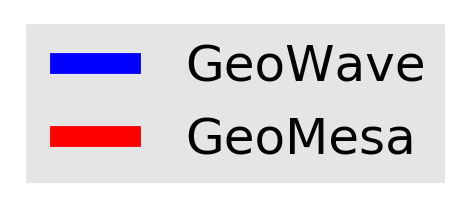
\includegraphics[width=0.20\textwidth]{../docs/img/legend.png}
%%   \caption{Legend.}
%%   \label{legend}
%% \end{wrapfigure}

\begin{figure}[h!tb]
  \centering
  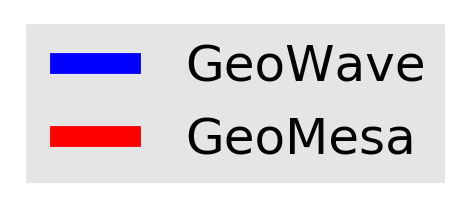
\includegraphics[width=0.20\textwidth]{../docs/img/legend.png}
  \caption{Legend.}
  \label{legend}
\end{figure}

\subsection{ GeoLife}

Test for GeoLife were performed on EMR 5.0.0 clusters of one m3.2xlarge master and three m3.2xlarge workers.
The GeoLife dataset was ingested with default 2D and 3D indexes for both systems.
See the appendix for details about machine specs and ingest results.

\subsubsection{Spatial queries of Beijing}

We used the Beijing geojson from Mapzen's borders dataset, which can be found in the resources of the \texttt{core} subproject.
This represents the multipolygon seen in Figure \ref{beijingpolygon}.

\begin{figure}[h!tb]
  \centering
  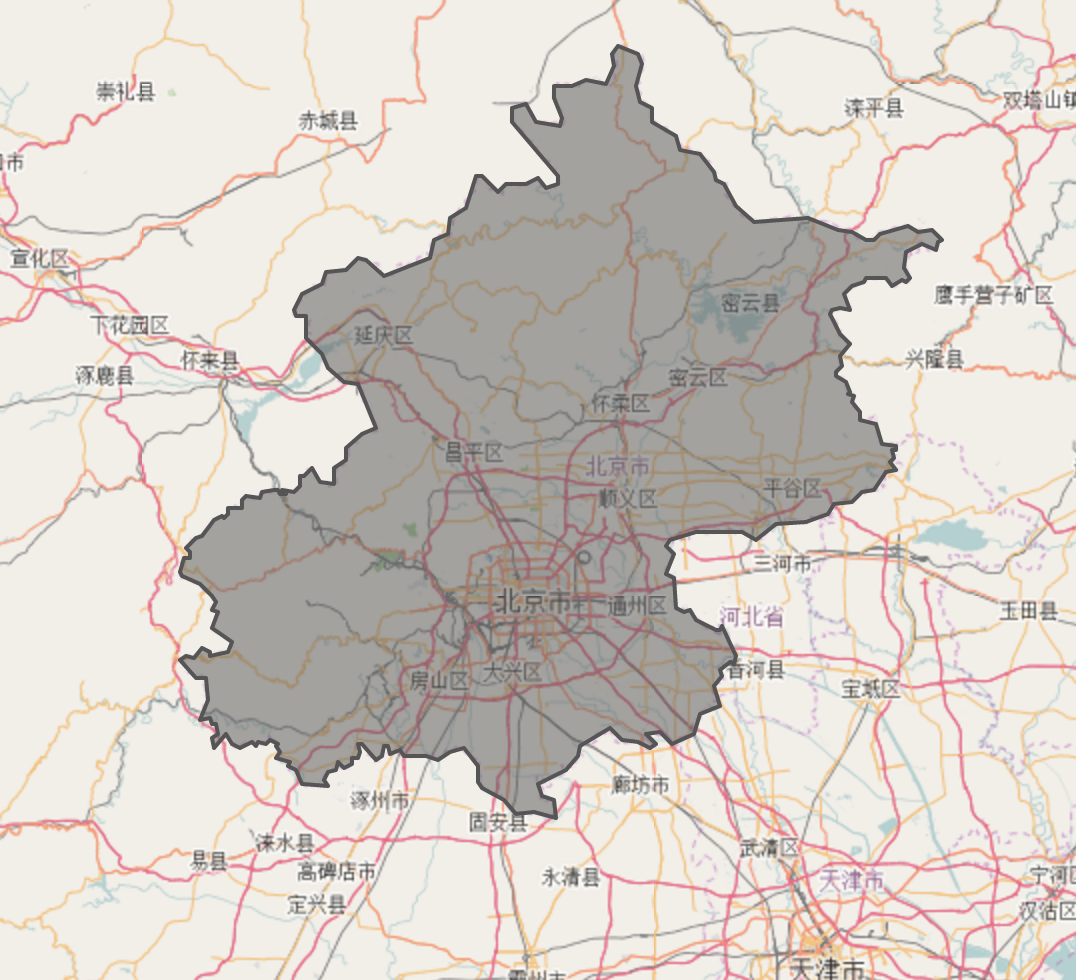
\includegraphics[width=0.60\textwidth]{../docs/img/beijing-poly.png}
  \caption{Beijing polygon.}
  \label{beijingpolygon}
\end{figure}

We then queried the city of Beijing over the whole time of the dataset.
We tracked results for both iterating over the resulting \texttt{SimpleFeature}s.
The timing results for that test, with outliers removed are shown in Figure \ref{beijingiterate}.

\begin{figure}[h!tb]
  \centering
  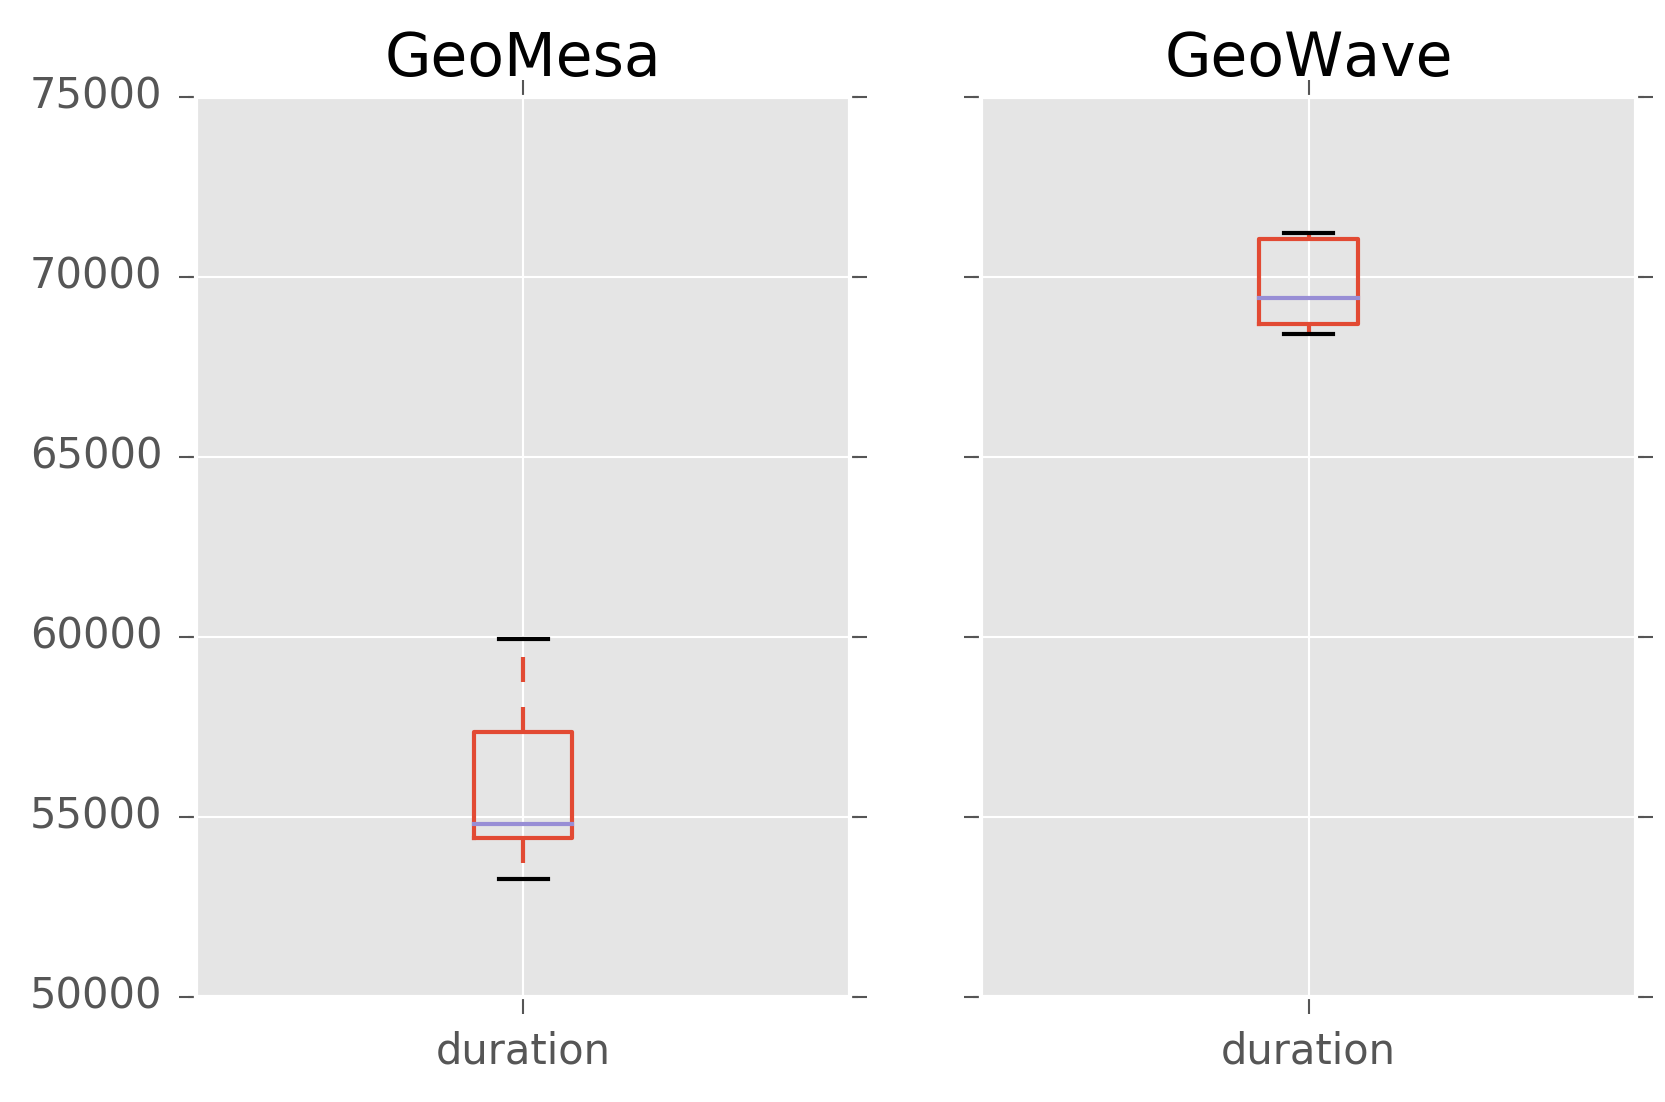
\includegraphics[width=0.60\textwidth]{../docs/img/geolife-beijing-iterate.png}
  %% \caption{Beijing polygon.}
  \label{beijingiterate}
\end{figure}

These queries take a long time; this makes sense, as they are iterating over $19,902,865$ results.

\subsubsection{Spatial queries of central Beijing}

To test on queries with smaller result set, we using \texttt{geojson.io} to draw a rough polygon around the center of Beijing.
We then performed spatial-only queries using the polygon shown in Figure \ref{beijingcenter}.

\begin{figure}[h!tb]
  \centering
  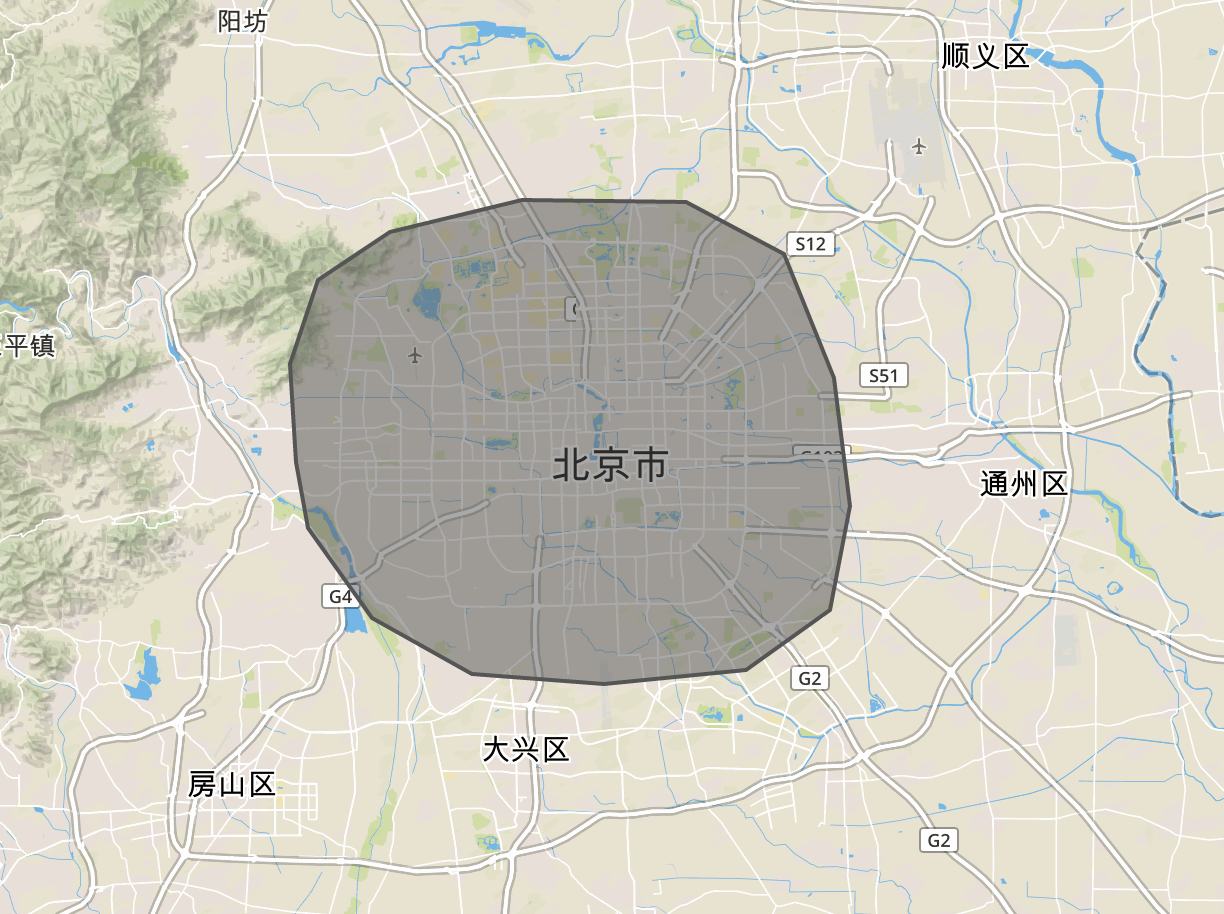
\includegraphics[width=0.60\textwidth]{../docs/img/beijing-center.png}
  \caption{Beijing center.}
  \label{beijingcenter}
\end{figure}

This allowed us to track the iteration and count queries against a smaller spatial extent.
However, this query did not actually cut out too many results; the result set for this query included $16,624,351$ results.
In Figure \ref{beijingcenteriterate}, outliers have been removed.

\begin{figure}[h!tb]
  \centering
  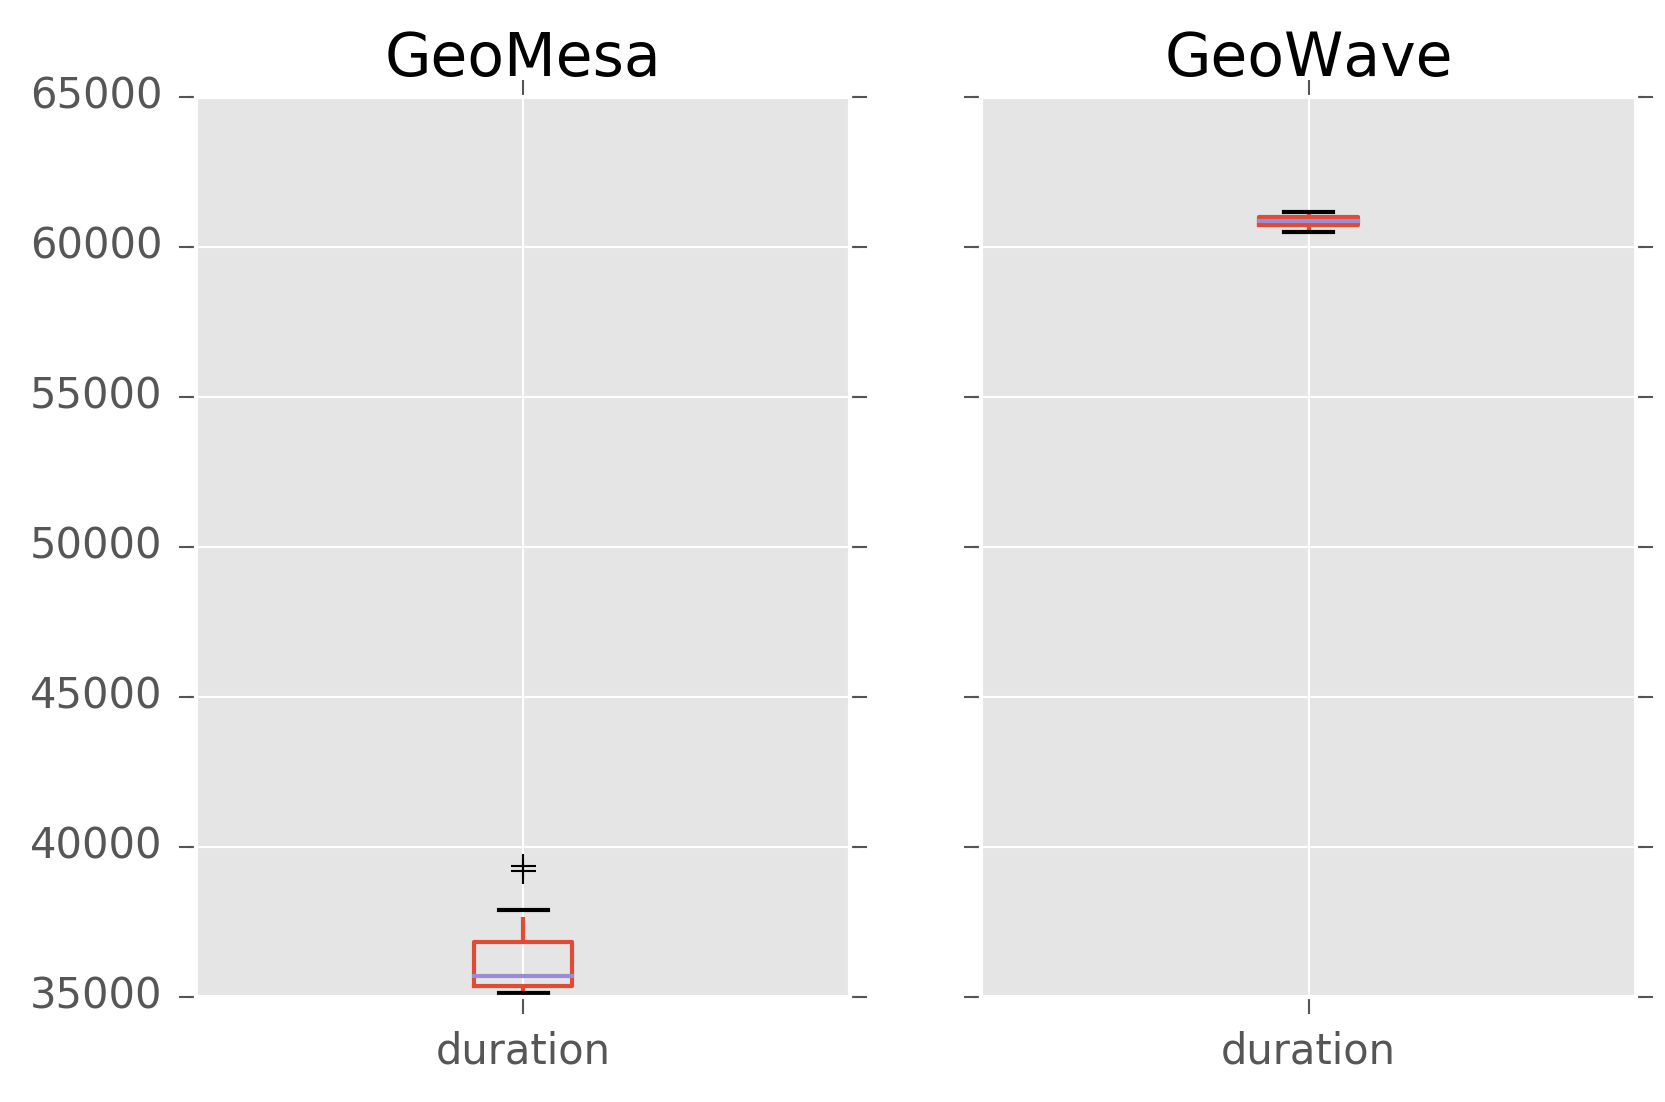
\includegraphics[width=0.60\textwidth]{../docs/img/geolife-beijing-center-iterate.png}
  \caption{Beijing center iterations.}
  \label{beijingcenteriterate}
\end{figure}

These two results show GeoMesa handling queries with large results faster than GeoWave, which is a result we've seen fairly consistently in our tests.

\subsubsection{Spatial queries of bounding boxes across Beijing}

This query cuts the bounding box of Beijing into \texttt{N} equal sized bounding boxes,
represented by the tile coordinate \texttt{COL} and \texttt{ROW}.

For instance, running \texttt{N=32} would create bounding boxes that look like those shown in Figure \ref{beijingbbox32}.

\begin{figure}[h!tb]
  \centering
  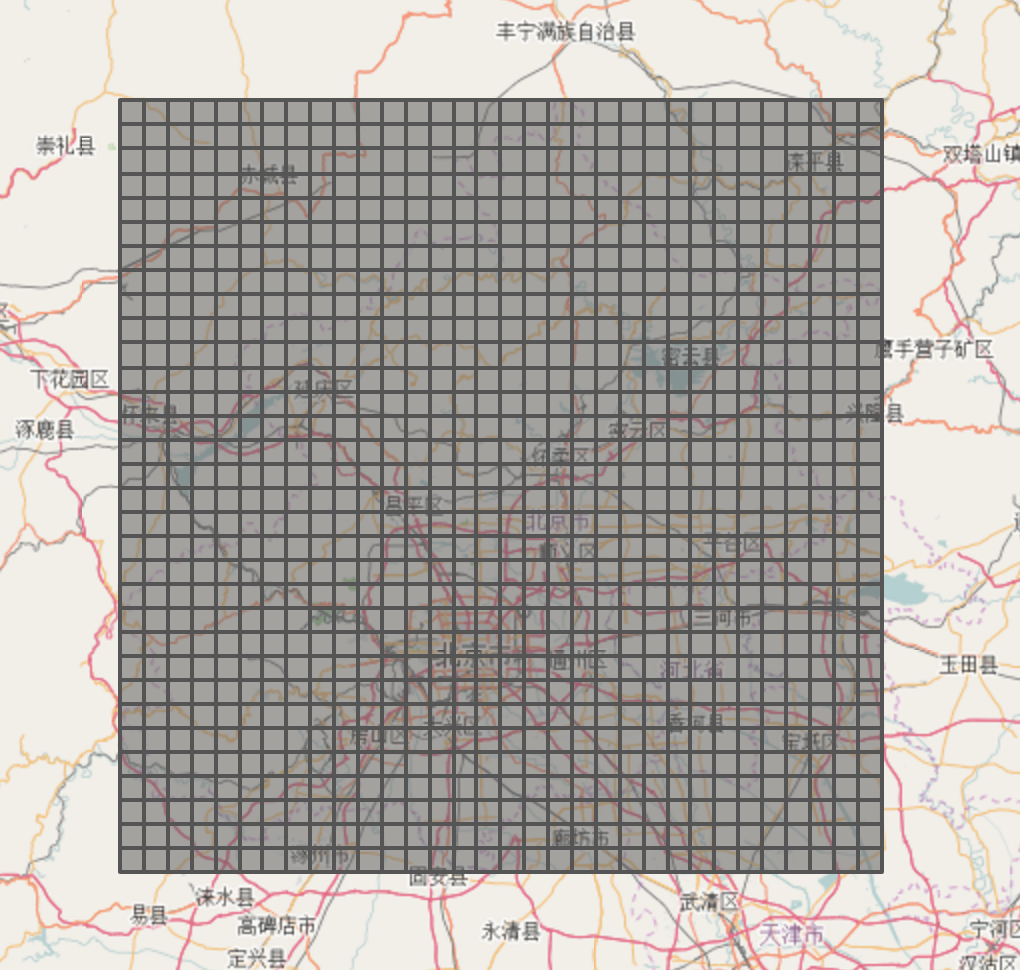
\includegraphics[width=0.60\textwidth]{../docs/img/beijing-bbox-32.png}
  \caption{Beijing bounding box for \texttt{N=32}.}
  \label{beijingbbox32}
\end{figure}

We tested with \texttt{N=32} \texttt{\{ 2, 4, 8, 16, 32\}}. This produced $1,024$ unique queries.
$417$ were queries with $0$ results, and were not considered.
$103$ of these queries did not produce the same result between GeoMesa and GeoWave;
a query for the entire bounding box of Beijing produces the same results,
so it is unclear why this mismatch occurs, and which system is incorrect.
Because these tests are focused on performance and not accuracy, these mismatched results are included in the graphs below.

The graph in Figure \ref{beijingscatter} plots the result count of each query against the duration of that query per system:

\begin{figure}[h!tb]
  \centering
  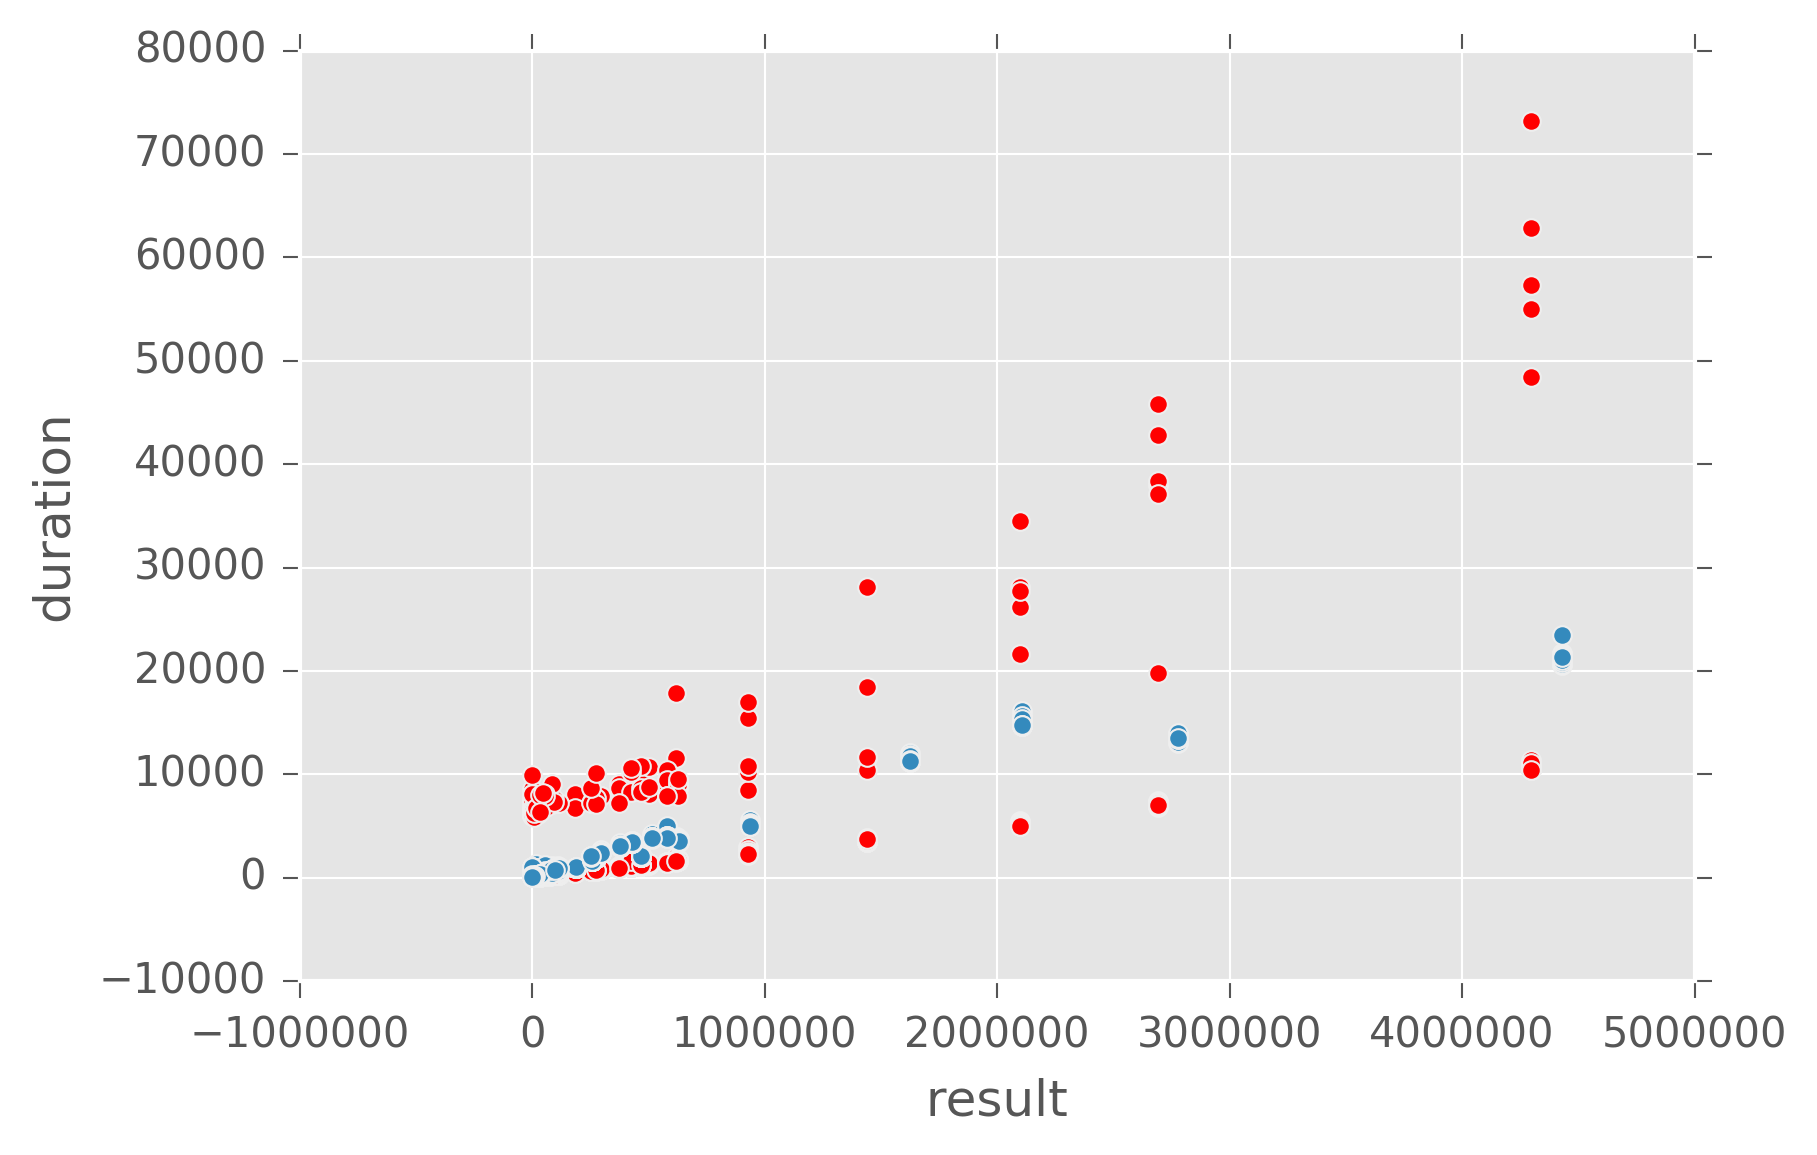
\includegraphics[width=0.60\textwidth]{../docs/img/geolife-bbox-scatter.png}
  \caption{Beijing iteration scatter plot.}
  \label{beijingscatter}
\end{figure}

This shows GeoMesa having more variance over duration; however it does not give a good indication of trends.
If we plot a linear regression on the two set of points, we can see that although GeoMesa appears to have
more variance in query duration, the queries typically return faster from GeoMesa than from GeoWave, and this
trend becomes more pronounced as the number of results increases (please see Figure \ref{beijingscatterreg}).

\begin{figure}[h!tb]
  \centering
  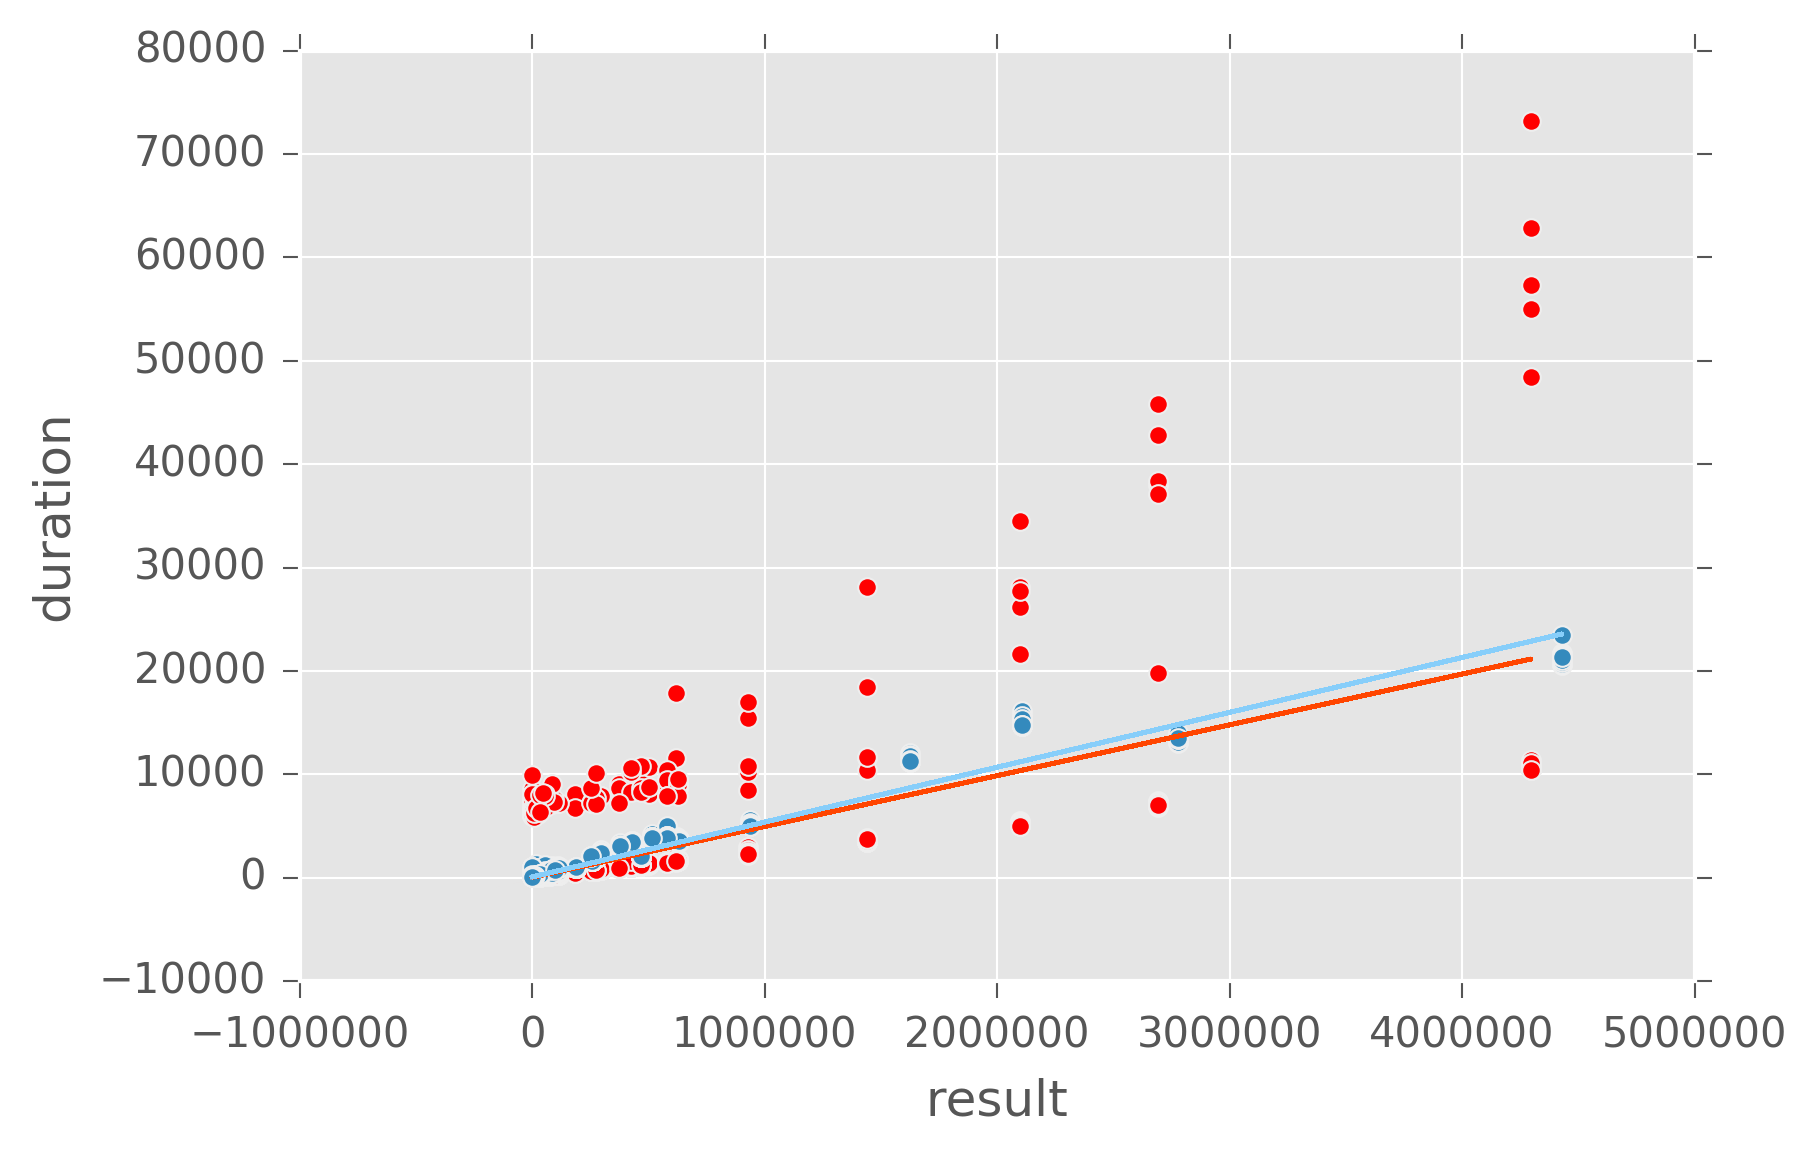
\includegraphics[width=0.60\textwidth]{../docs/img/geolife-bbox-scatter-with-regression.png}
  \caption{Beijing iteration scatter plot with regression.}
  \label{beijingscatterreg}
\end{figure}

GeoMesa has a feature called ``loose bbox'' that allows you to trade performance for result accuracy;
it only uses the space filling curve to filter data and does no secondary filtering, so false positives
could be returned. The graph below includes a scatterplot and regression for the loose bounding box queries in yellow
(please see Figure \ref{beijingloosescatterreg}).

\begin{figure}[h!tb]
  \centering
  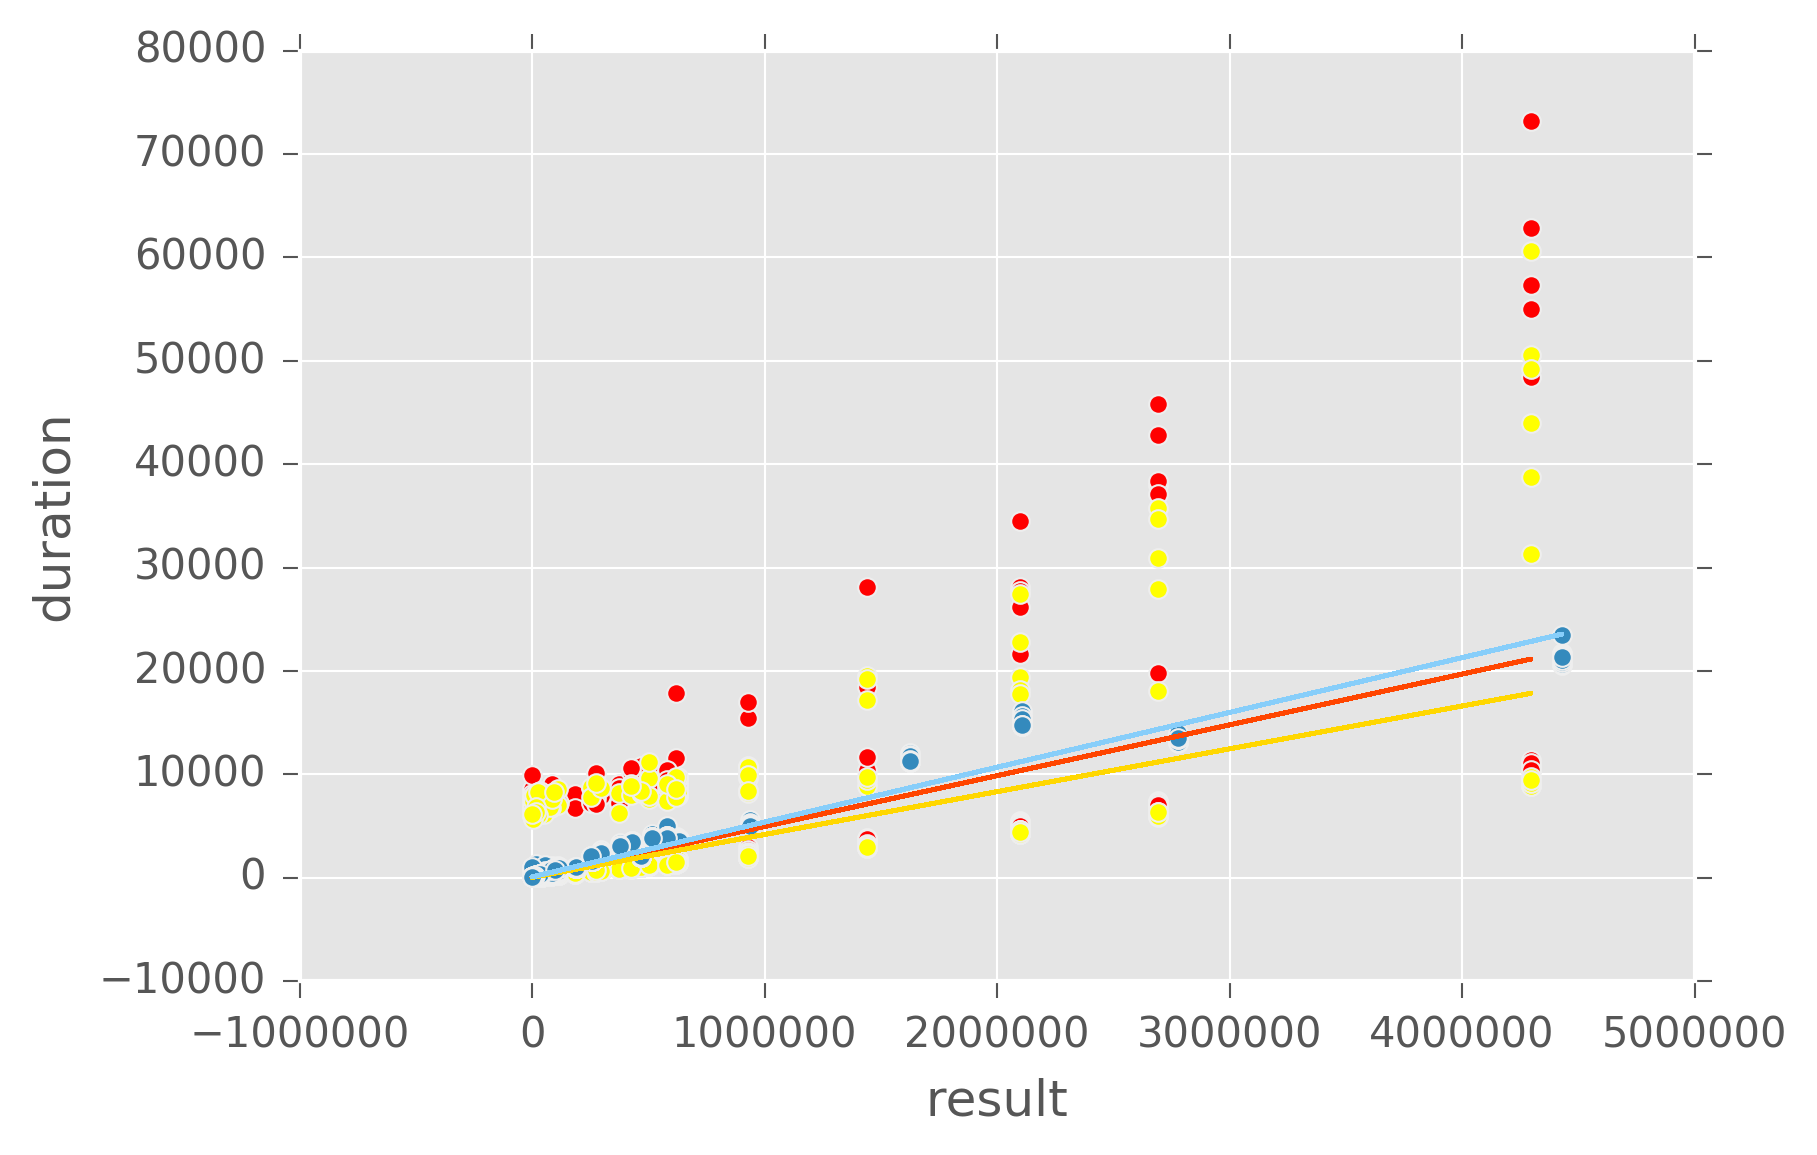
\includegraphics[width=0.60\textwidth]{../docs/img/geolife-bbox-regression-with-loose.png}
  \caption{Beijing ``loose bbox'' scatter plot with regression.}
  \label{beijingloosescatterreg}
\end{figure}

The graph in Figure \ref{beijingloosescatterreg2} shows the regressions against queries returning less than $10,000$ results.
It shows that even for queries with lower result counts, GeoMesa tends to slightly outperform GeoWave
for these spatial-only point data queries, for both loose and exact queries.

\begin{figure}[h!tb]
  \centering
  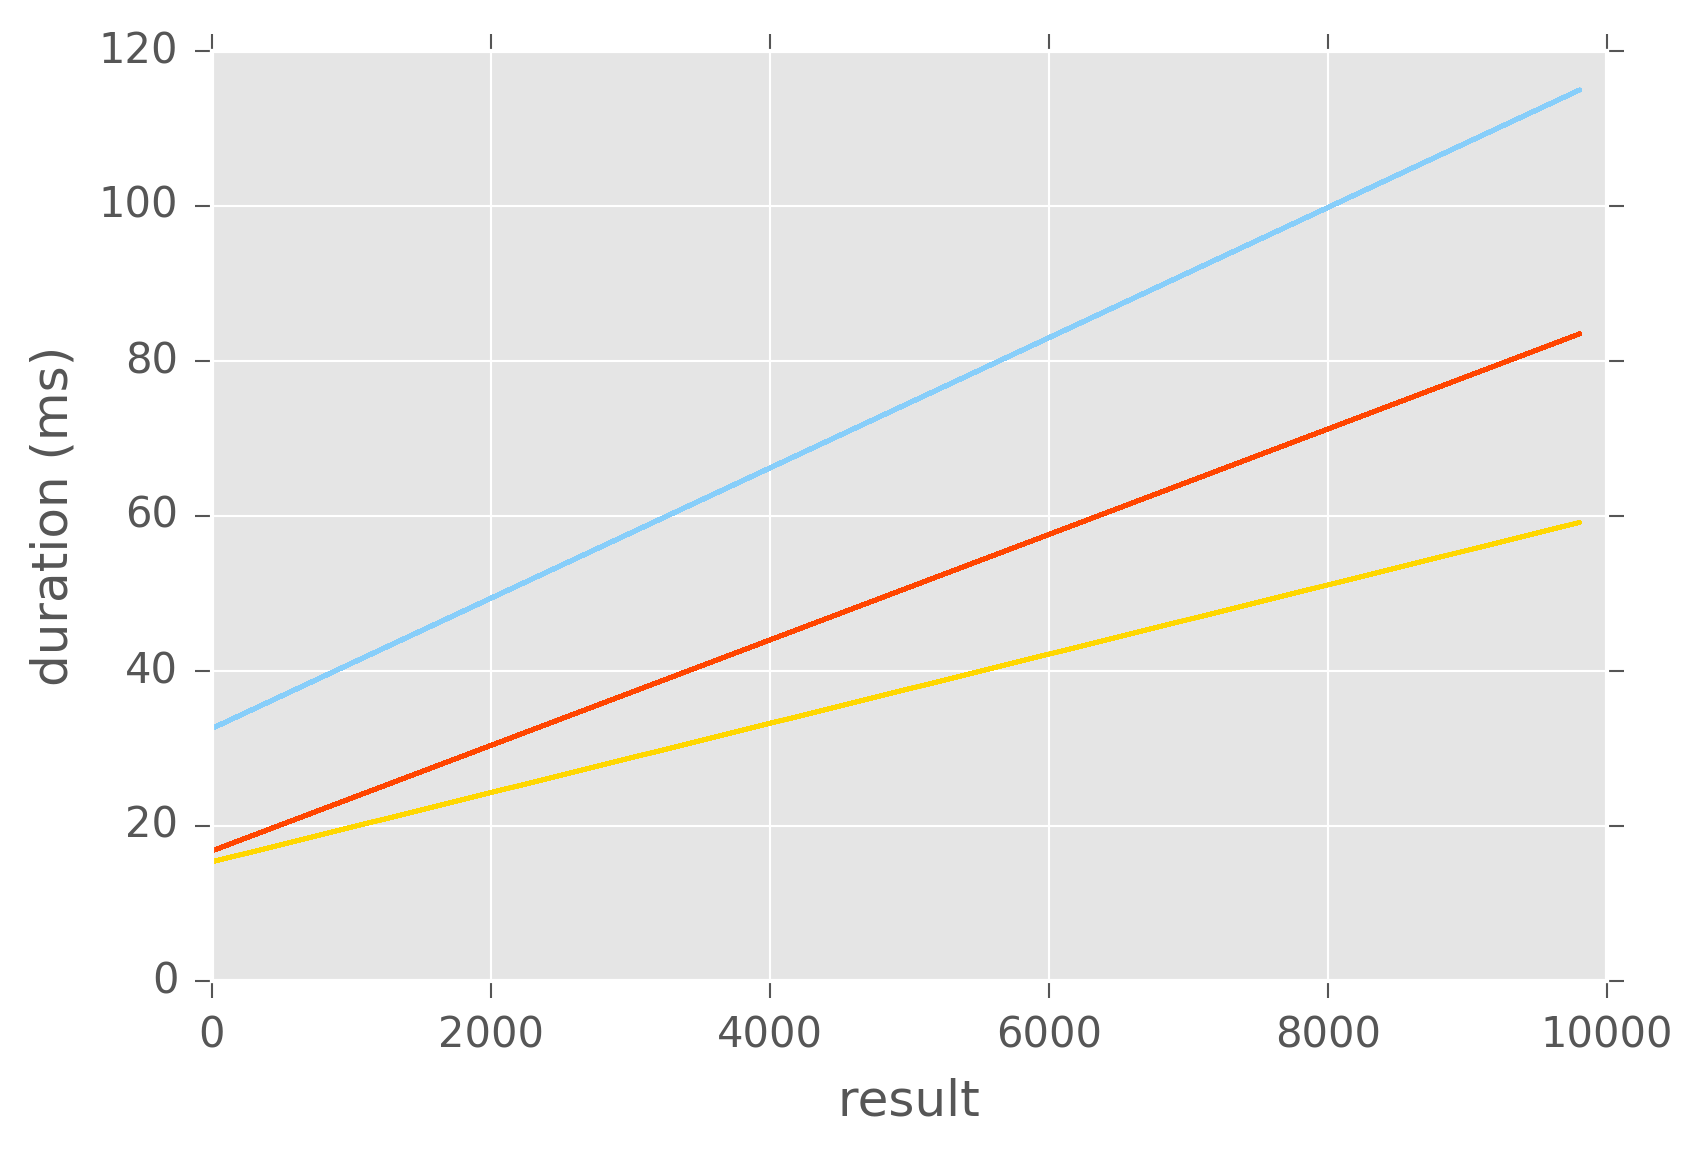
\includegraphics[width=0.60\textwidth]{../docs/img/geolife-bbox-regression-with-loose-less-than-10000.png}
  \caption{Beijing ``loose bbox'' scatter plot with regression, fewer than $10,000$ results.}
  \label{beijingloosescatterreg2}
\end{figure}

\subsubsection{Spatiotemporal query results}

In both systems, spatiotemporal queries (those with bounds in both space and time) hit a different table and indexing mechanism than the spatial-only queries described above.
To include a temporal aspect to our queries, we ran a query over the center of Beijing for the month of August in 2011.
This returned $84,496$ results.
In Figure \ref{beijingjan2011}, outliers have been removed.

\begin{figure}[h!tb]
  \centering
  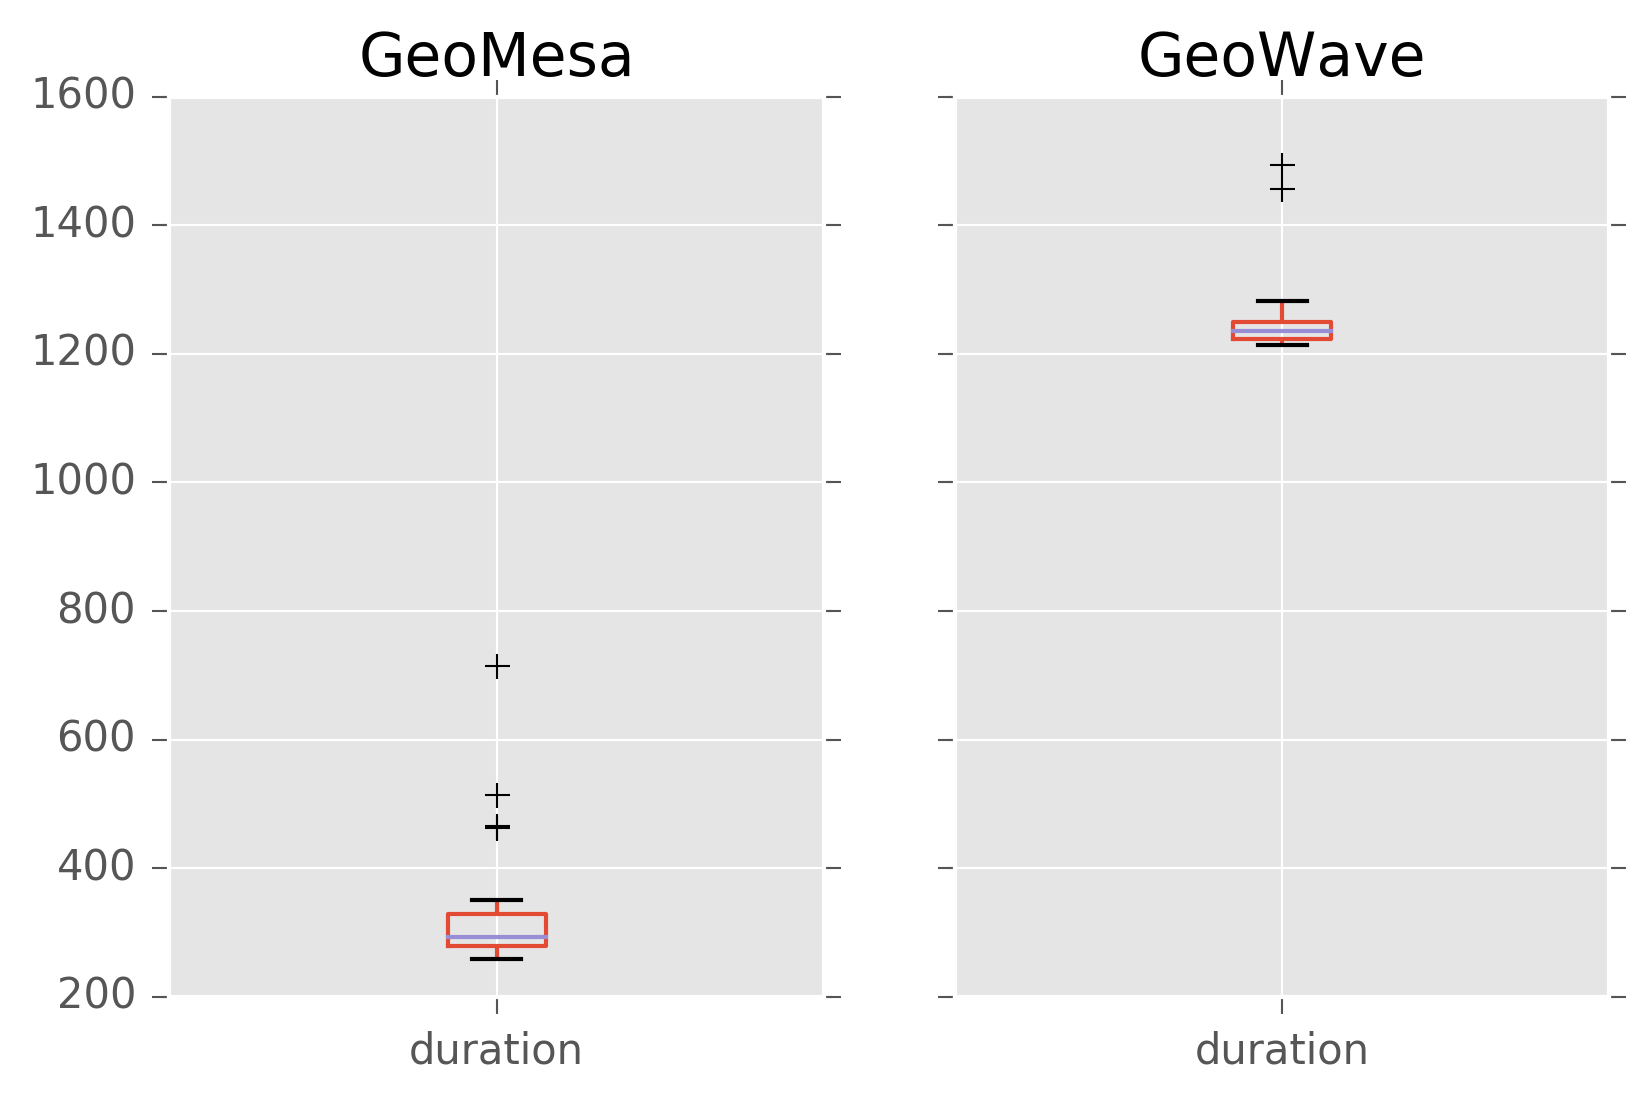
\includegraphics[width=0.60\textwidth]{../docs/img/geolife-beijing-center-aug-2011.png}
  \caption{Beijing January 2011 iterations.}
  \label{beijingjan2011}
\end{figure}

We see that GeoMesa performs better in this query.
If we plot the histogram of GeoMesa durations with outliers removed,
for both exact and loose (red and yellow, respectively), and compare it to the histogram of durations for GeoWave queries with outliers removed,
we see that there is a wider spread of timing results coming from GeoWave for this query.

\begin{figure}[h!tb]
  \centering
  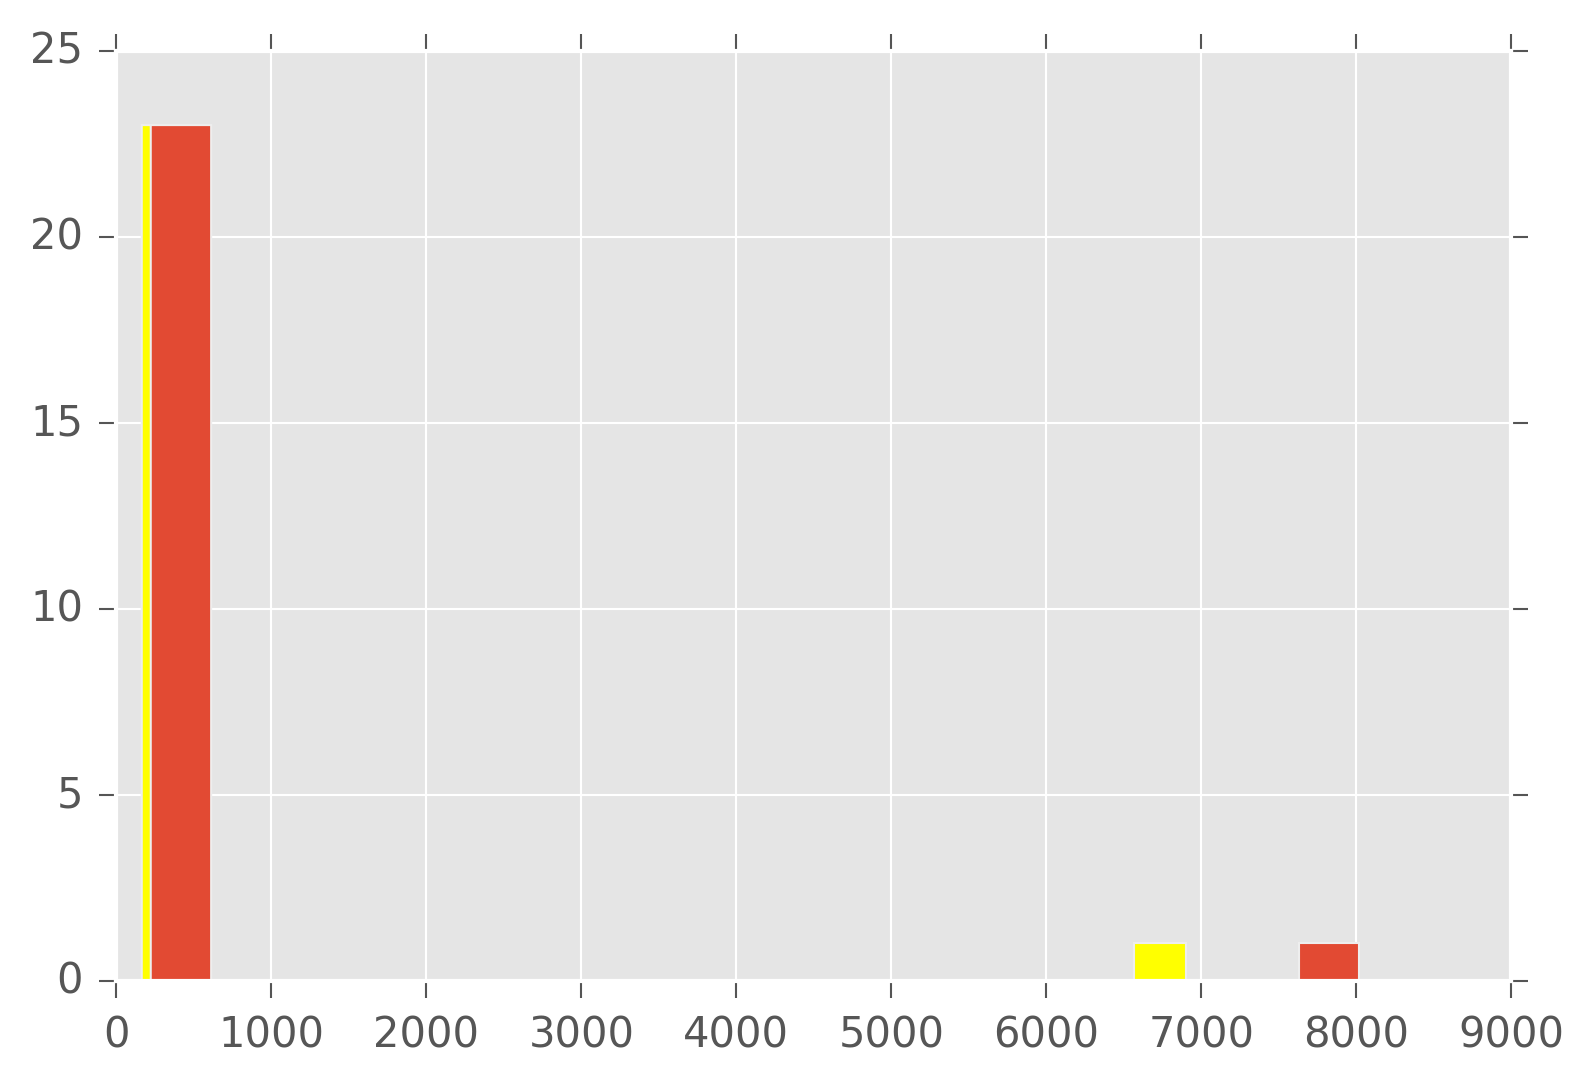
\includegraphics[width=0.45\textwidth]{../docs/img/geolife-beijing-center-feb-2011-bbox-gm.png}
  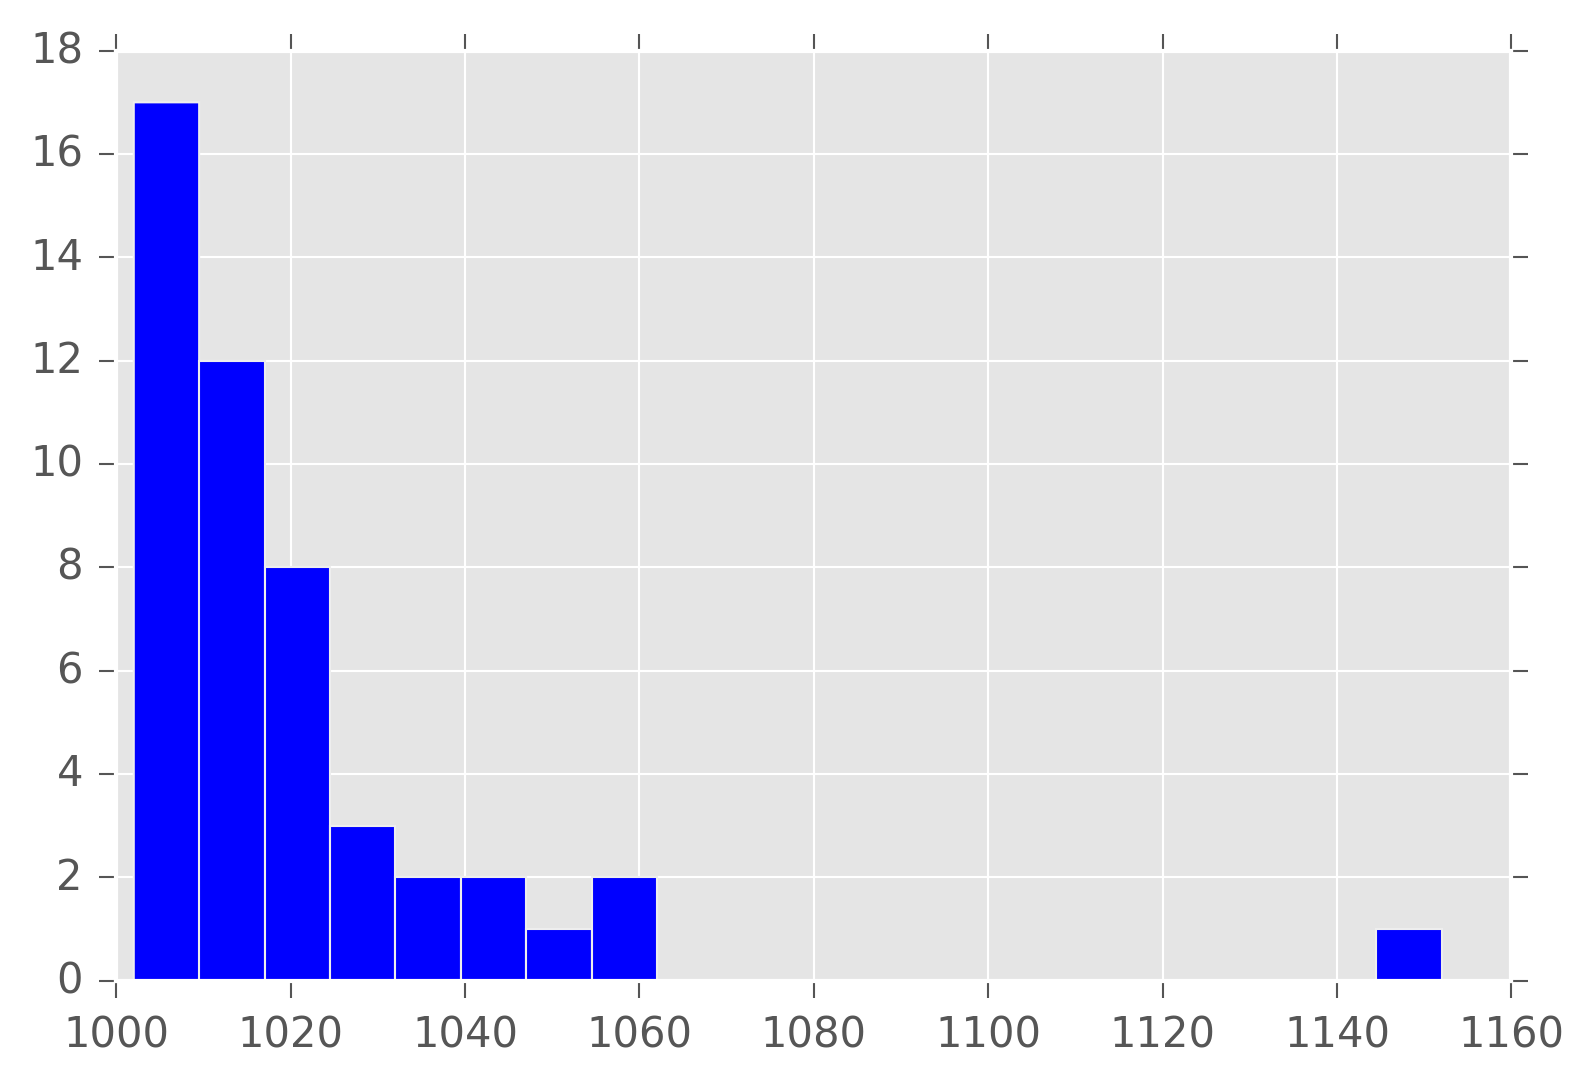
\includegraphics[width=0.45\textwidth]{../docs/img/geolife-beijing-center-feb-2011-bbox-gw.png}
  \caption{Beijing February 2011 iterations.}
  \label{beijingfebg2011}
\end{figure}


\subsection{GDELT}

Test for GDELT were performed on EMR 5.0.0 clusters of one \texttt{m3.2xlarge} master and five \texttt{m3.2xlarge} workers.

\subsubsection{Spatiotemporal queries of areas around cities: City Buffers}

For these queries, which we call the ``city buffer'' tests, queries are taken from center points corresponding to the following cities:
Paris, Philadelphia, Istanbul, Baghdad, Tehran, Beijing, Tokyo, Oslo, Khartoum, and Johannesburg.
For instance, the Paris city buffers can be seen in Figure \ref{paris}.

\begin{figure}[h!tb]
  \centering
  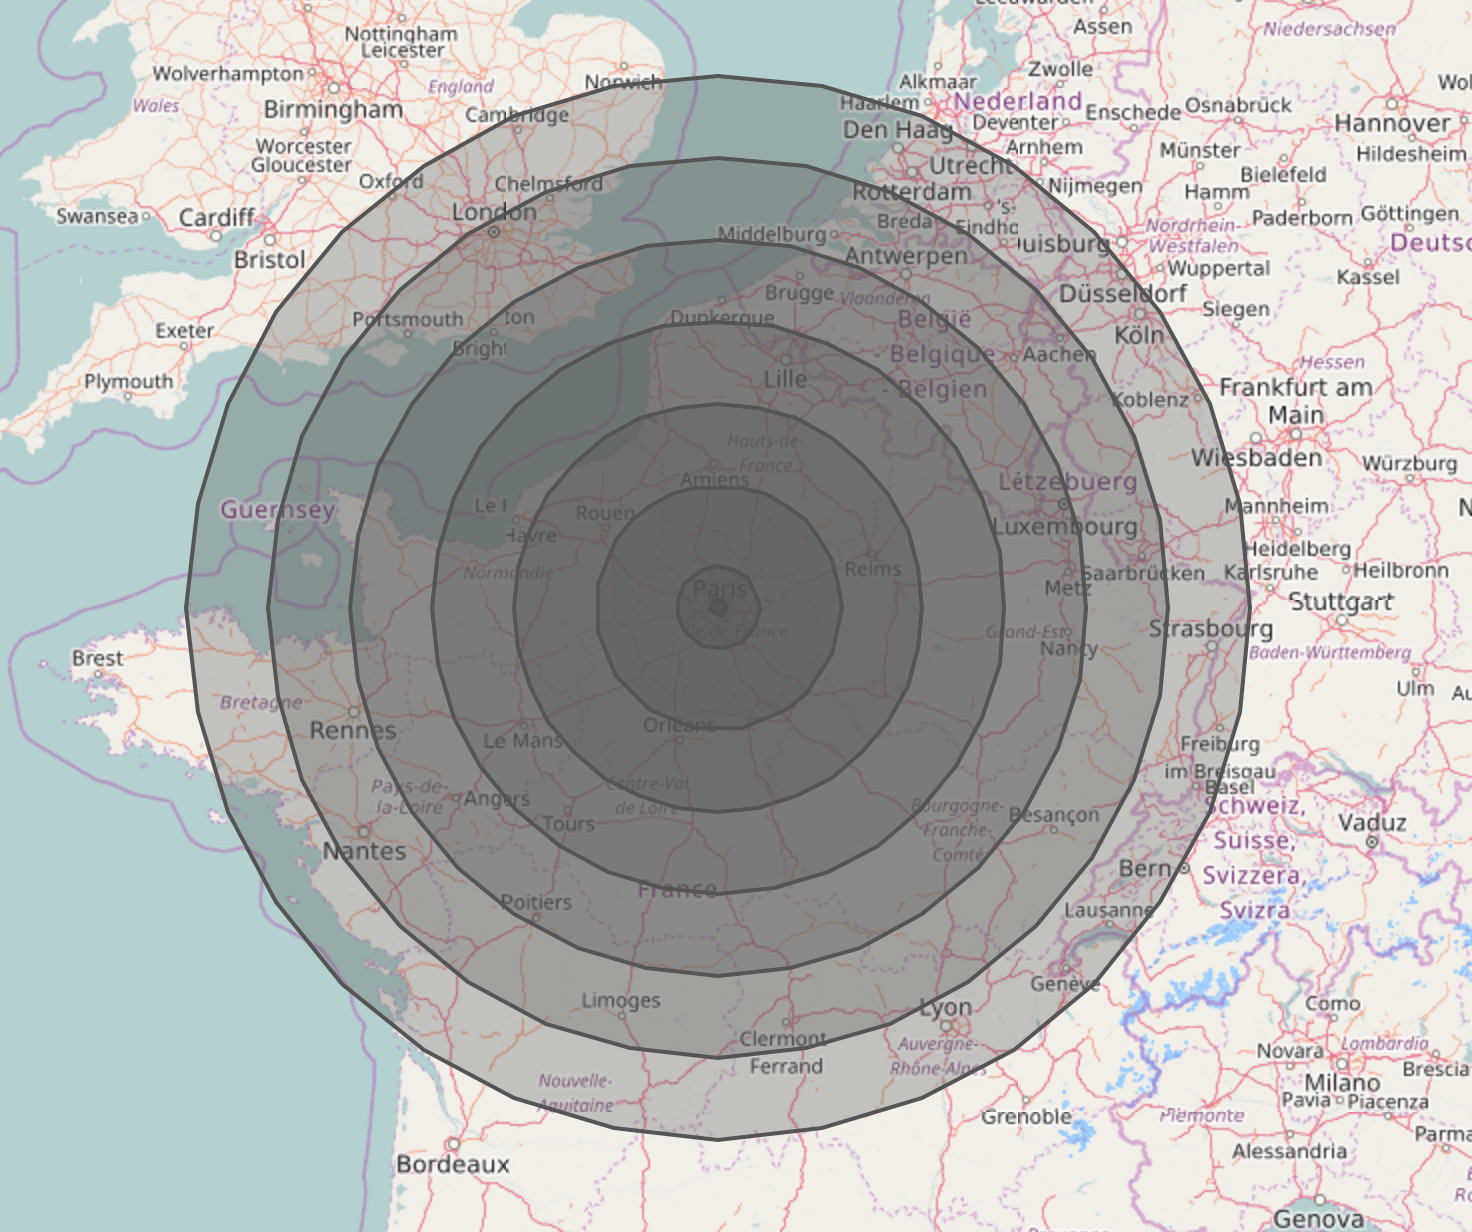
\includegraphics[width=0.60\textwidth]{../docs/img/gdelt/paris-city-buffers.png}
  \caption{Paris city buffers.}
  \label{paris}
\end{figure}

The queries were taken over a set of these durations: six months, two months, two weeks, and six days.

Figure \ref{durationbyresult} contains a scatter plot of duration by query result count.

\begin{figure}[h!tb]
  \centering
  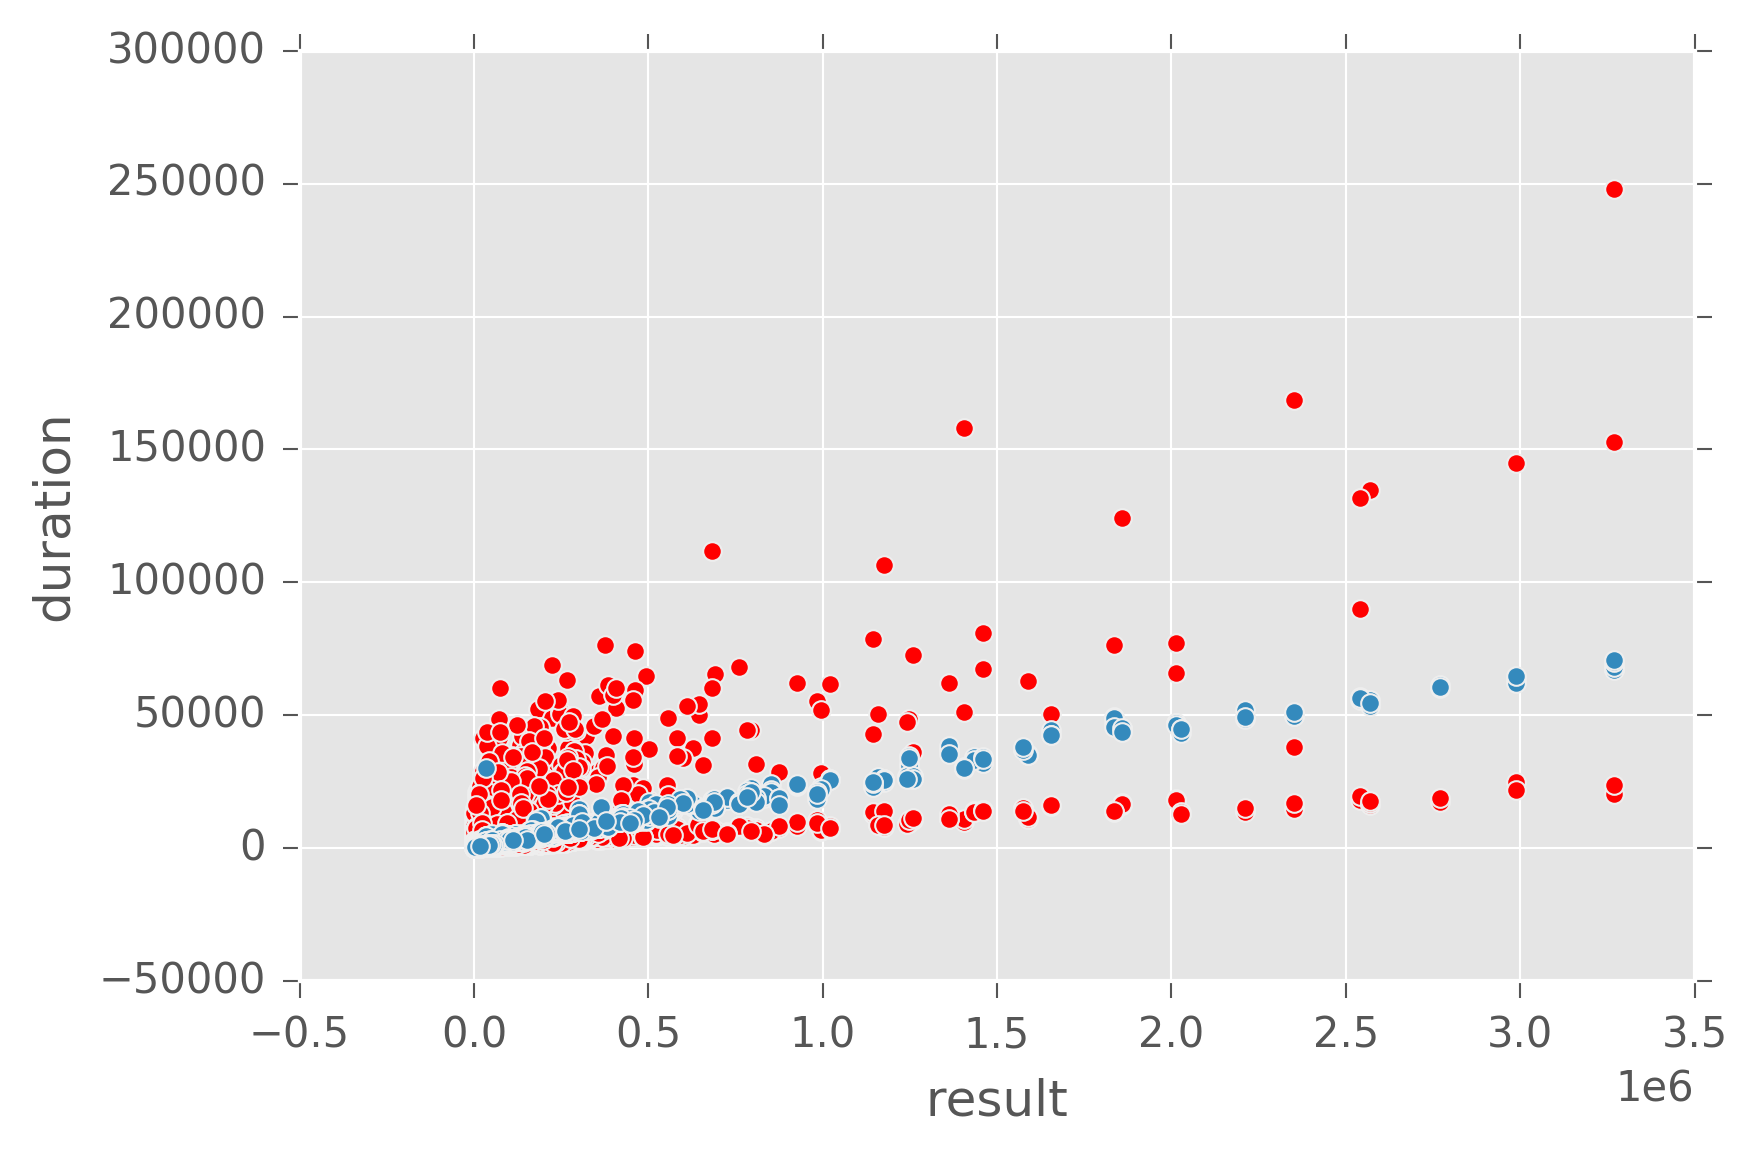
\includegraphics[width=0.60\textwidth]{../docs/img/gdelt/gdelt-result-over-duration.png}
  \caption{Duration by result count.}
  \label{durationbyresult}
\end{figure}

We can see that GeoMesa has much less consistent results than GeoWave.
If we plot a linear regression on this point sets, we'll get what is shown in Figure \ref{durationbyresultreg}.

\begin{figure}[h!tb]
  \centering
  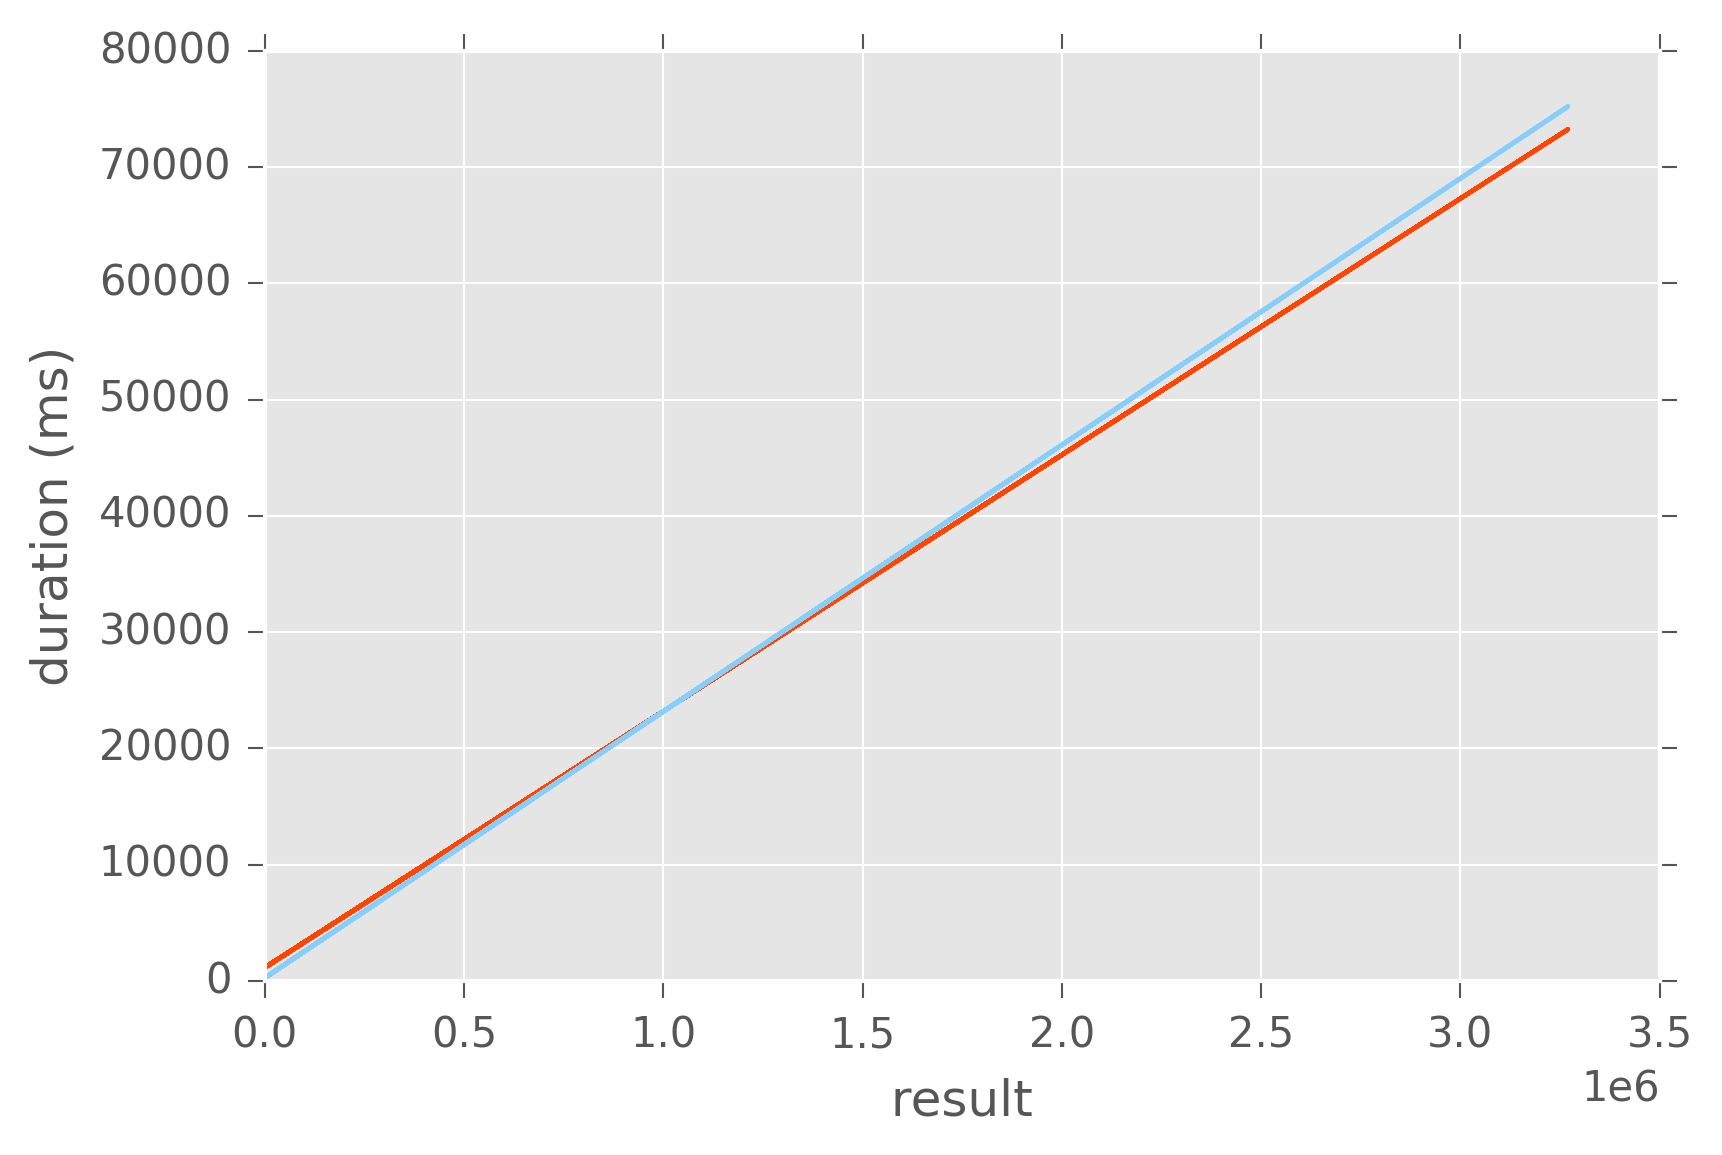
\includegraphics[width=0.60\textwidth]{../docs/img/gdelt/gdelt-result-over-duration-regression.png}
  \caption{Duration by result regression.}
  \label{durationbyresultreg}
\end{figure}

GeoMesa tends to be slower at returning these queries than GeoWave, until the queries return a large number of results.
According to the regression, after around 1 million results returned, GeoMesa becomes faster than GeoWave.
This is an imprecise result, but one that we have found consistent over point datasets: GeoMesa generally does better with queries that produce large result sets.

Figure \ref{durationresultall14} shows the mean duration of queries over all cities and all buffer sizes, for 14 day queries, based on the result count of the queries.
The $x$-axis in this case represents a bin of result counts;
points were averaged according to a quantile-based discretization function of result count,
which is represented here on the $x$-axis as the lowest result count of that grouping.

\begin{figure}[h!tb]
  \centering
  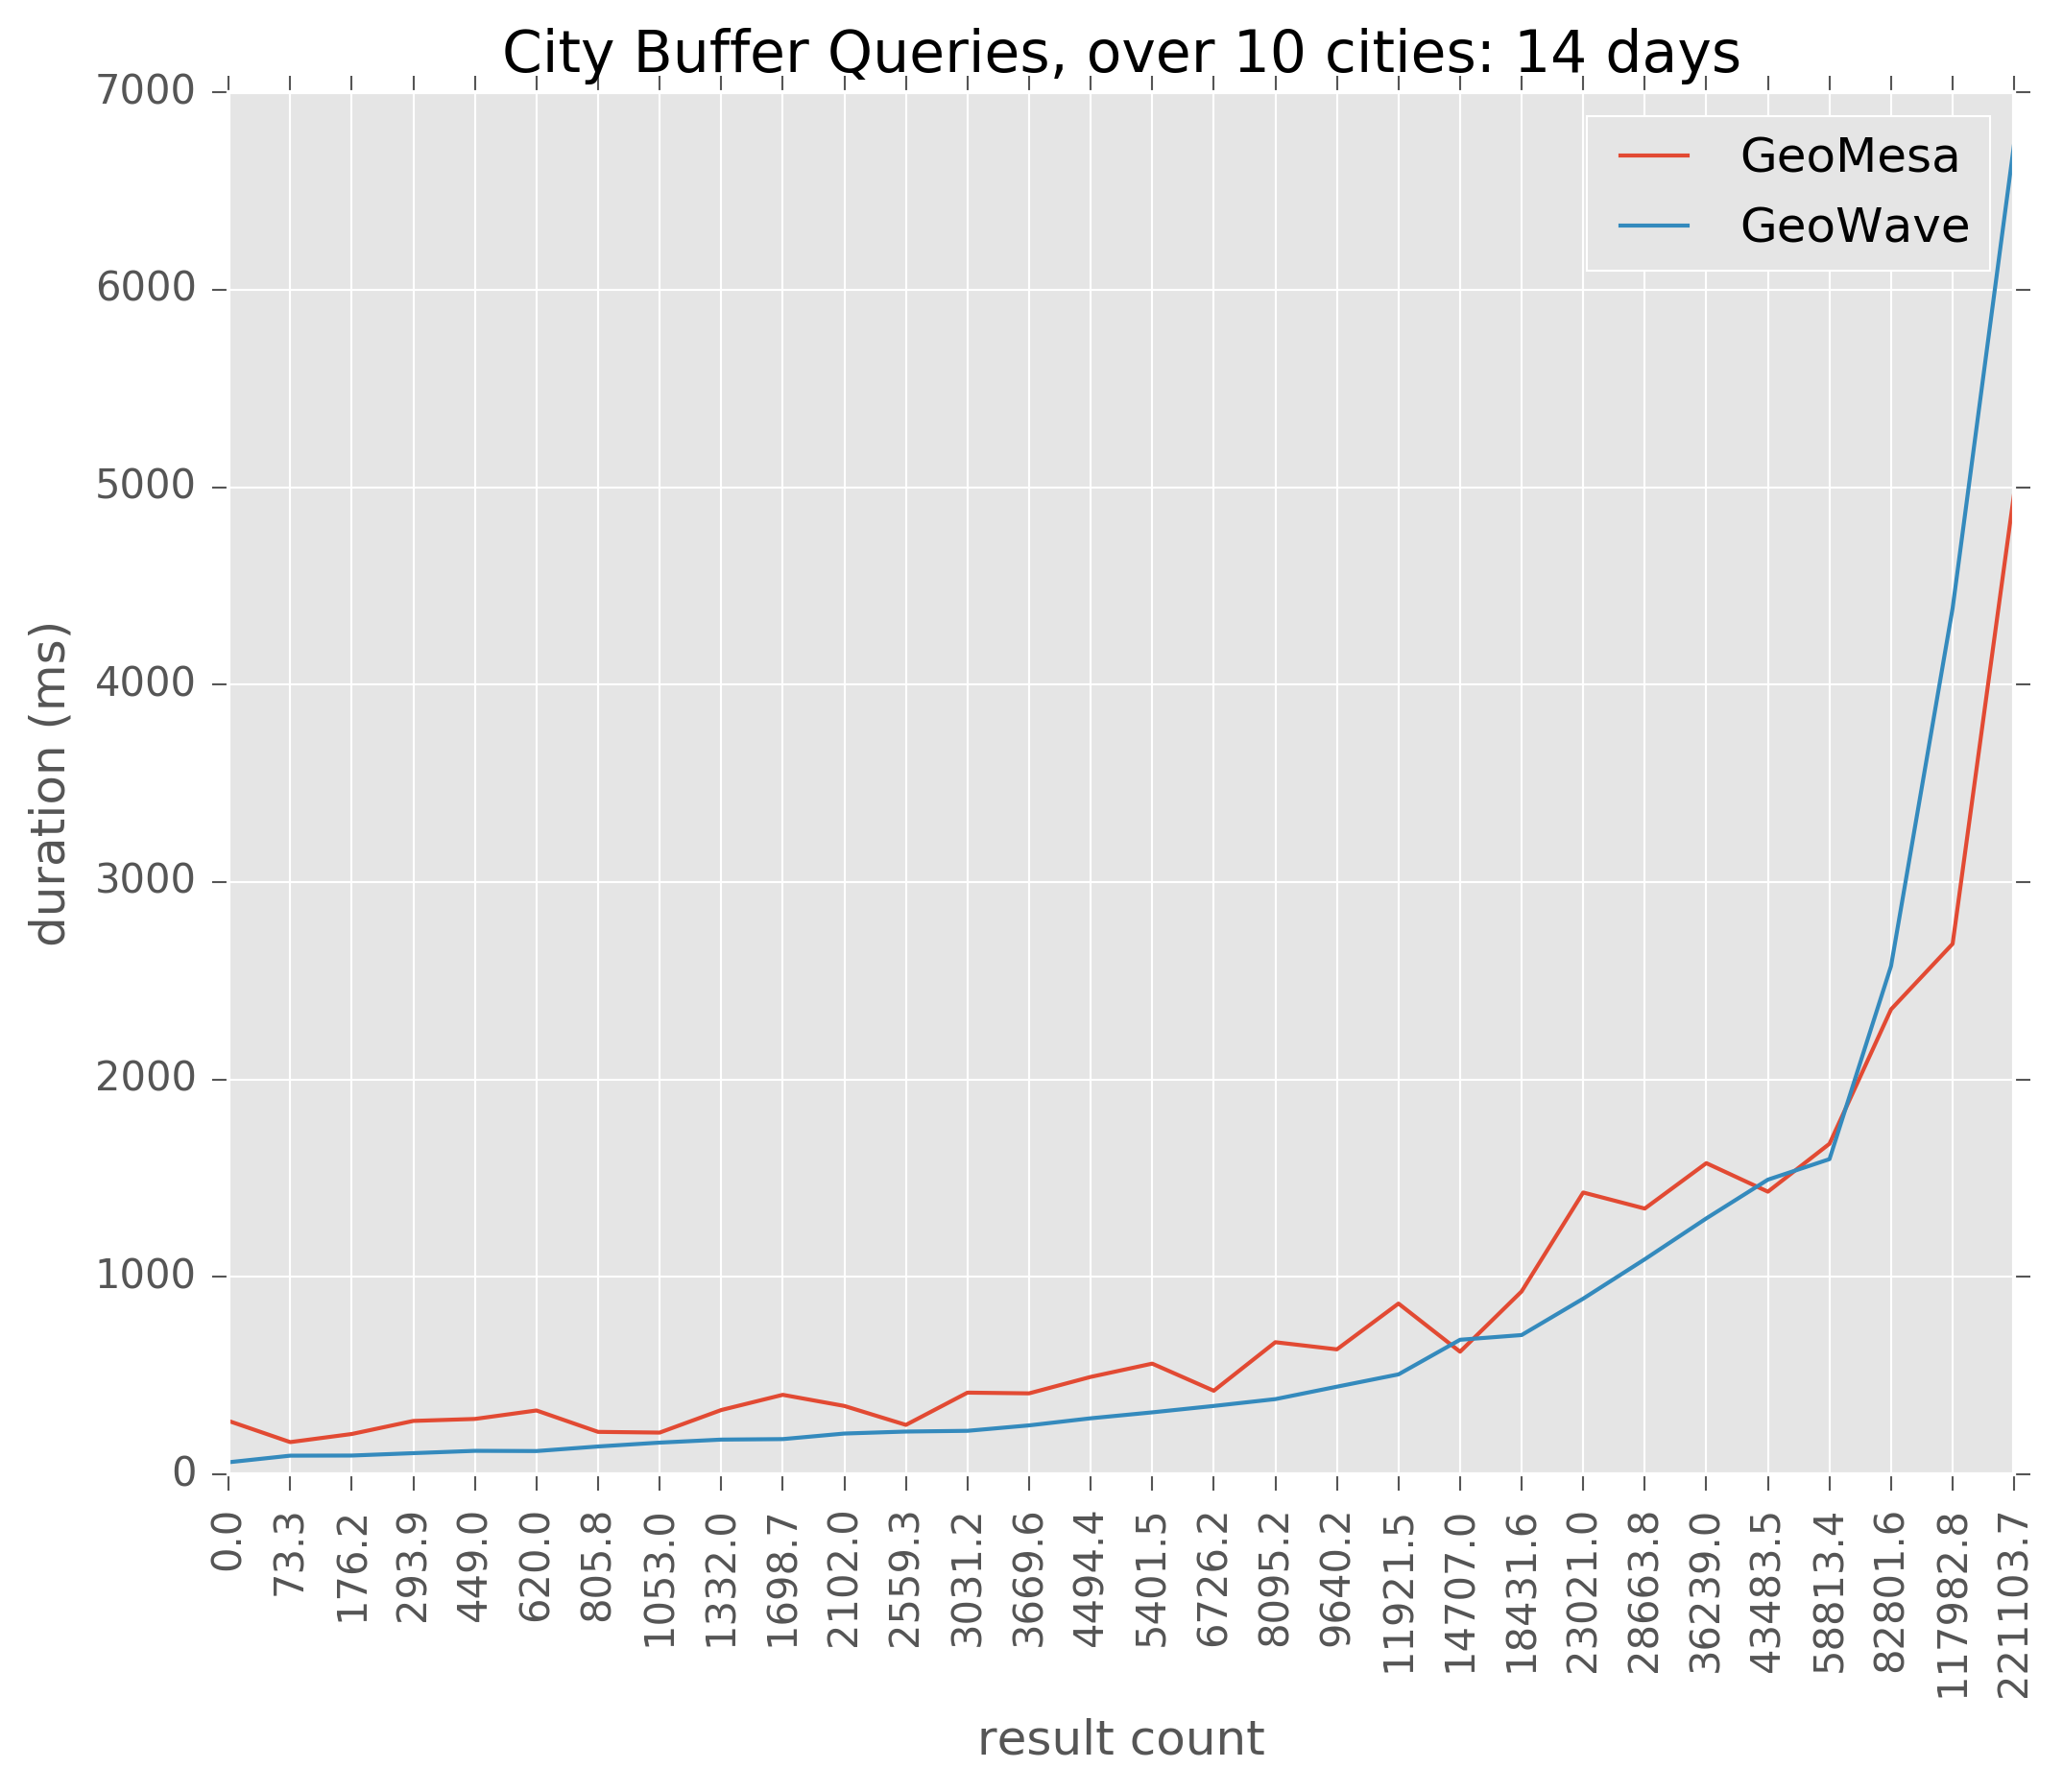
\includegraphics[width=0.60\textwidth]{../docs/img/gdelt/014-days-default.png}
  \caption{Durations over result counts, default indexes, all queries of 14 days.}
  \label{durationresultall14}
\end{figure}

We see here that again GeoMesa appears to be slower than GeoWave,
until a certain result count is reached,
after which it performs better.

If we take a look at the next graph, another pattern emerges.
Figure \ref{durationresultall168} moves the temporal bounds of the query to $168$ days.

\begin{figure}[h!tb]
  \centering
  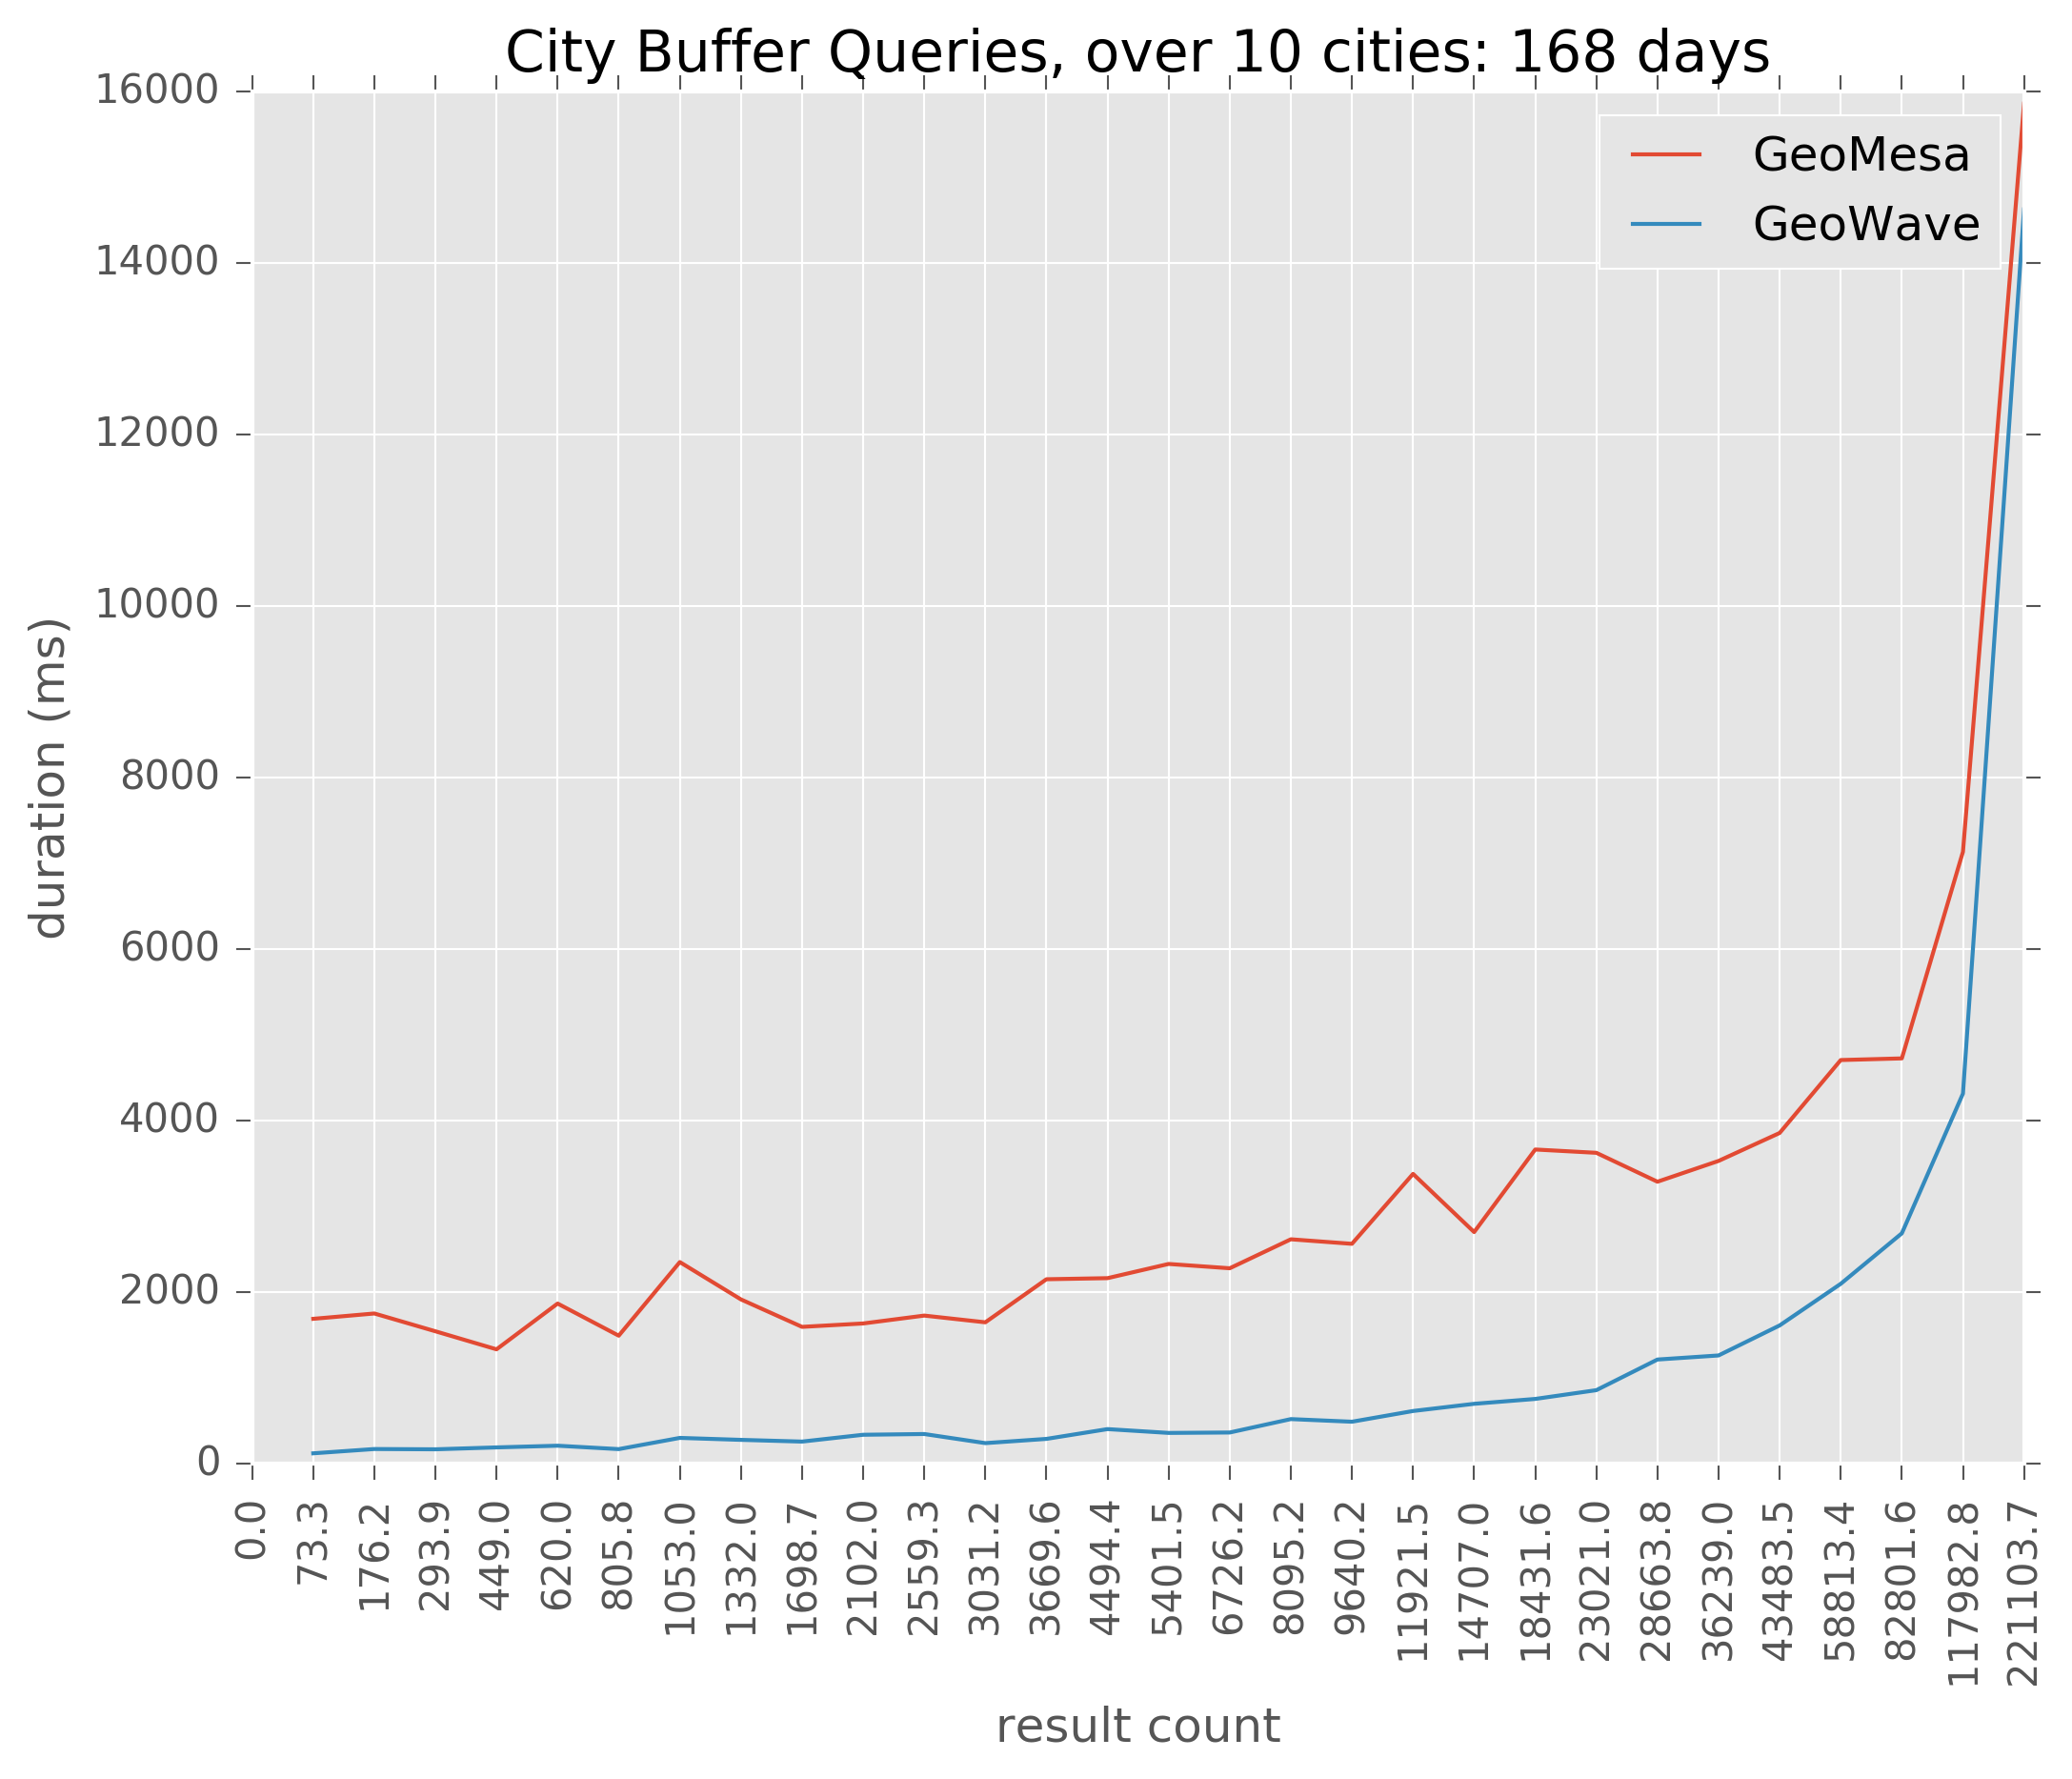
\includegraphics[width=0.60\textwidth]{../docs/img/gdelt/168-days-default.png}
  \caption{Durations over result counts, default indexes, all queries of $168$ days.}
  \label{durationresultall168}
\end{figure}

We see GeoMesa performing worse than the $14$ day case.
In this case it actually never crosses the threshold where it starts outperforming GeoWave based on result count
(according to this technique of averaging result count).

\subsubsection{Index configurations}

We hypothesized that some of the timing differences we were seeing here was because of differences in the configuration
of their indexing mechanisms. As described in the section comparing the index configurations, the default periodicity
for GeoMesa is one week, while in GeoWave it is one year. Also, GeoWave does not shard it's data by default.
To find out how this configuration might be affecting the timing results, we tested with both systems set
to having the following configuration:

\begin{itemize}
\item Both systems configured to have a periodicity of one month, with default sharding
\item Both systems configured to have a periodicity of one year, with default sharding
\item Both systems configured to have a periodicity of one year, with 4 shards being generated by a hashing algorithm
\end{itemize}

We attempted to test a configuration where both systems had a periodicity of one week, but this configuration
produces GeoWave results that were incorrect.

The last configuration in the list above produced improvements in timing results for the City Buffer queries, which we will explore below,
and be referred to as the ``matched'' index configuration.

Figure \ref{matching14} shows the durations of $14$ day queries averages broken into the same result count quartiles.
We can see a marked improvement in GeoMesas results.

\begin{figure}[h!tb]
  \centering
  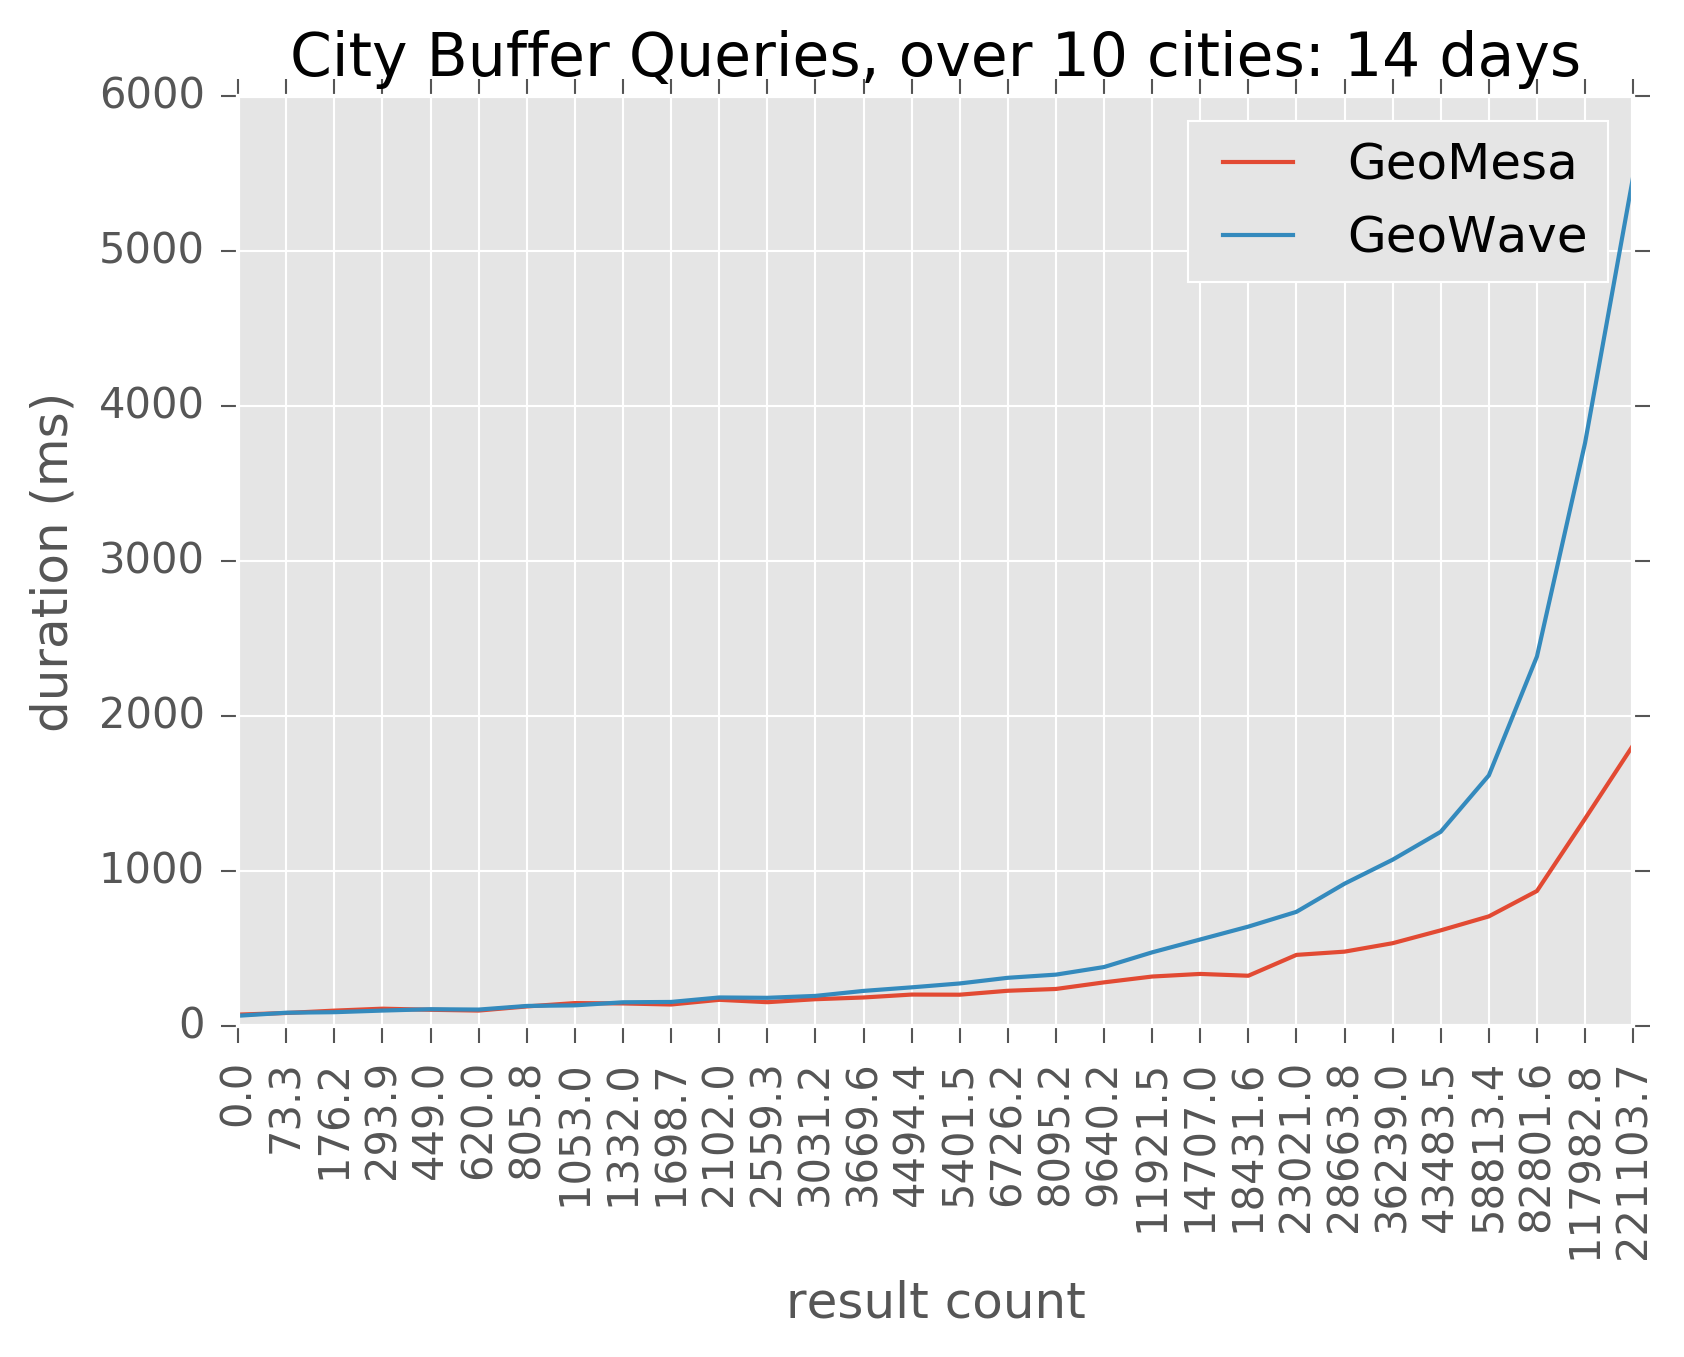
\includegraphics[width=0.60\textwidth]{../docs/img/gdelt/014-days-matching.png}
  \caption{Durations over result counts, matching indexes, all queries of $14$ days.}
  \label{matching14}
\end{figure}

In the case of the $168$ day queries, we see that although there is still a degradation of performance for GeoMesa,
it is not nearly as prominent as it was with the default indexing.
Please see Figure \ref{matching168}.

\begin{figure}[h!tb]
  \centering
  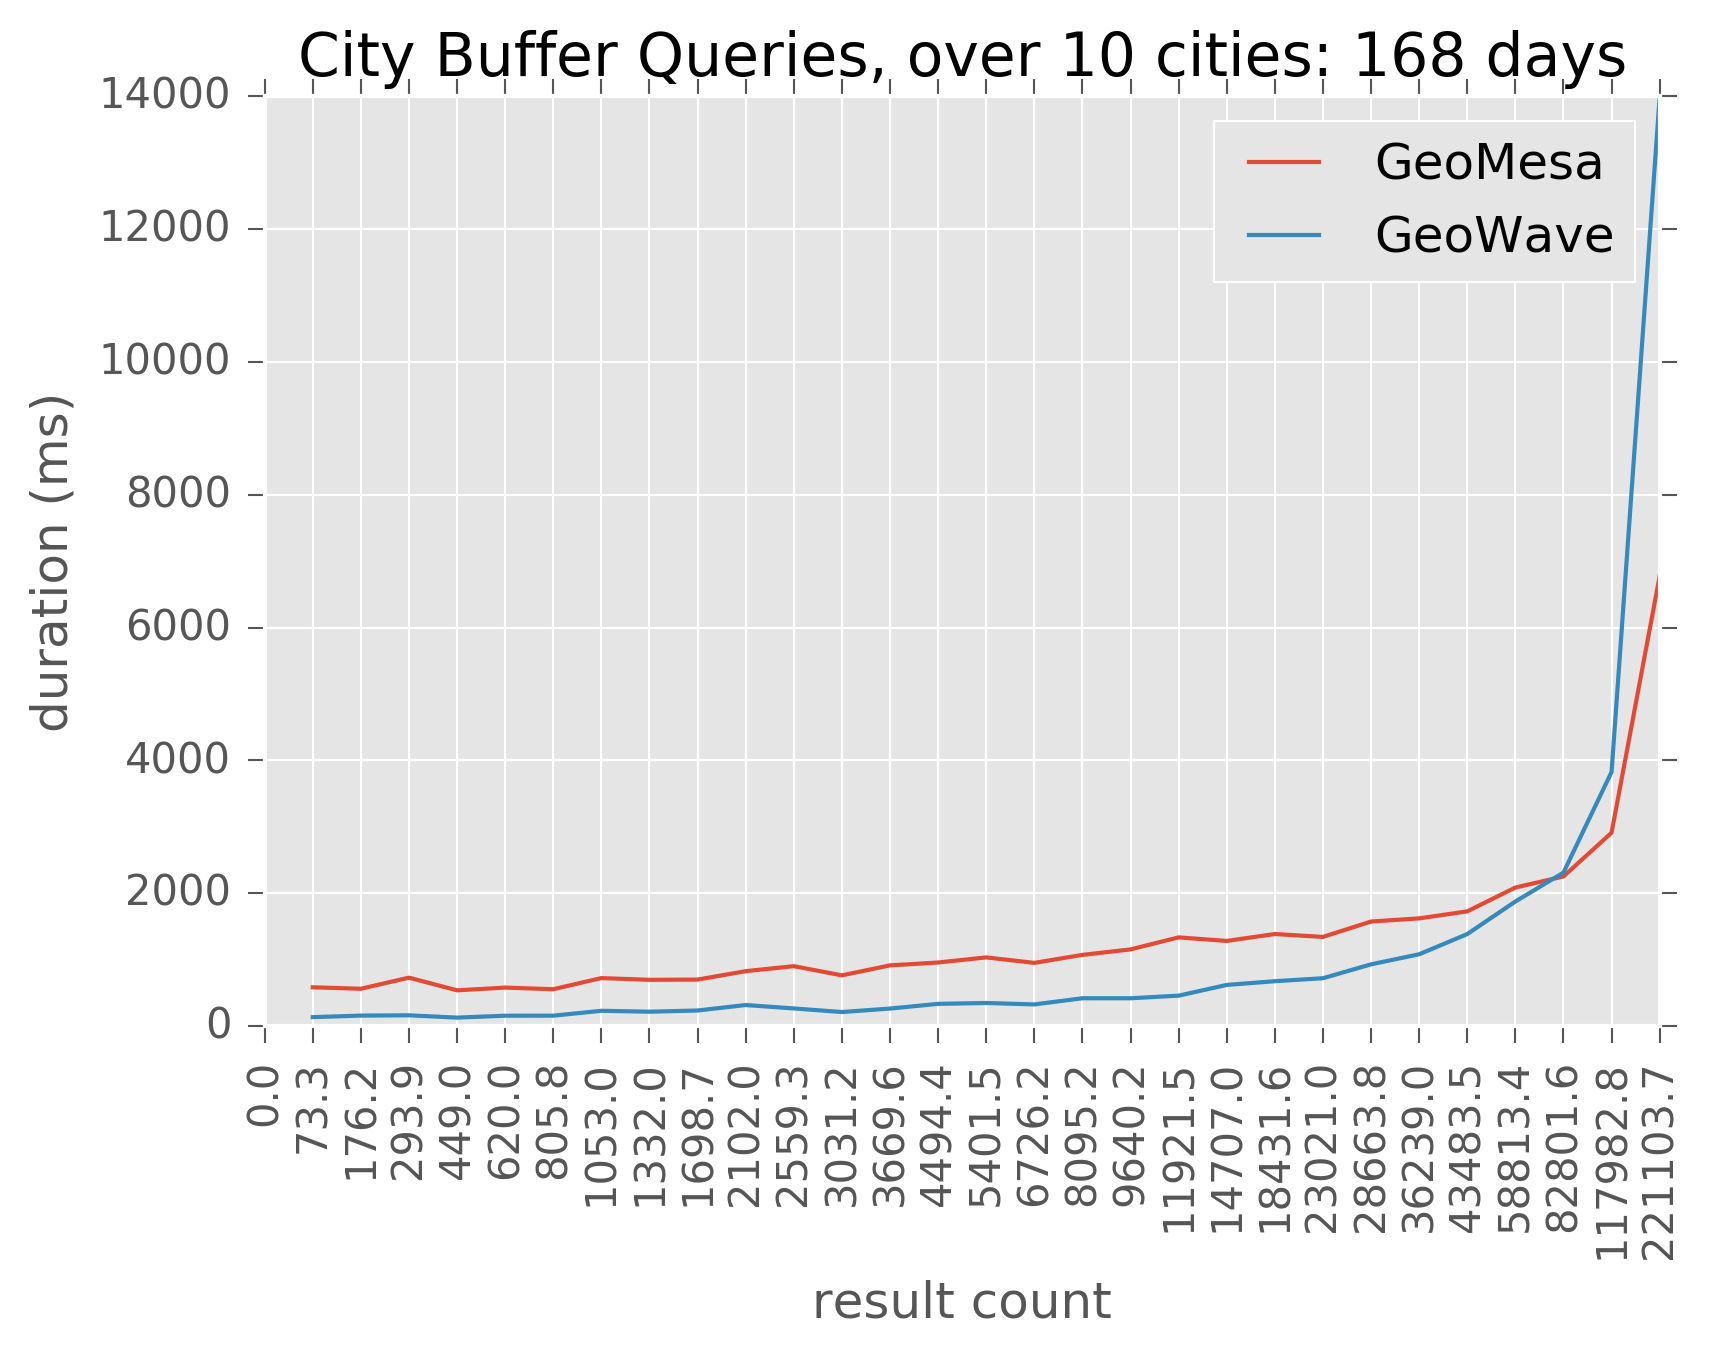
\includegraphics[width=0.60\textwidth]{../docs/img/gdelt/168-days-matching.png}
  \caption{Durations over result counts, matching indexes, all queries of $168$ days.}
  \label{matching168}
\end{figure}

When we look at the overall timings based on result count, we can that GeoMesa seems to be slightly
outperformed by GeoWave until a certain result set size is reached.
Please see Figure \ref{matching}.

\begin{figure}[h!tb]
  \centering
  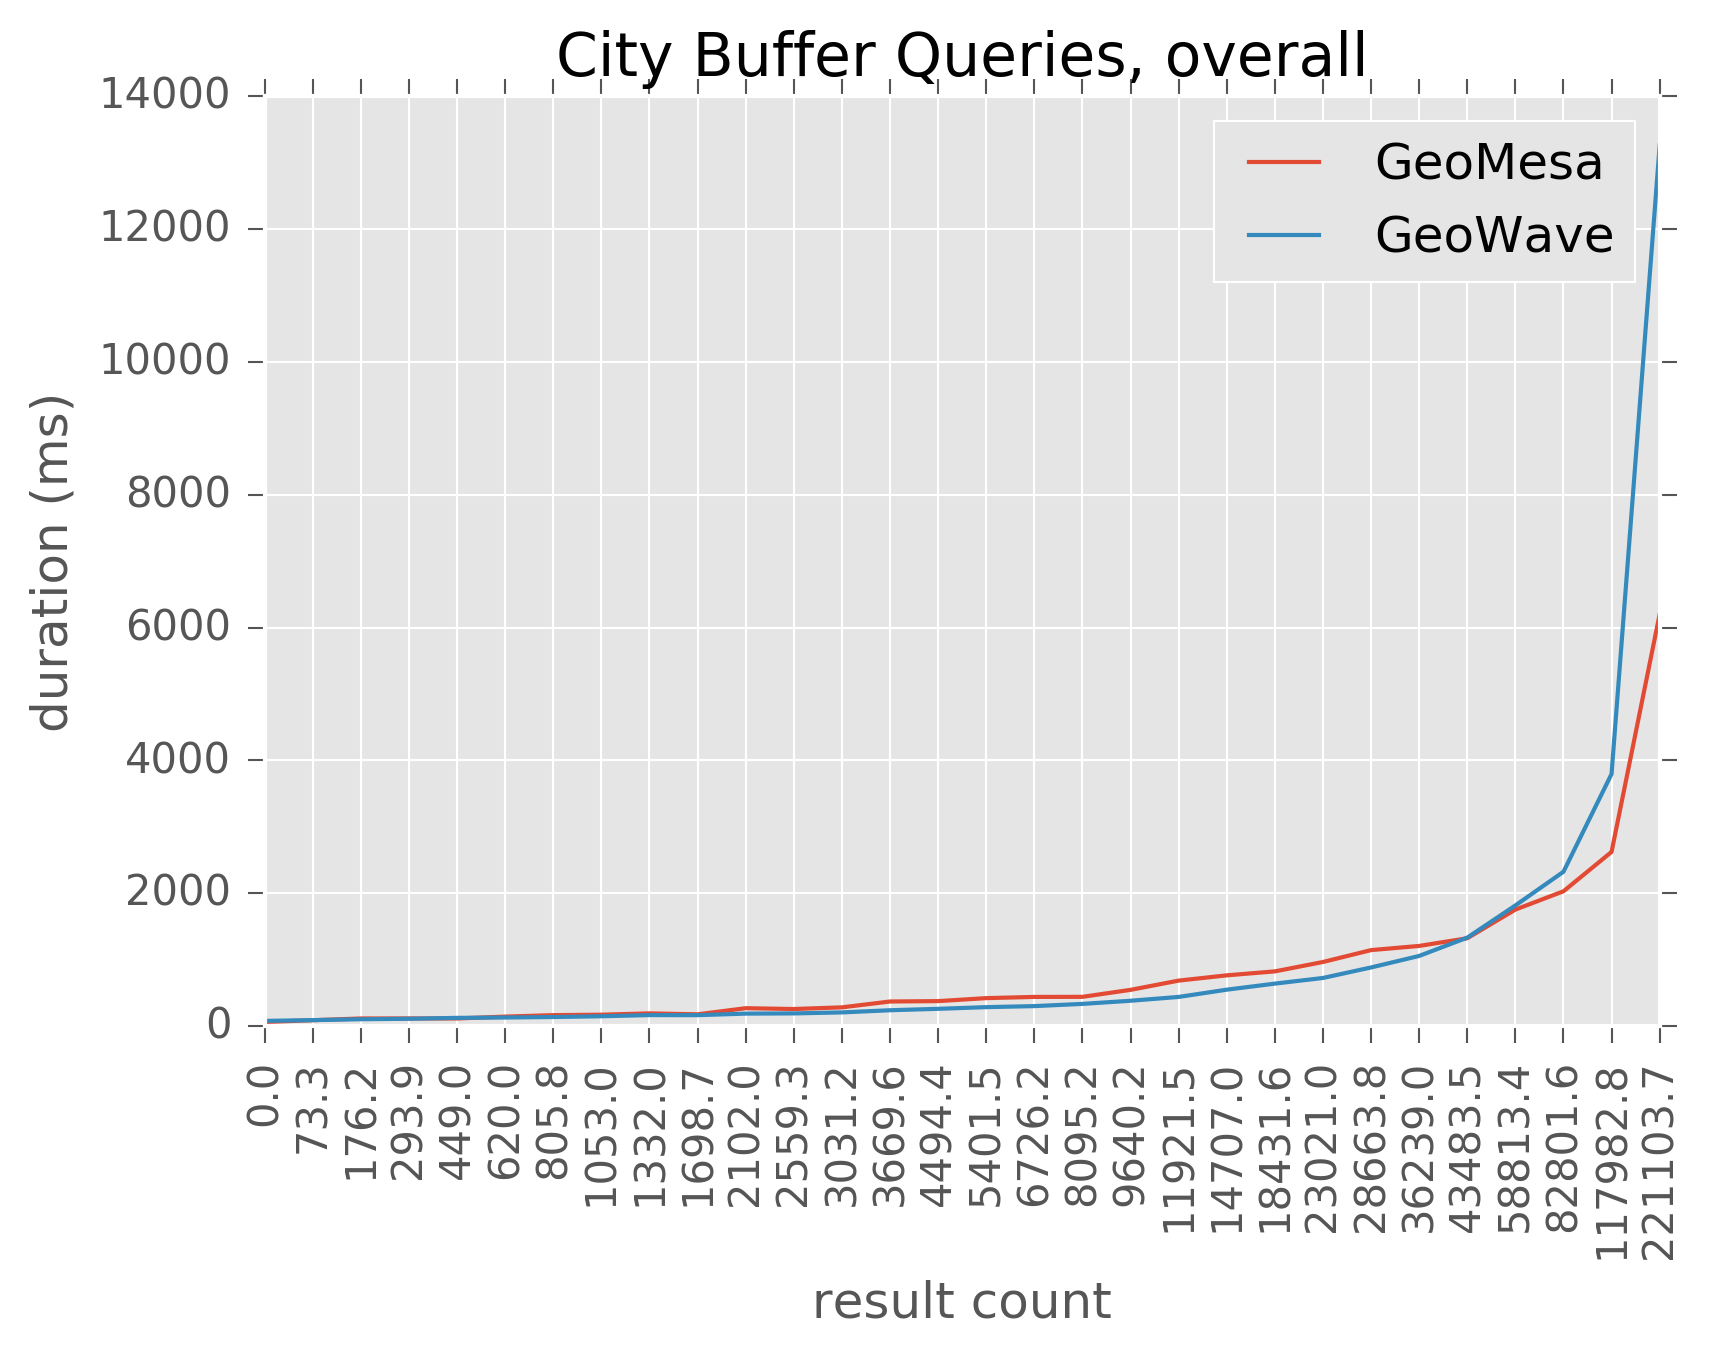
\includegraphics[width=0.60\textwidth]{../docs/img/gdelt/overall-duration-vs-result-matching.png}
  \caption{Durations over result counts, matching, all queries.}
  \label{matching}
\end{figure}

If we focus in on query durations with relatively lower result counts,
and plot GeoMesa and GeoWave results with both the default and the matched index configuration,
we see that both systems improve with the matched index configuration,
and that GeoWave outperforms GeoMesa in this case for both index configurations.
Please see Figure \ref{matchingclamp20}.

%% <!-- ![Durations over result counts, matching, all queries, clamp 20](img/gdelt/overall-duration-vs-result-matching-cap-20.png) -->

\begin{figure}[h!tb]
  \centering
  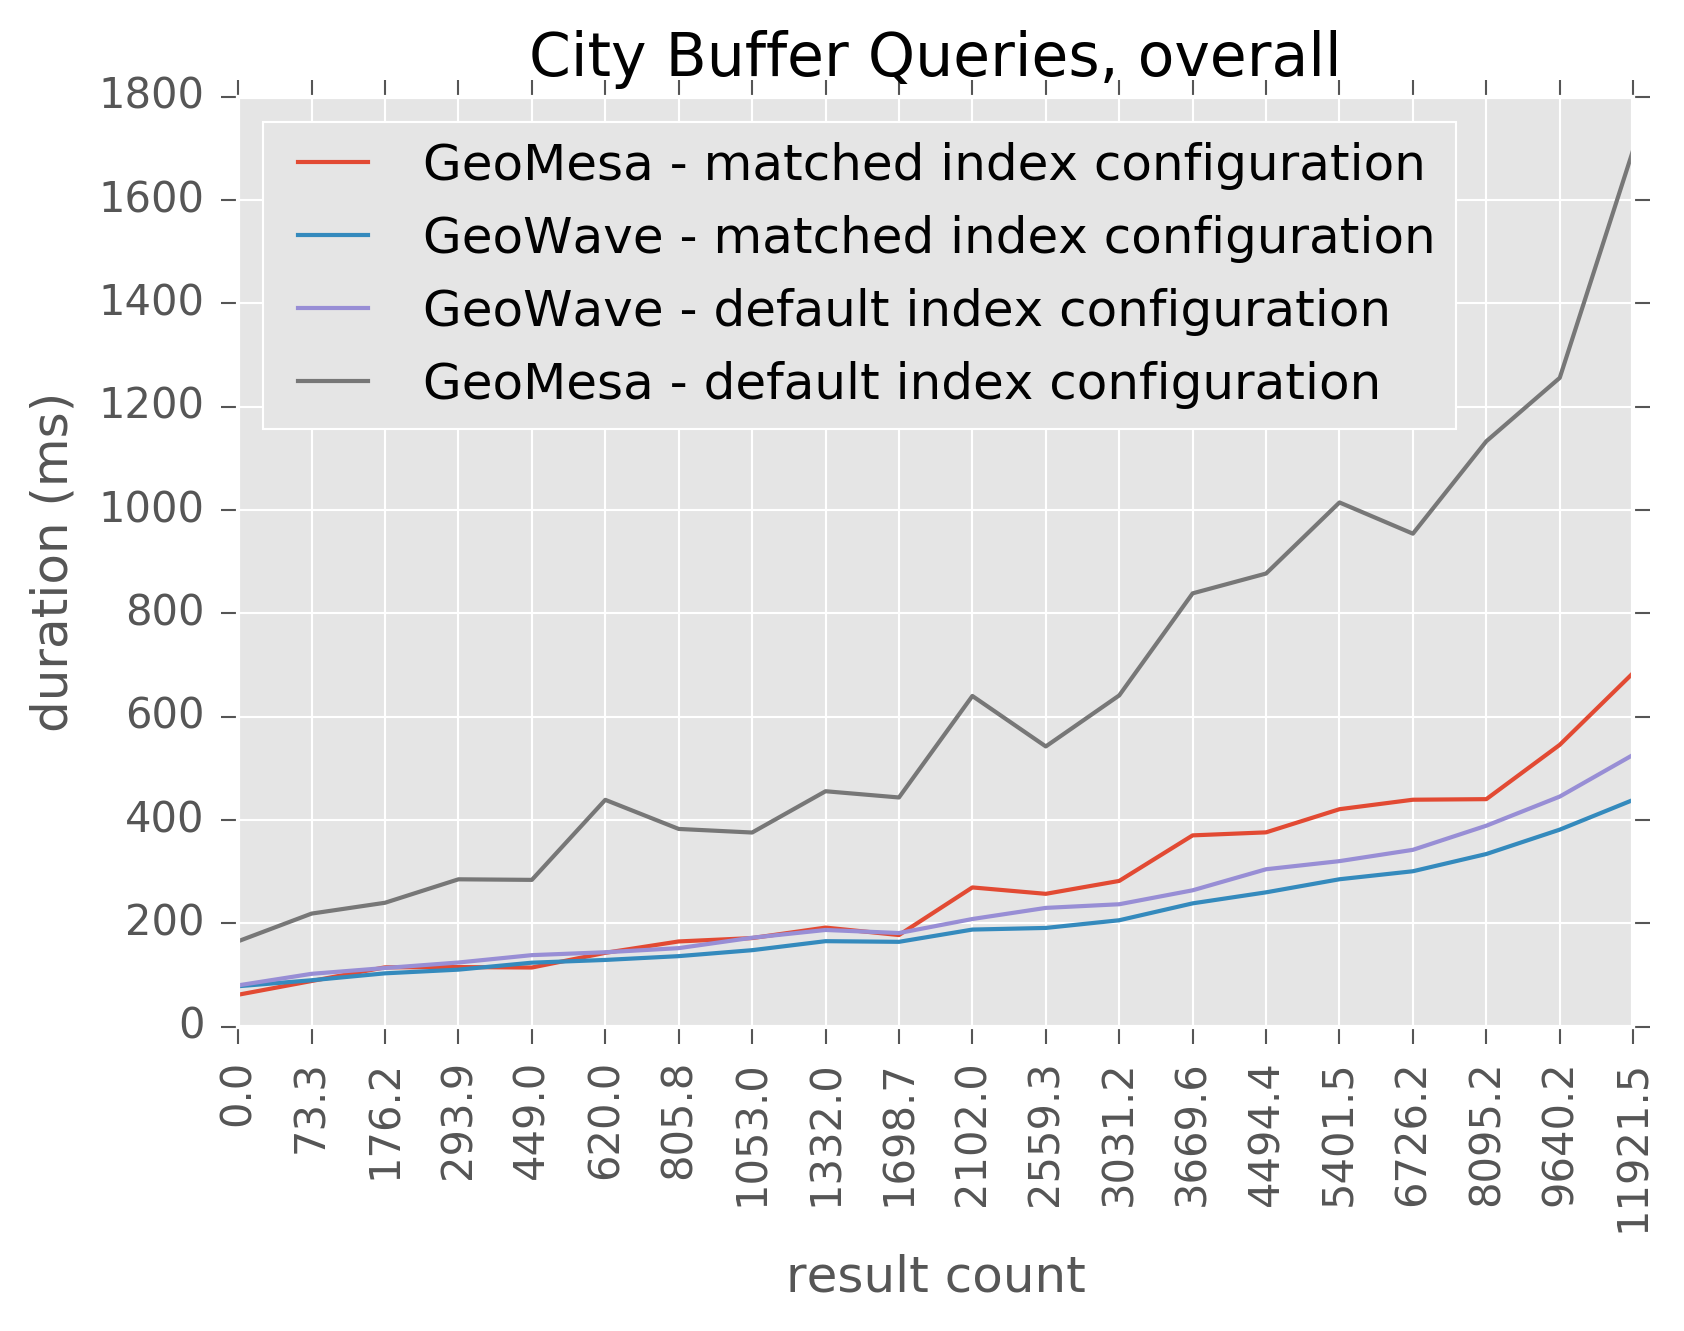
\includegraphics[width=0.60\textwidth]{../docs/img/gdelt/overall-duration-vs-result-both-cap-20.png}
  \caption{Durations over result counts, matching, all queries, clamp $20$.}
  \label{matchingclamp20}
\end{figure}

If we only look at queries with time bounds that are less than 30 days, we see the GeoMesa matched index configuration
performing the best out of that group.
Please see Figure \ref{matchinglt3020}.

\begin{figure}[h!tb]
  \centering
  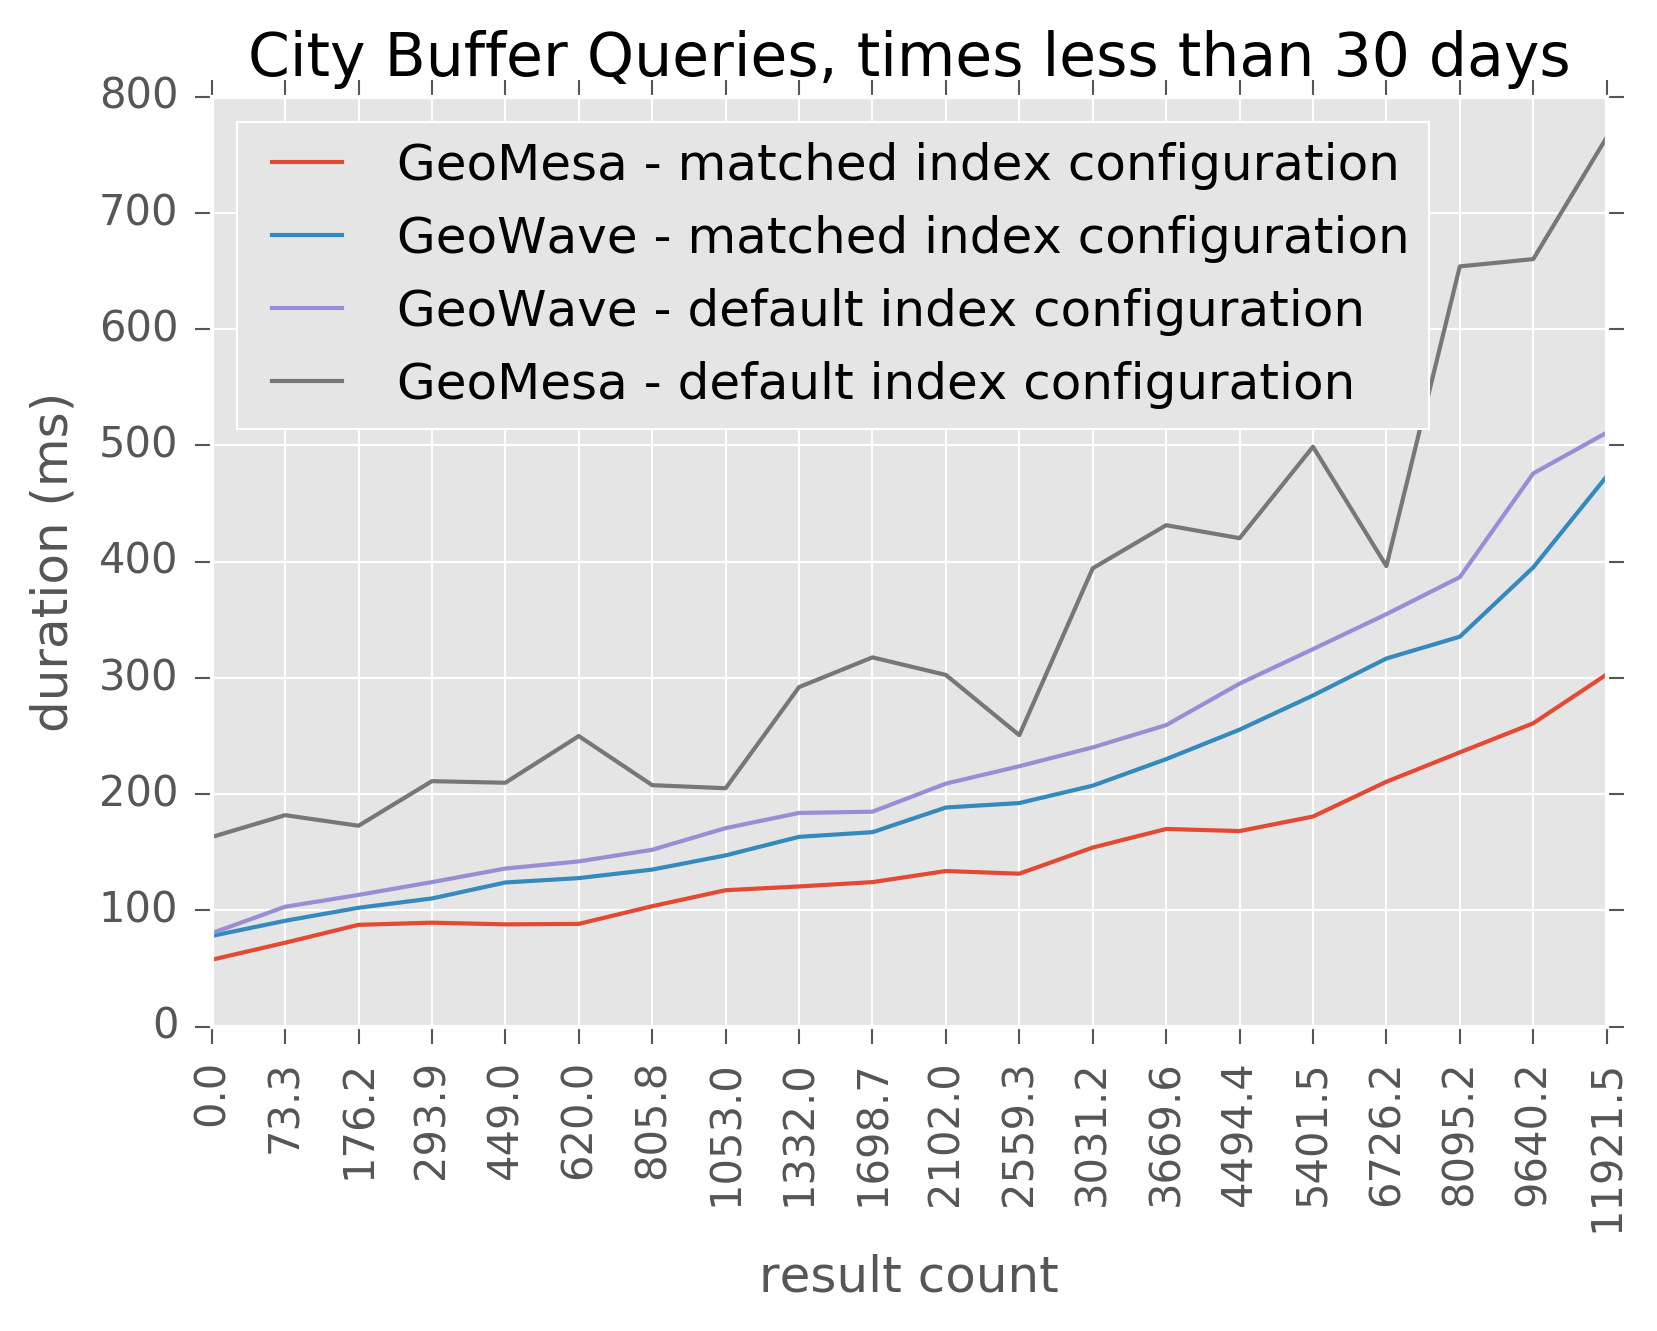
\includegraphics[width=0.60\textwidth]{../docs/img/gdelt/lt-30days-duration-vs-result-both-cap-20.png}
  \caption{Durations over result counts, both, less than $30$ days, clamp $20$.}
  \label{matchinglt3020}
\end{figure}

When we only consider queries over 30 days, we see a more marked advantage of GeoWave performance.
Please see Figure \ref{matchinggt3020}.

\begin{figure}[h!tb]
  \centering
  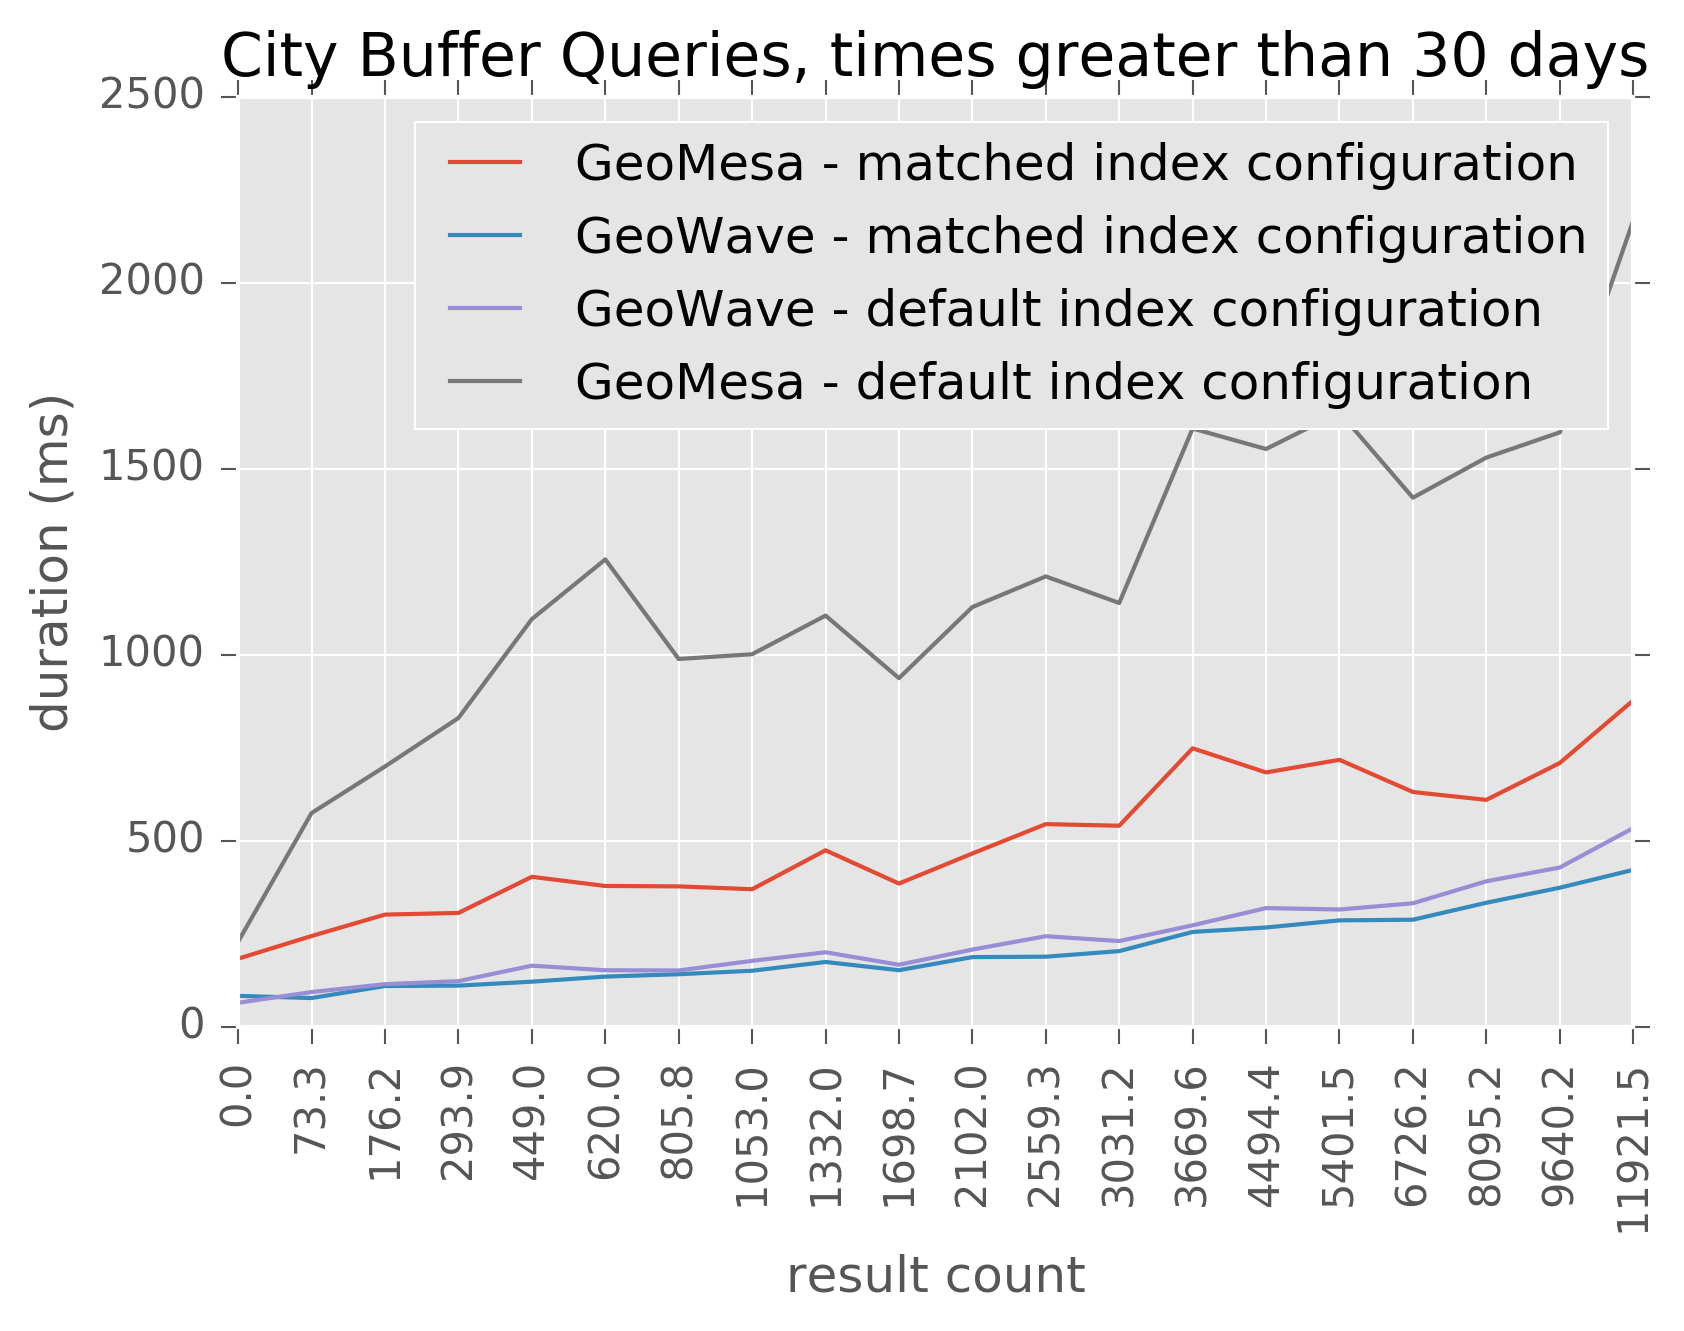
\includegraphics[width=0.60\textwidth]{../docs/img/gdelt/gt-30days-duration-vs-result-both-cap-20.png}
  \caption{Durations over result counts, both, greater than $30$ days, clamp $20$.}
  \label{matchinggt3020}
\end{figure}

%% <!-- ![Durations over result counts, both, less than 30 days](img/gdelt/lt-30days-duration-vs-result-both.png) -->
%% <!-- ![Durations over result counts, both, greater than 30 days](img/gdelt/gt-30days-duration-vs-result-both.png) -->

Here is the duration of queries plotted over the temporal bounds of the query.
We see that GeoMesa performs better for queries with a small time window,
and both GeoMesa and GeoWave show better performance with the matched index configuration.
Please see Figure \ref{durationdaysboth}.

\begin{figure}[h!tb]
  \centering
  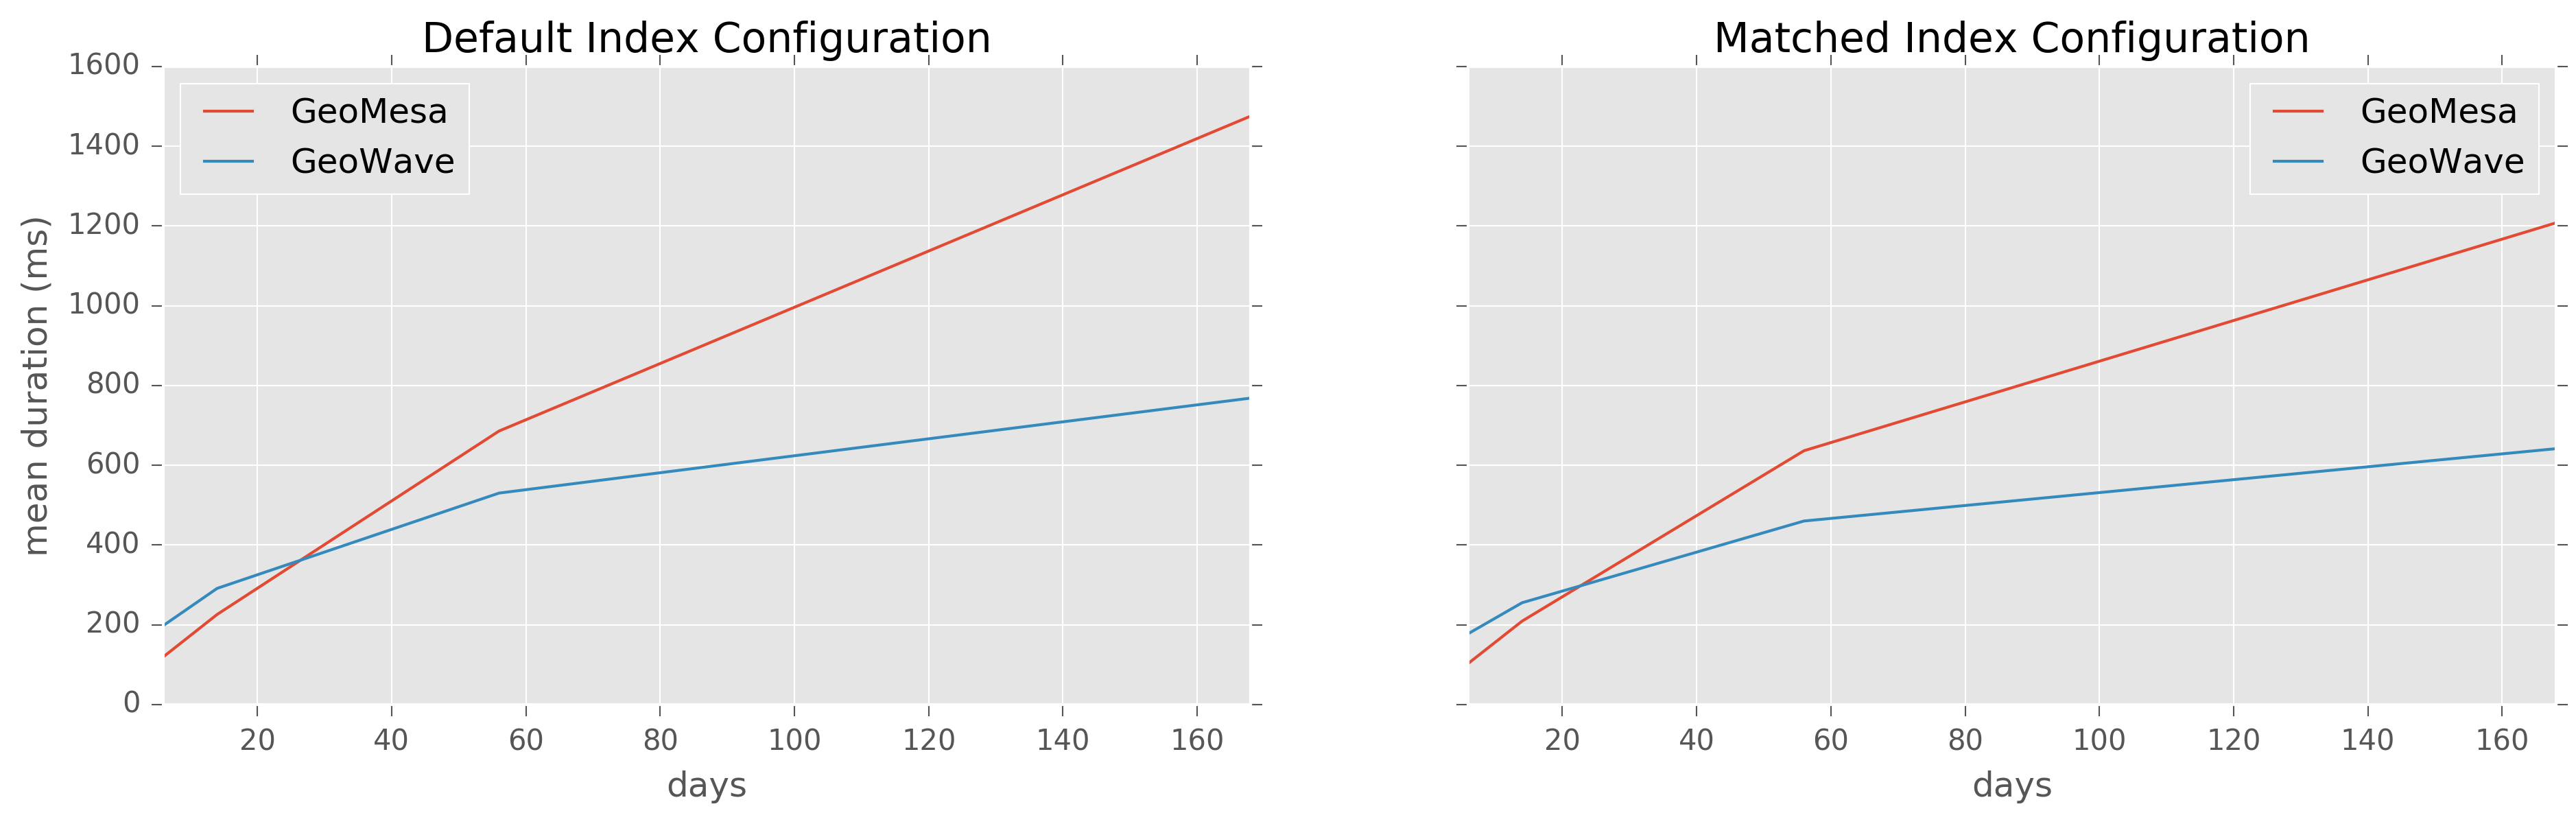
\includegraphics[width=0.60\textwidth]{../docs/img/gdelt/duration-over-days-default-and-matching.png}
  \caption{Durations over days, both.}
  \label{durationdaysboth}
\end{figure}

Looking at the data in another way, we see that the size of the spatial component of the query
(shown in the $x$-axis here in kilometers)
does not have the same threshold-crossing effect as the temporal component does,
and that on average GeoWave outperforms GeoMesa across spatial queries.
Please see Figure \ref{durationsize}.

\begin{figure}[h!tb]
  \centering
  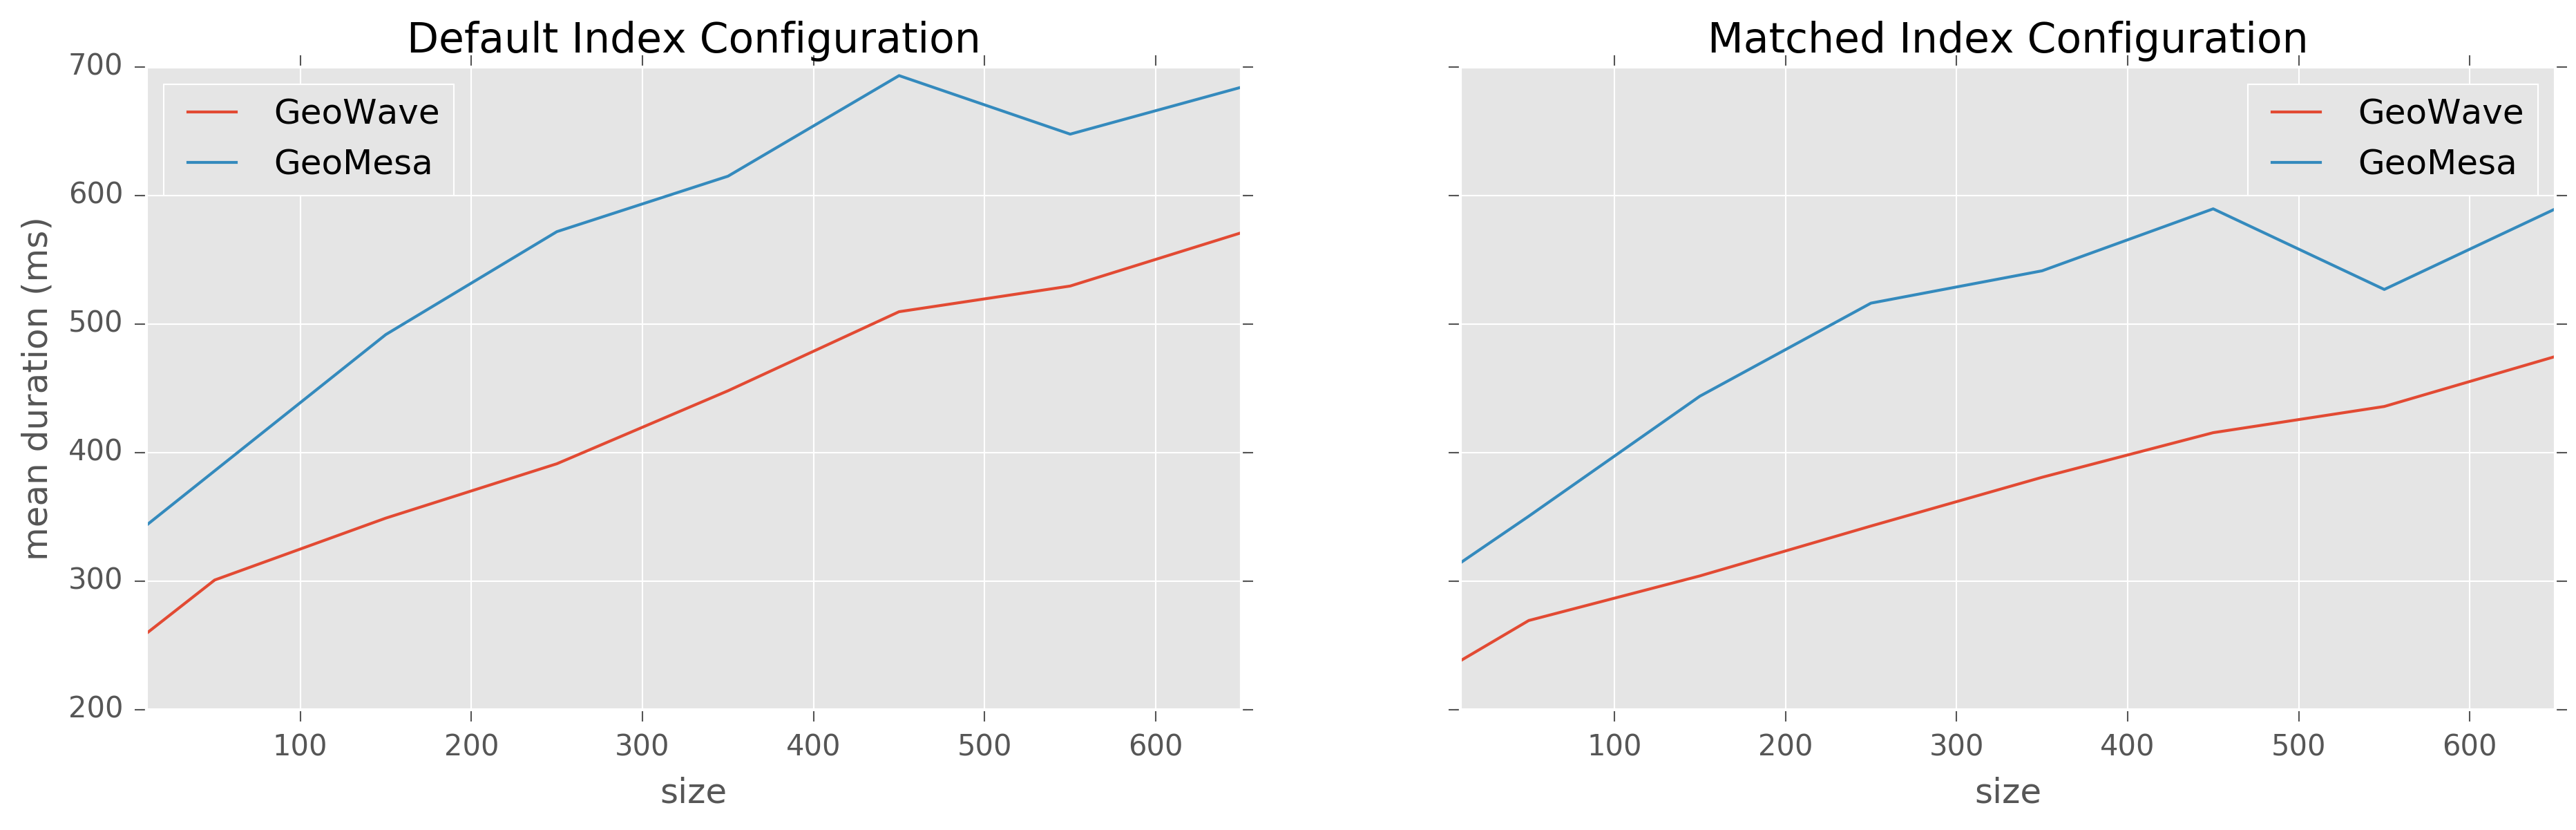
\includegraphics[width=0.60\textwidth]{../docs/img/gdelt/duration-over-size-default-and-matching.png}
  \caption{Durations over days, both.}
  \label{durationsize}
\end{figure}

Finally for the City Buffer tests, we look at how the scatterplot and regression
of durations over result counts changes between the default and the matched index configuration.
Please see Figure \ref{durationresult}.

\begin{figure}[h!tb]
  \centering
  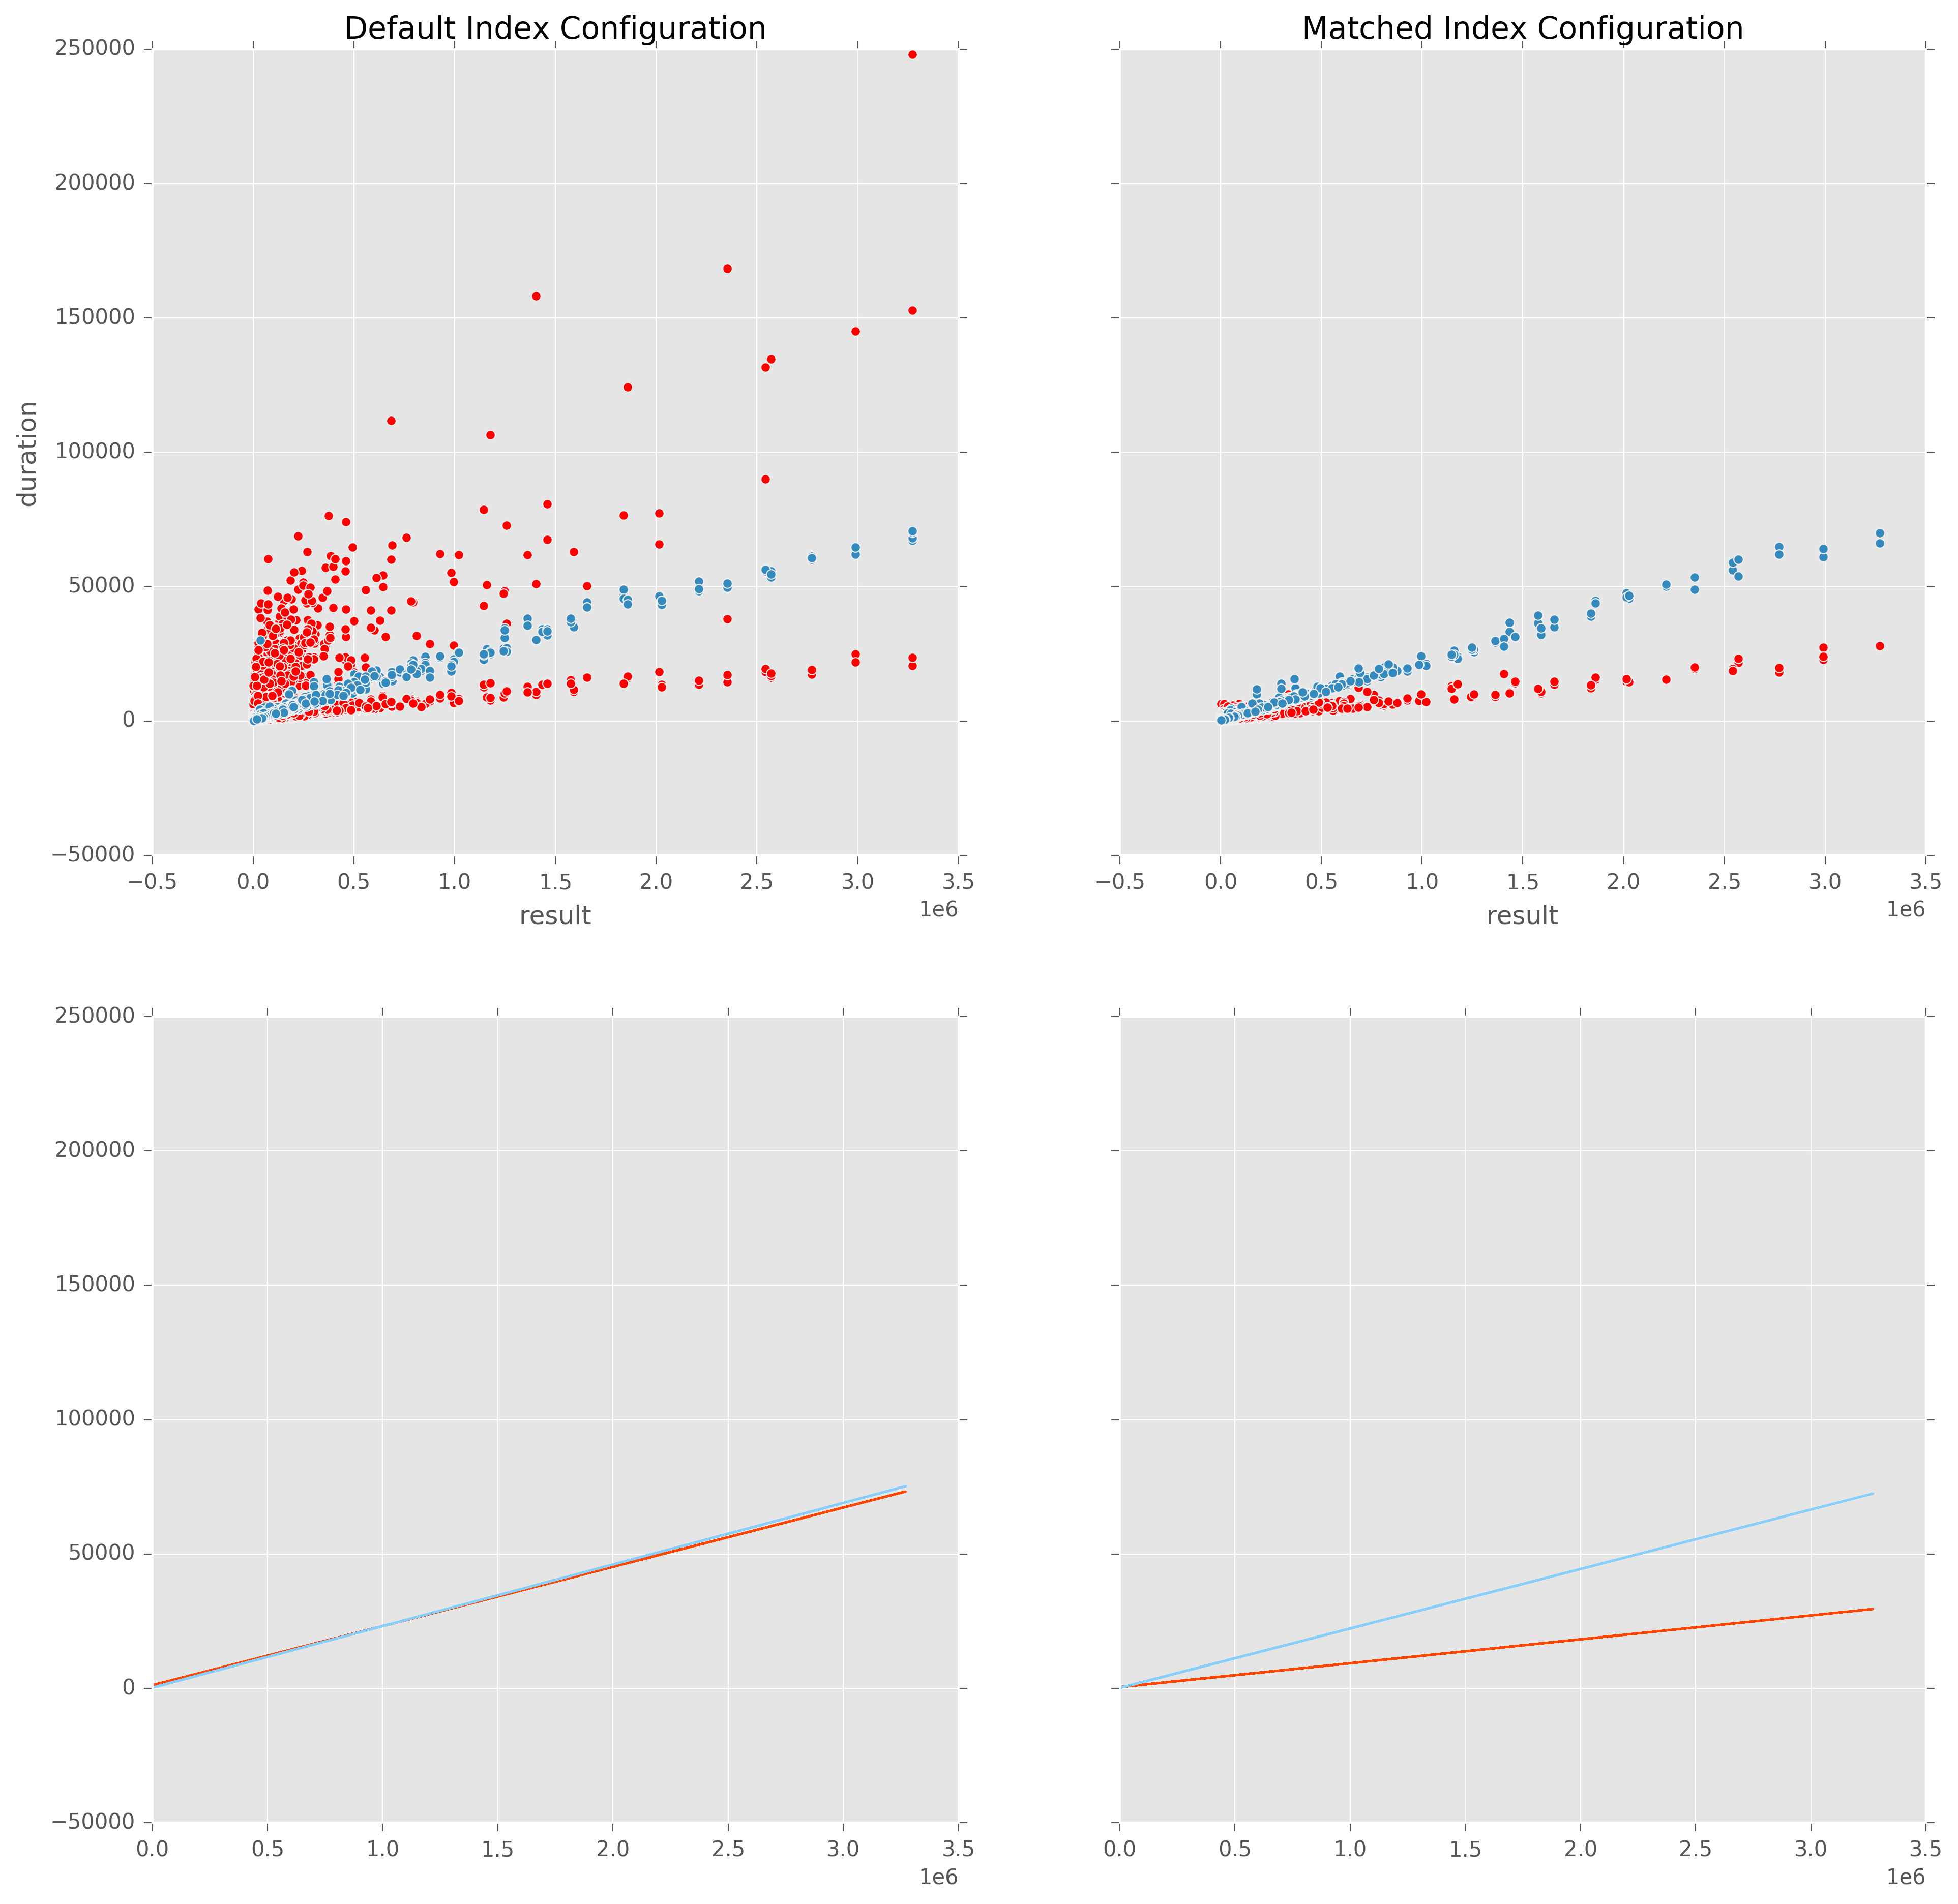
\includegraphics[width=0.60\textwidth]{../docs/img/gdelt/duration-over-result-default-and-matching.png}
  \caption{Durations over result, scatter and regression, both.}
  \label{durationresult}
\end{figure}

\subsubsection{South America}

We queried events within South American countries (Figure \ref{southamerica})
for three weeks of every month of every year from 2000 to 2016.

\begin{figure}[h!tb]
  \centering
  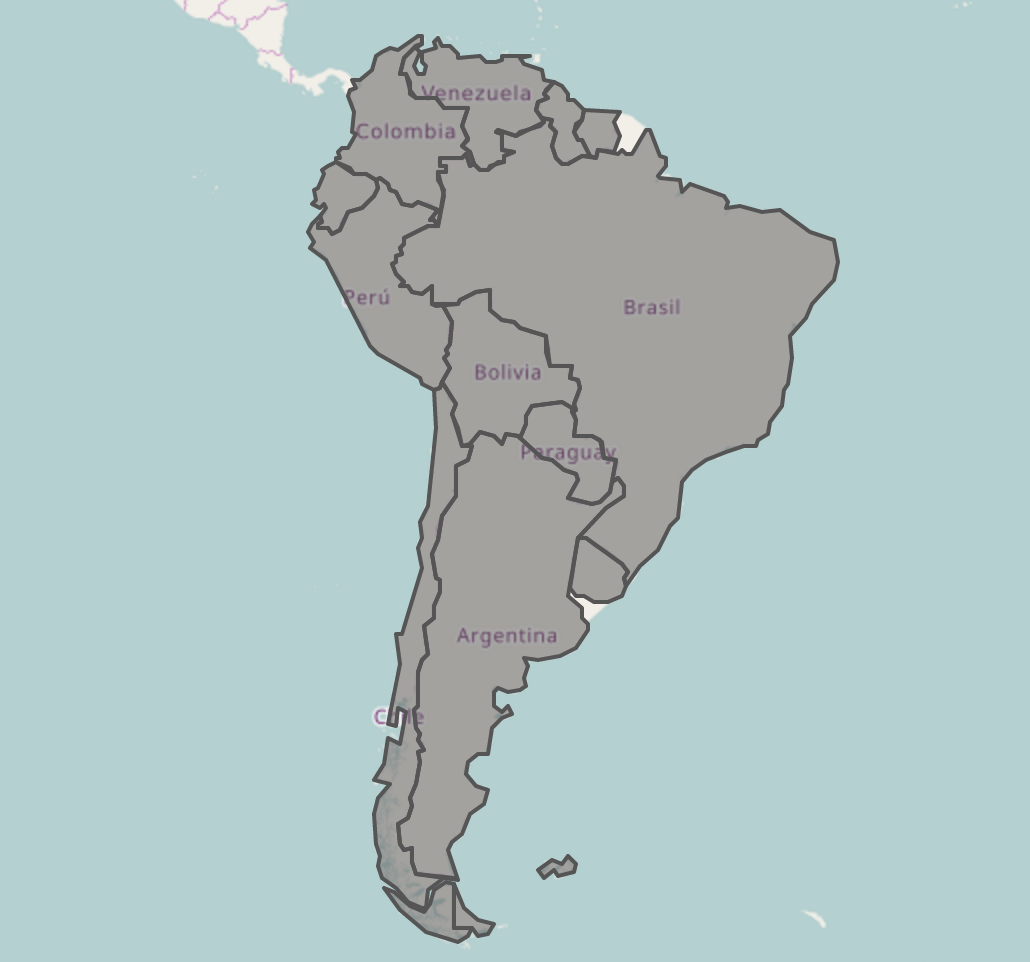
\includegraphics[width=0.60\textwidth]{../docs/img/gdelt/south-america-countries.png}
  \caption{South America.}
  \label{southamerica}
\end{figure}

The results we found for this area of the world were unsurprising,
with the matching index configuration performing better in both systems than the default index configuration,
and the effect of result count having a greater effect on GeoWave performance than GeoMesa.
Figure \ref{sadurations} is a chart is of the duration of query execution over result size, with outliers removed.

\begin{figure}[h!tb]
  \centering
  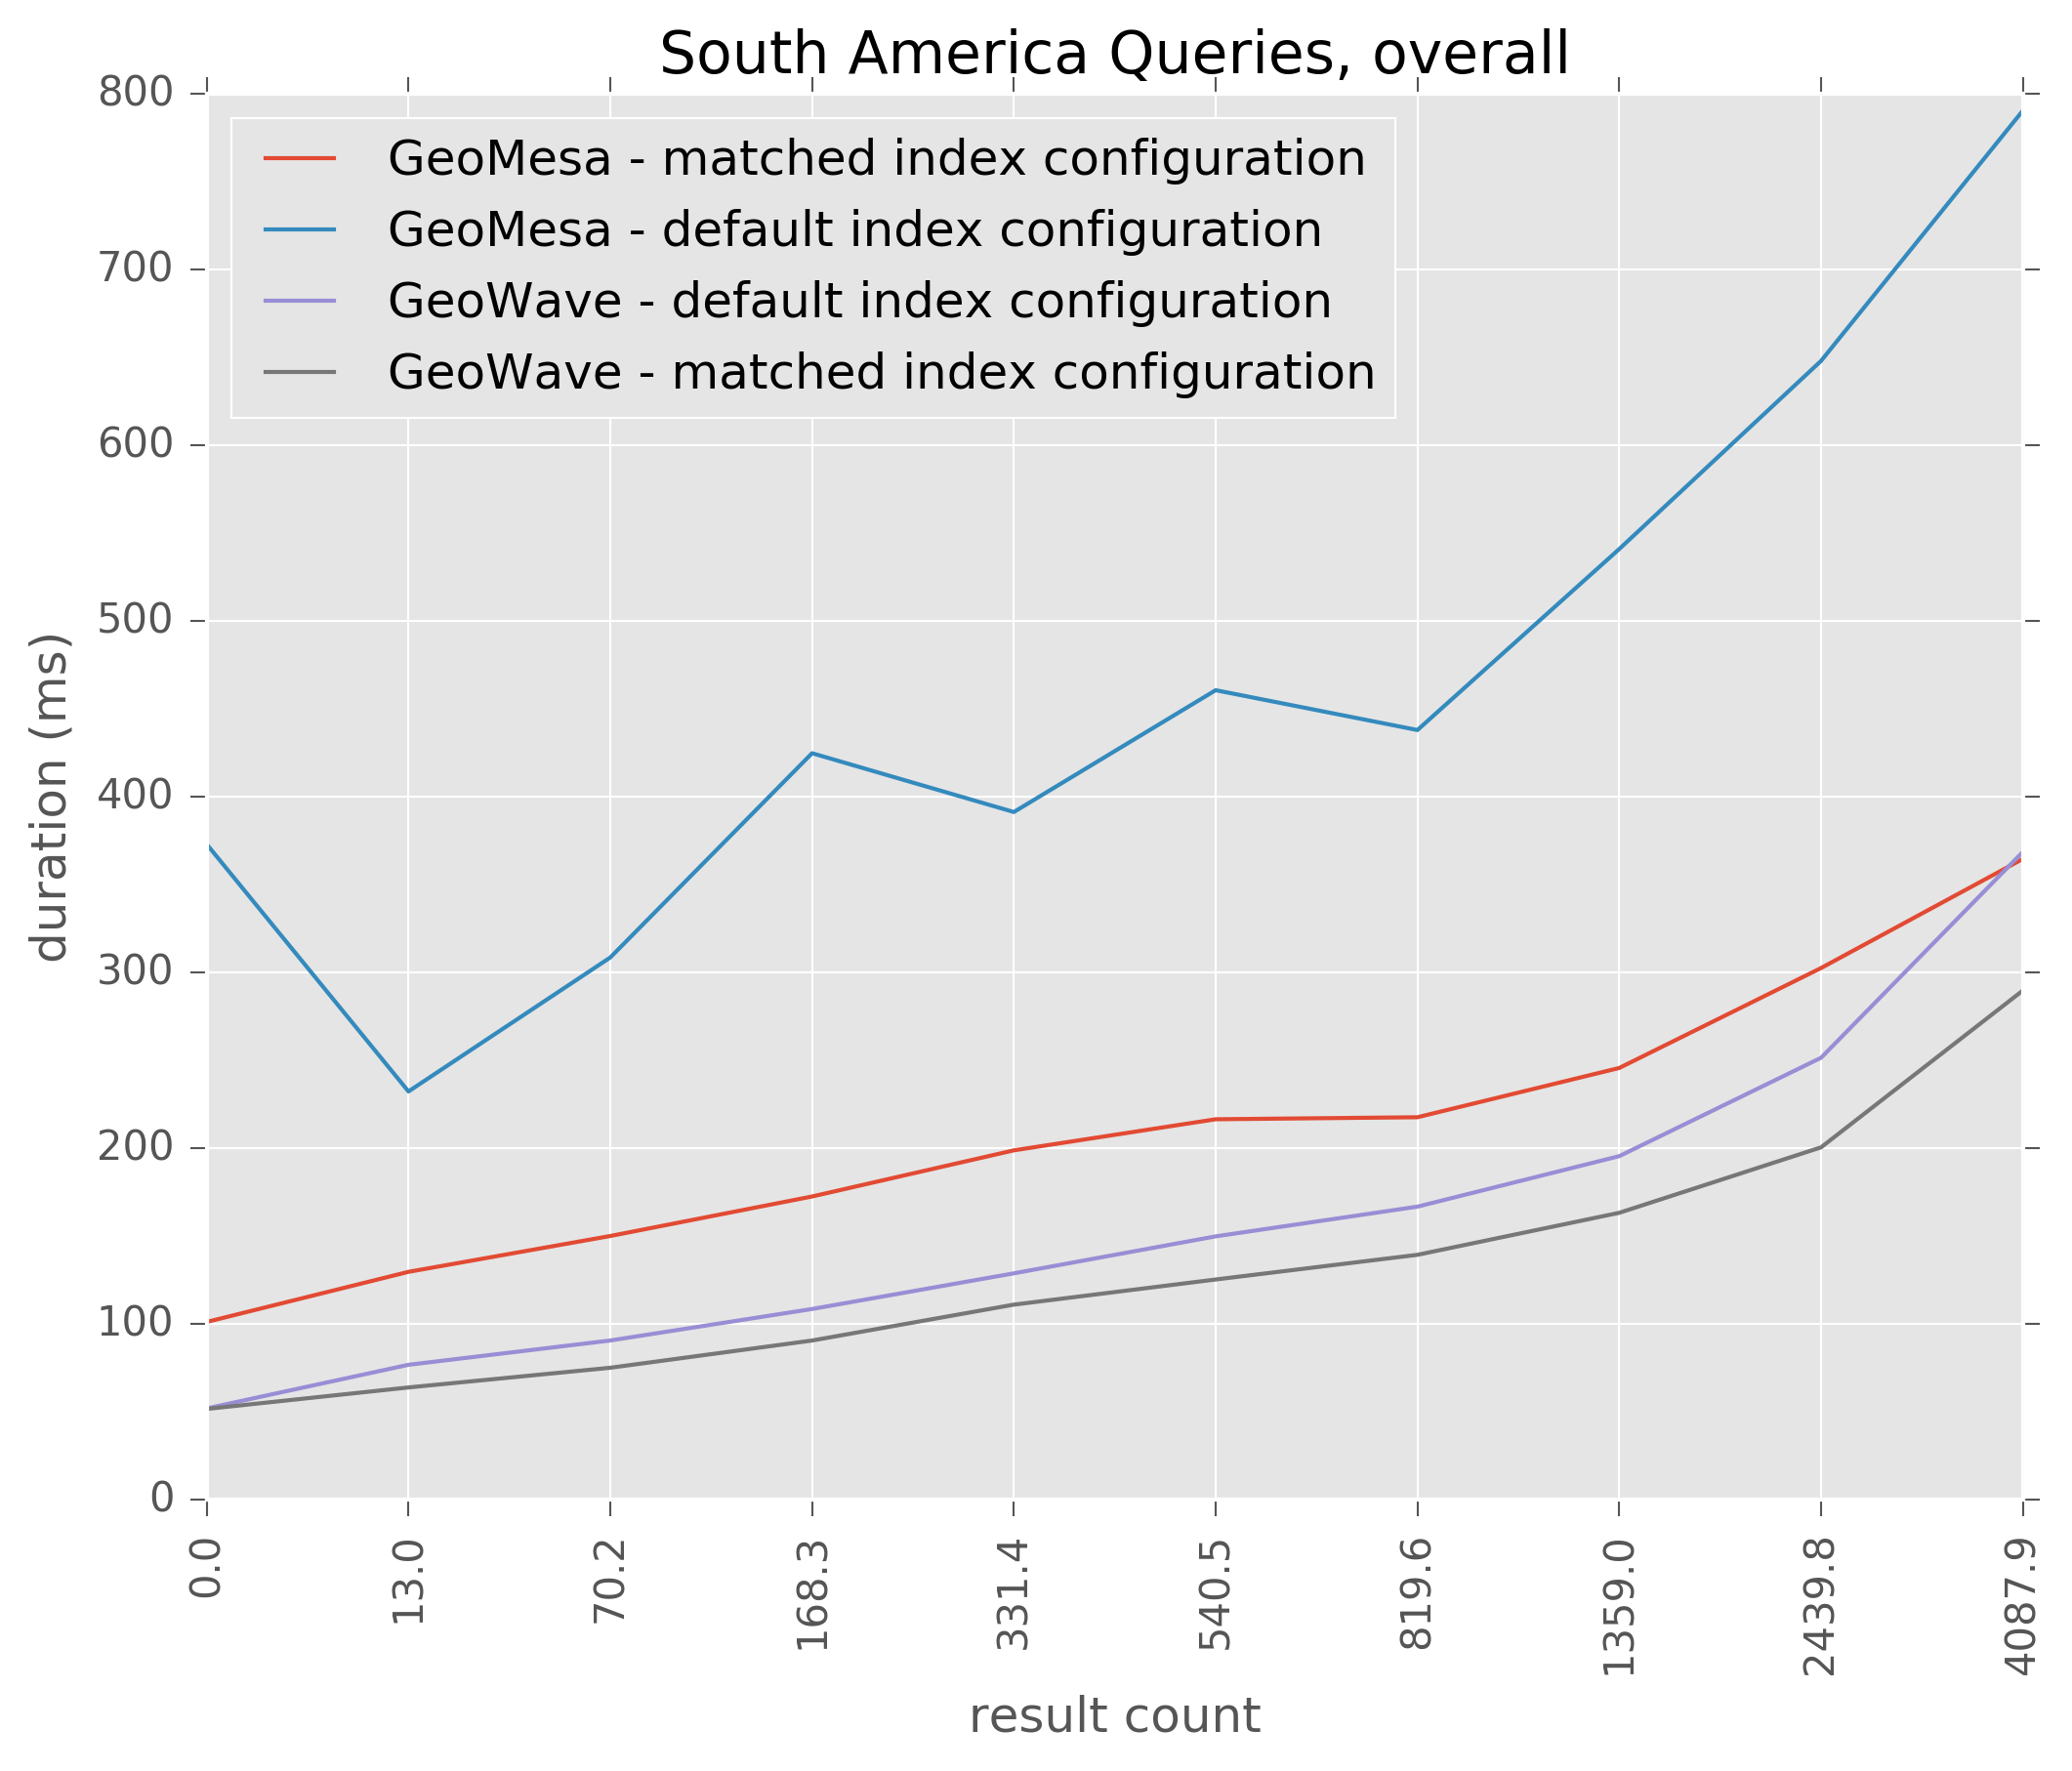
\includegraphics[width=0.60\textwidth]{../docs/img/gdelt/sa-overall-duration-vs-result-both.png}
  \caption{Durations over result counts, both, all queries.}
  \label{sadurations}
\end{figure}


\subsection{Synthesized Tracks}

Test for Tracks data were performed on EMR 5.0.0 clusters of one \texttt{m3.2xlarge} master and three \texttt{m3.2xlarge} workers.

We performed queries against a range of bounding boxes over the continental United States of America.
We project a powers of $2$ pyramid over this area and query from pyramid level $4$ to $7$,
with temporal bounds being one of $5$ days, $18$ days, $27$ days, or one month.
The beginning of the temporal bounds was selected from the range of time for which data existed.

We refer to the spatial aspect of the bounding box queries according to ``levels'',
where each level refers to a powers of $2$ pyramid over the bounding box of the US.
Figure \ref{tracks} contains a depiction of those bounding boxes, to give a sense of scale.

\begin{figure}[h!tb]
  \centering
  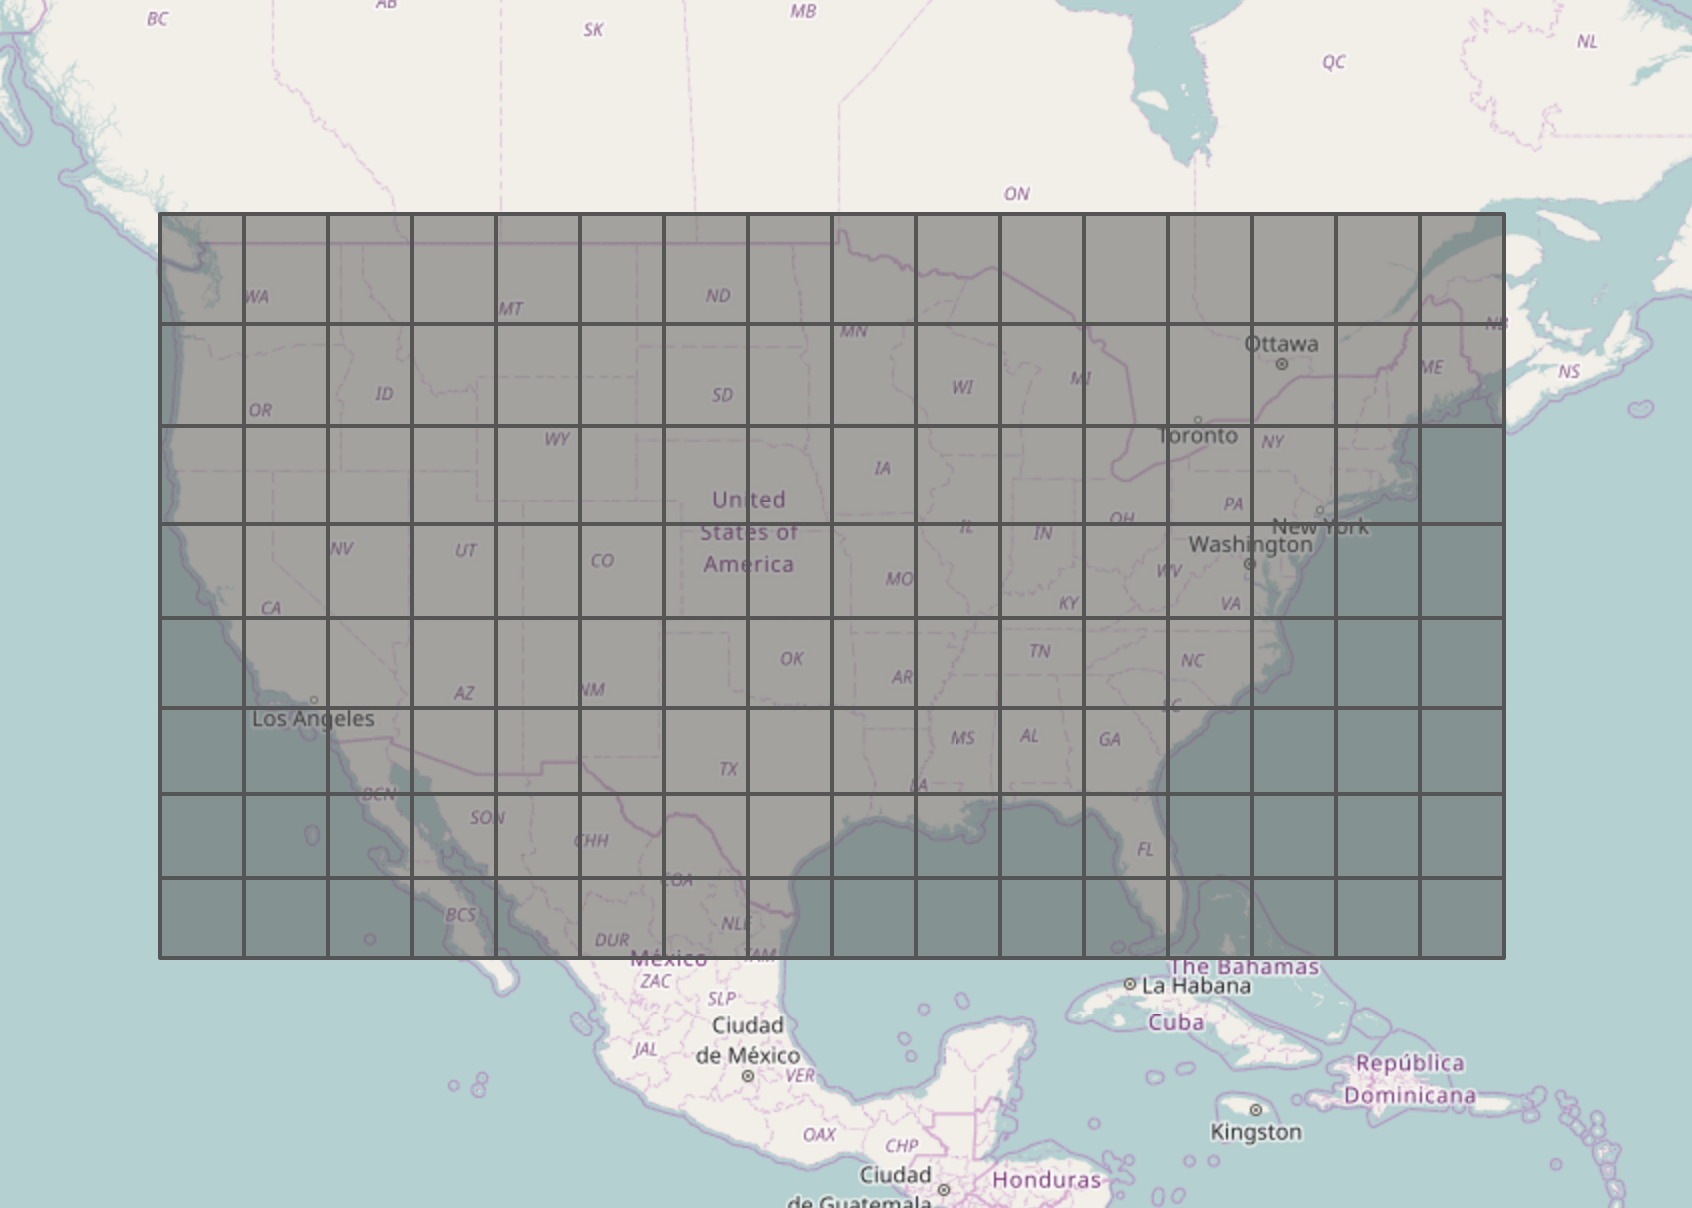
\includegraphics[width=0.45\textwidth]{../docs/img/tracks-usa-grid-4.png}
  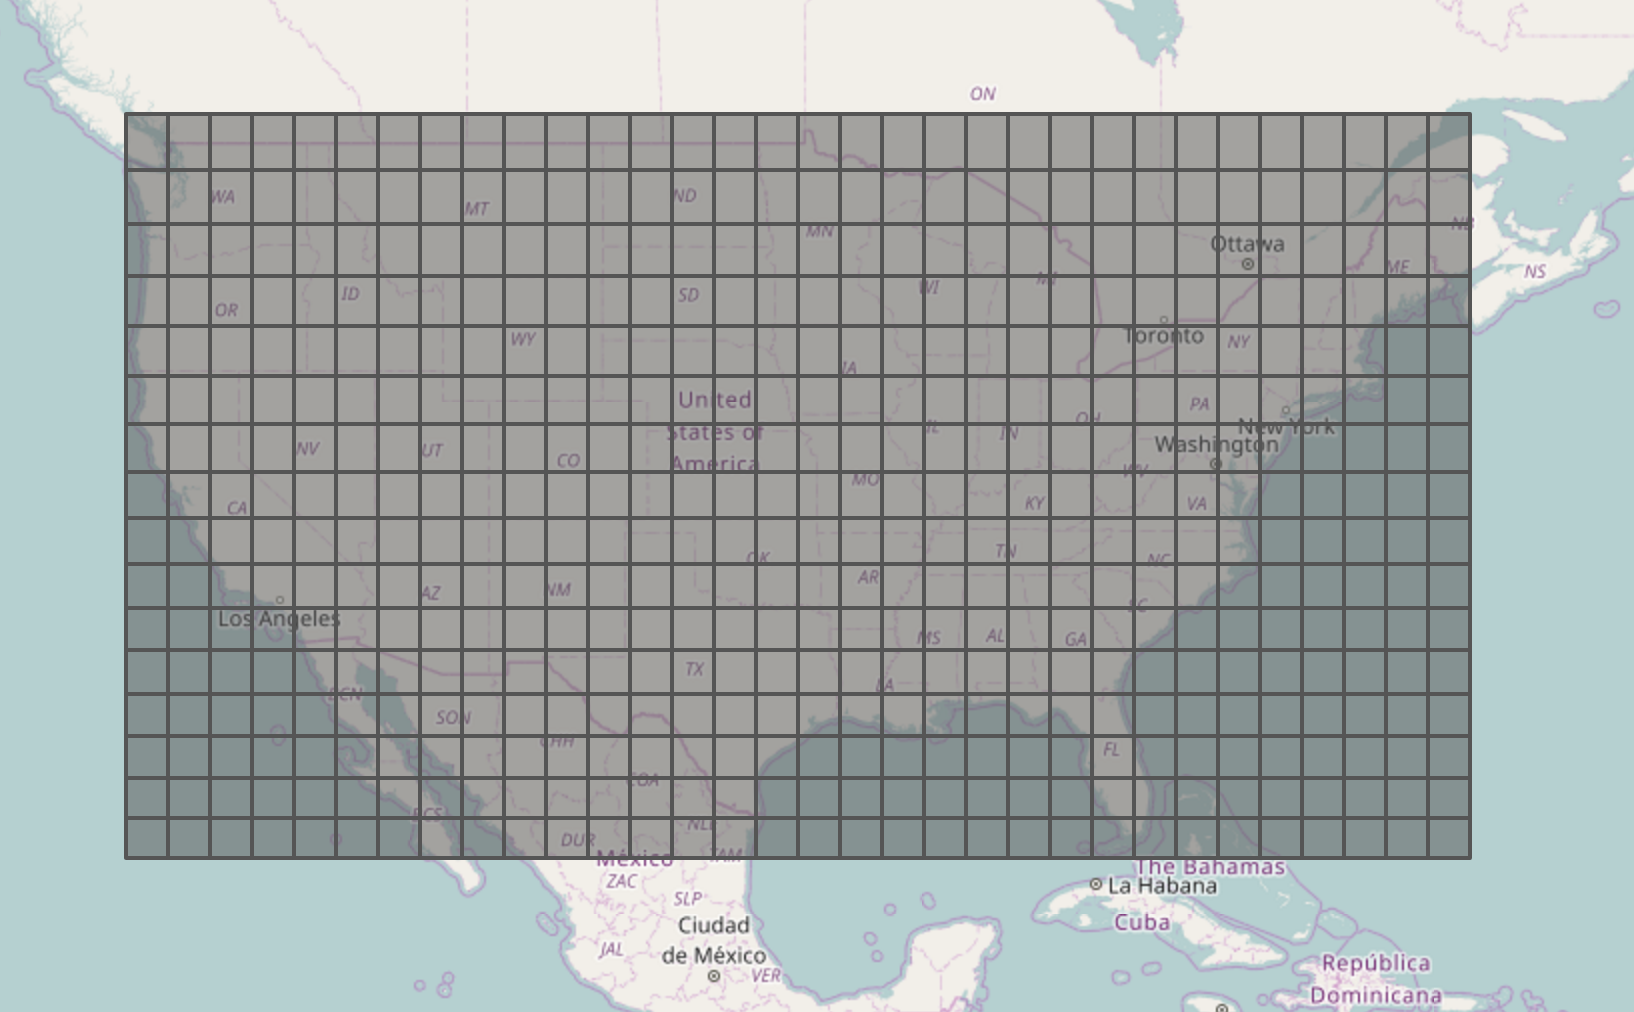
\includegraphics[width=0.45\textwidth]{../docs/img/tracks-usa-grid-5.png}
  \newline
  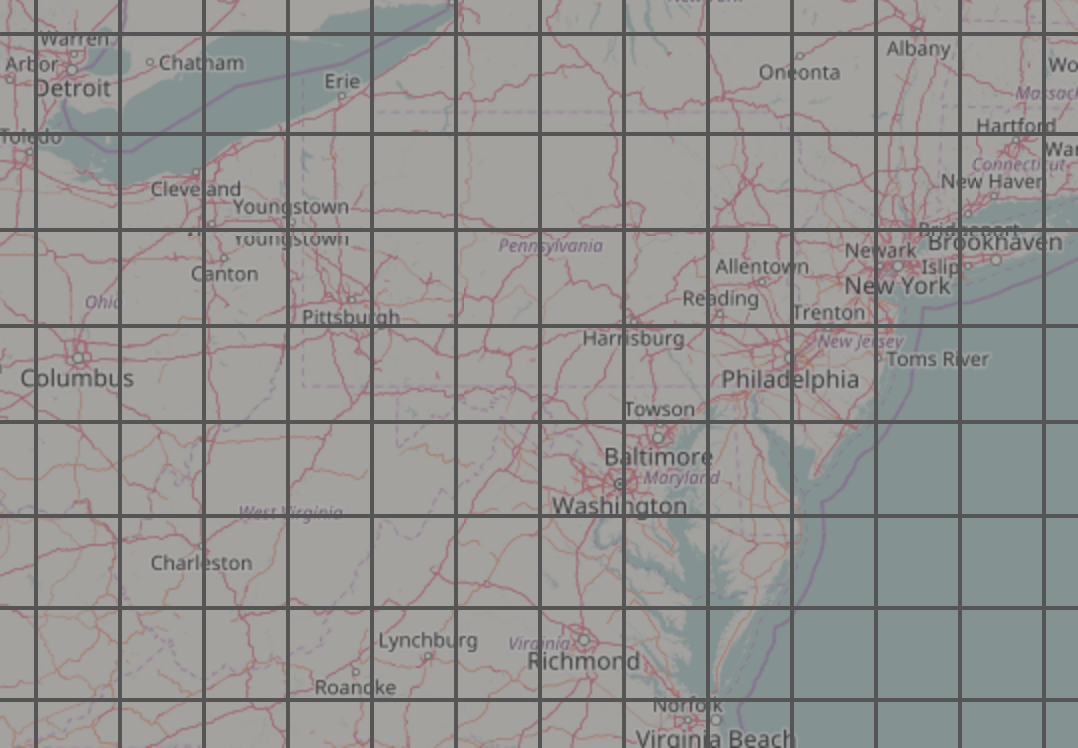
\includegraphics[width=0.45\textwidth]{../docs/img/tracks-usa-grid-6.png}
  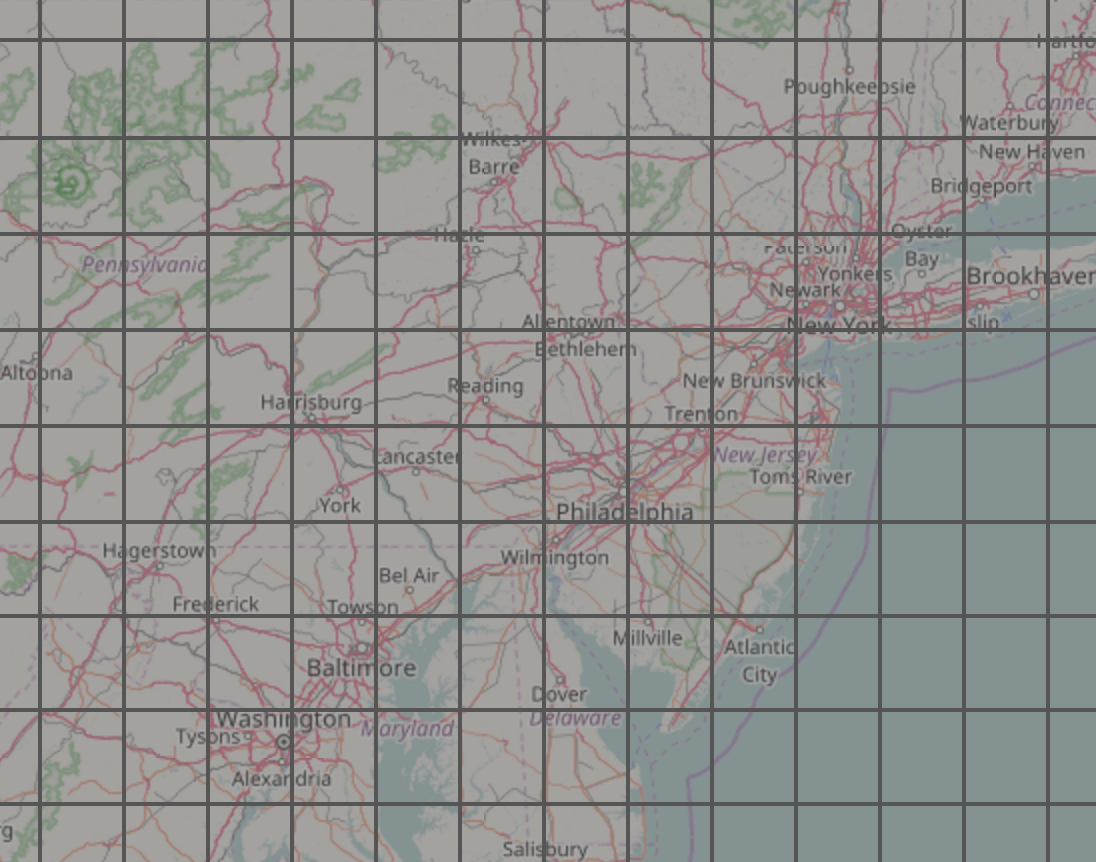
\includegraphics[width=0.45\textwidth]{../docs/img/tracks-usa-grid-7.png}
  \caption{Tracks grids levels $4$, $5$, $6$, and $7$.}
  \label{tracks}
\end{figure}

There is an pattern of behavior exhibited by the query results for the generated tracks dataset that bears some mention.
Consider Figures \ref{tracksgm} and \ref{tracksgw}.

\begin{figure}[h!tb]
  \centering
  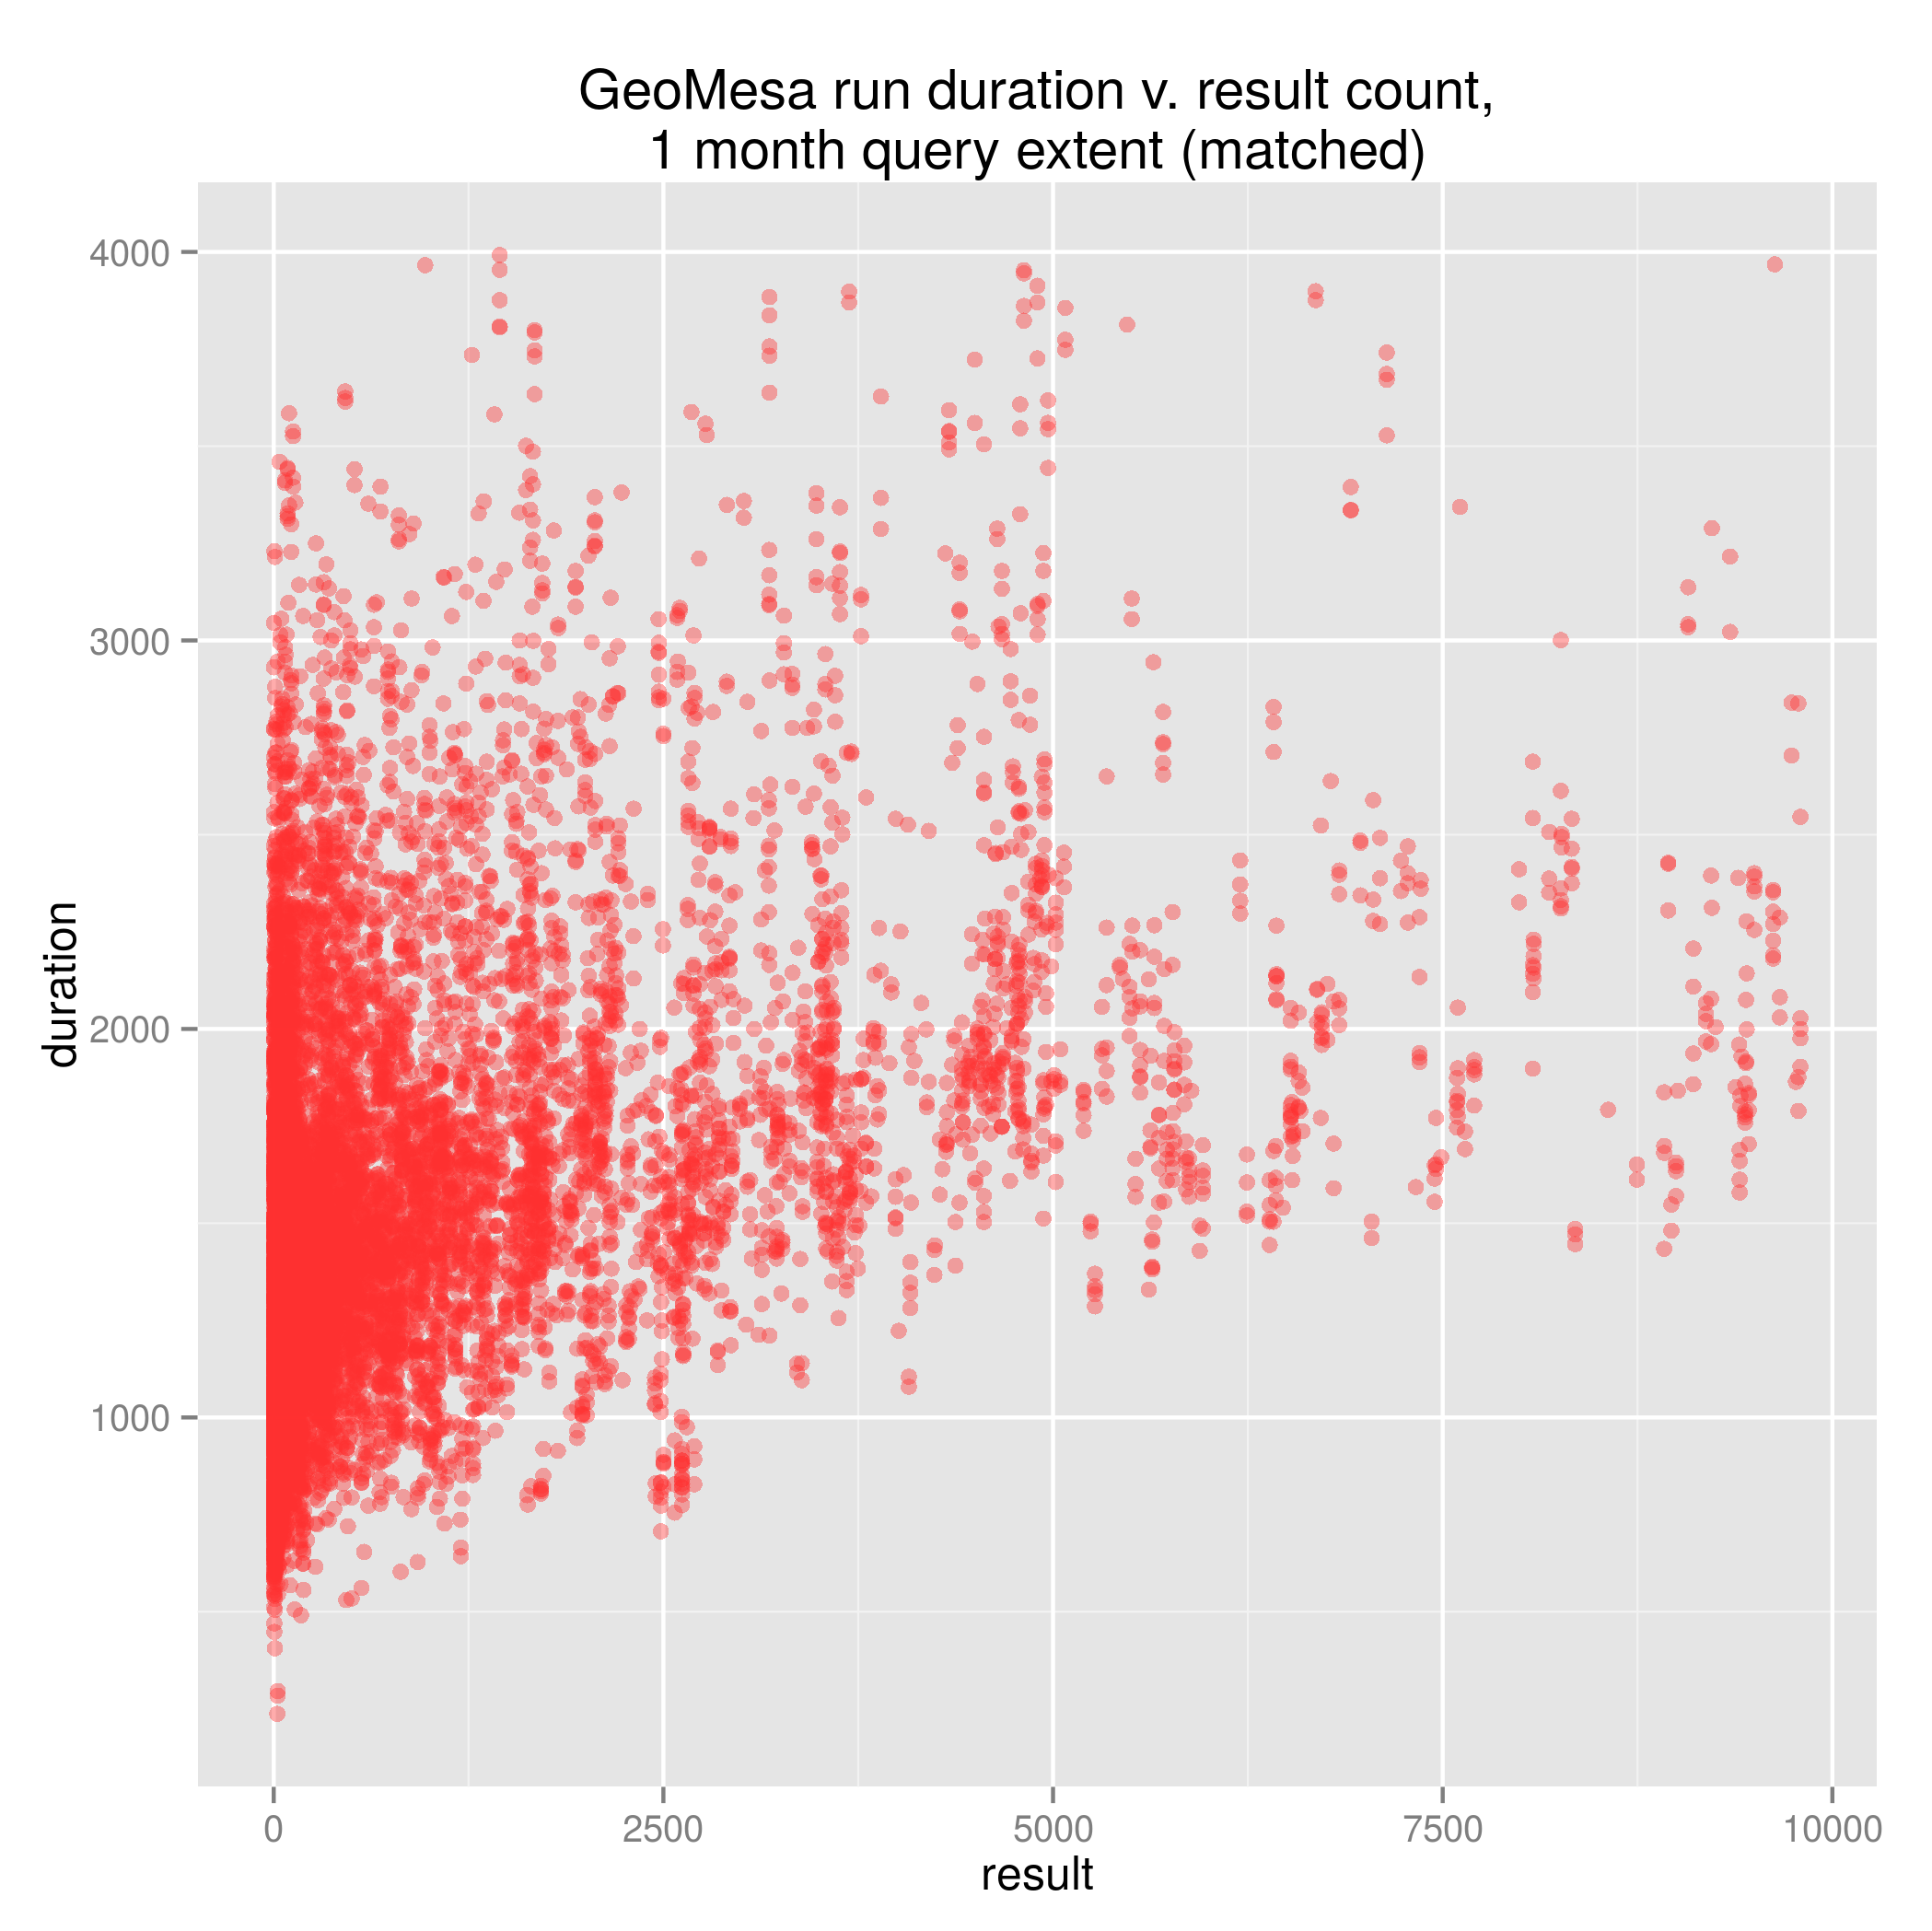
\includegraphics[width=0.60\textwidth]{../docs/img/tracks/GM_duration_v_result_matched_1month.png}
  \caption{GeoMesa duration versus results.}
  \label{tracksgm}
\end{figure}

\begin{figure}[h!tb]
  \centering
  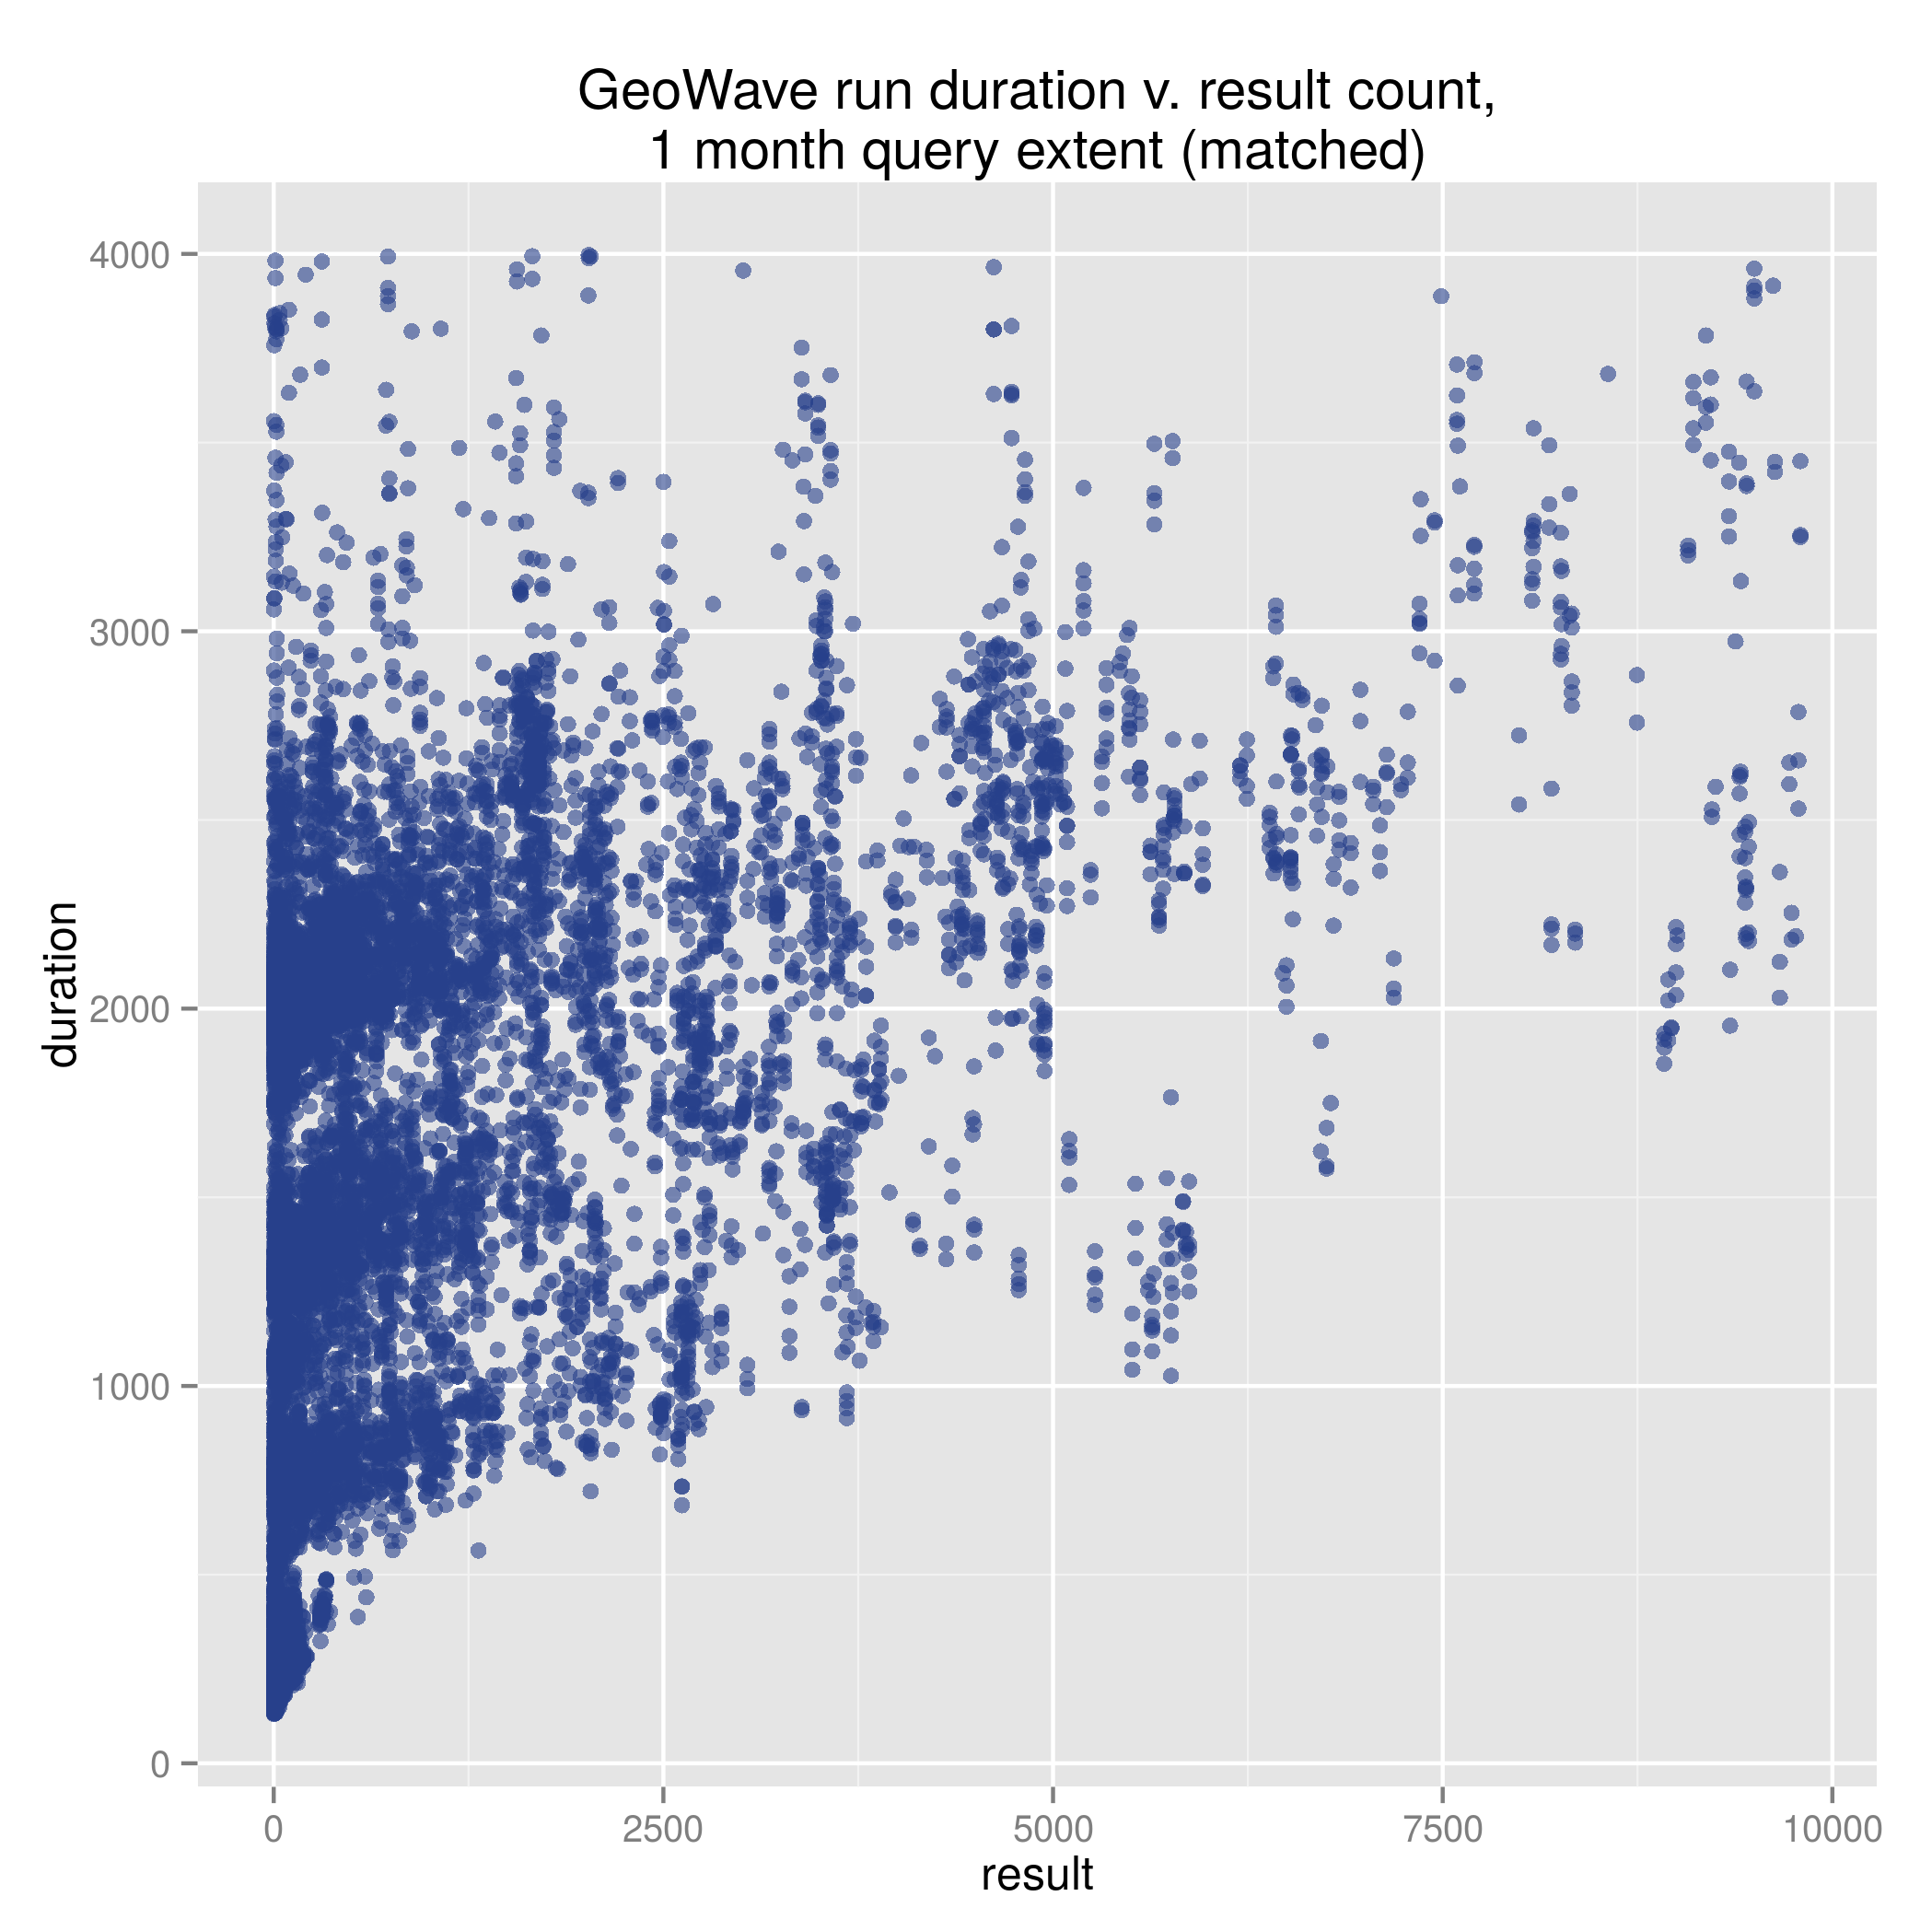
\includegraphics[width=0.60\textwidth]{../docs/img/tracks/GW_duration_v_result_matched_1month.png}
  \caption{GeoWave duration versus results.}
  \label{tracksgw}
\end{figure}

There is an indication of a gentle upward trend in both the case of GeoWave and GeoMesa;
however, the GeoWave results exhibit an additional tendency for the returns to stratify.
This behavior is possibly an artifact of GeoWave's tiering strategy and would only appear in datasets with elements that exhibit a range of geometric extents,
which is the case for this dataset.

Below is a chart that represents the distribution of durations for each system, as well as marking the mean duration.
It shows GeoMesa performing better on this dataset, which is consistent with our analysis.
Please see Figure \ref{tracksgmgw}.

\begin{figure}[h!tb]
  \centering
  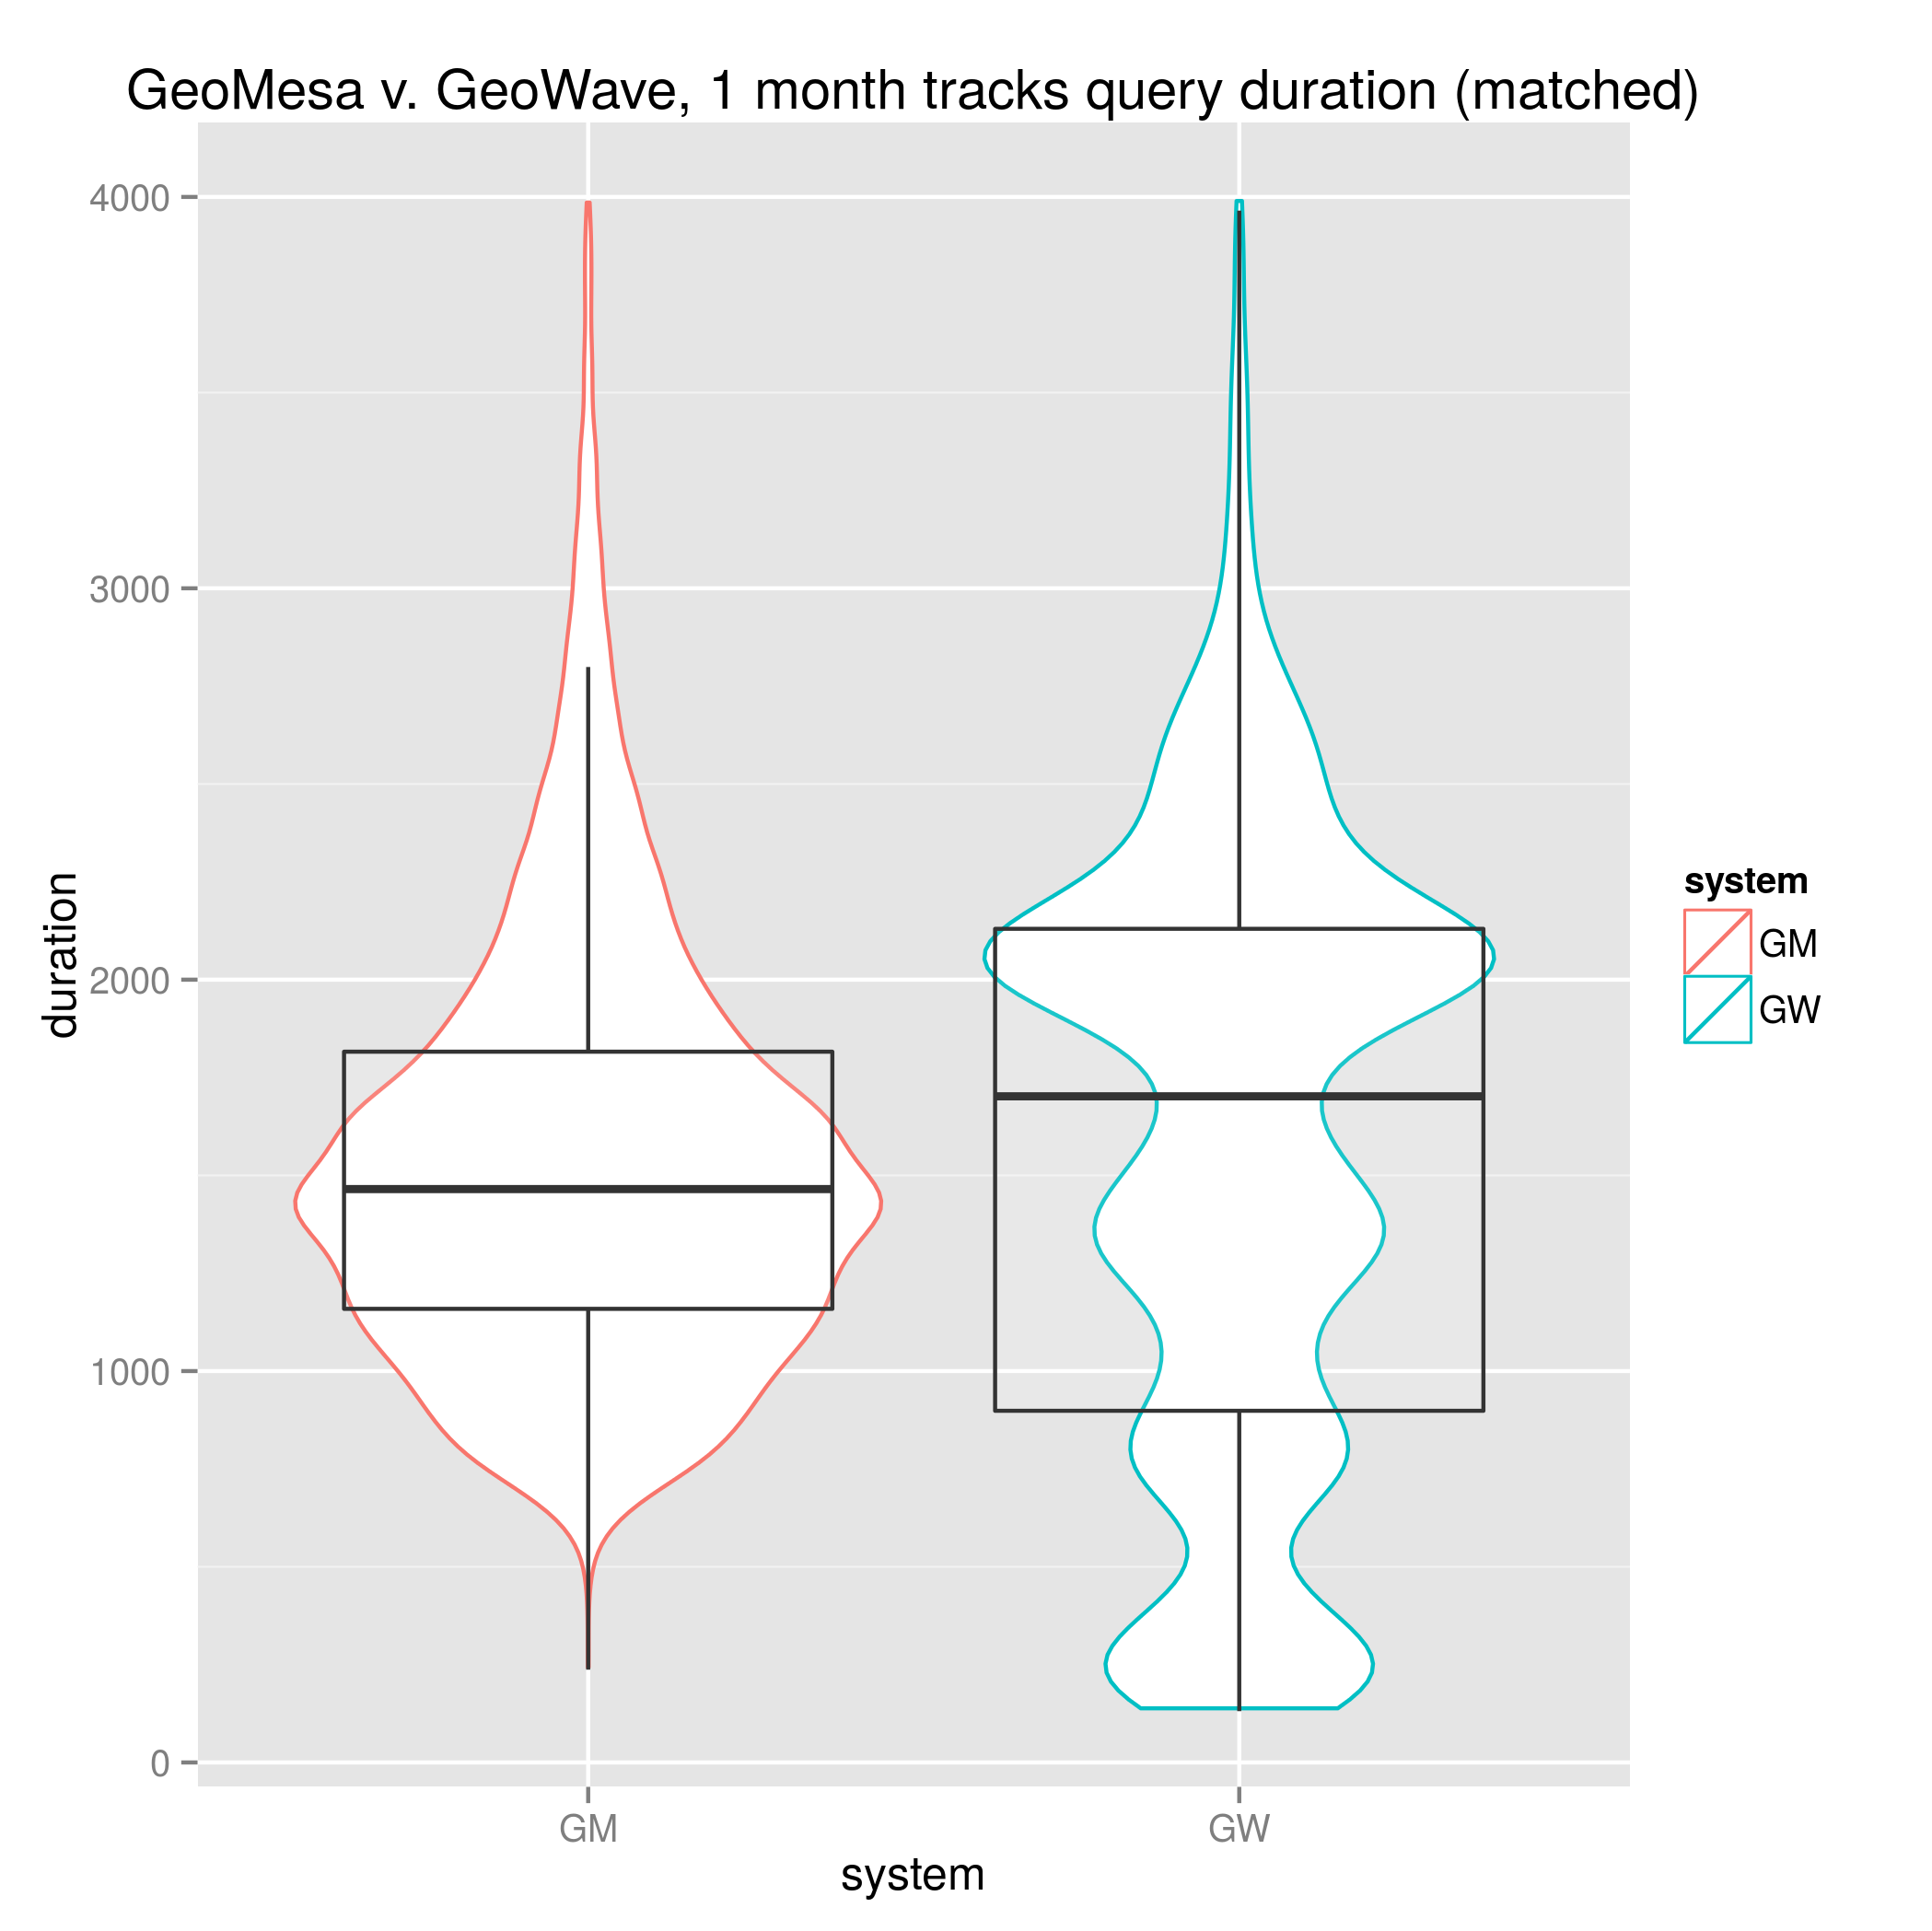
\includegraphics[width=0.60\textwidth]{../docs/img/tracks/GM_GW_tracks_duration_matched_1month.png}
  \caption{GeoMesa and GeoWave on the Tracks dataset.}
  \label{tracksgmgw}
\end{figure}

If we look at the mean durations over result count groupings according to a quantile-based discretization function of result count
(Figure \ref{tracksdurationresult}),
we see GeoMesa consistently outperforming GeoWave.

\begin{figure}[h!tb]
  \centering
  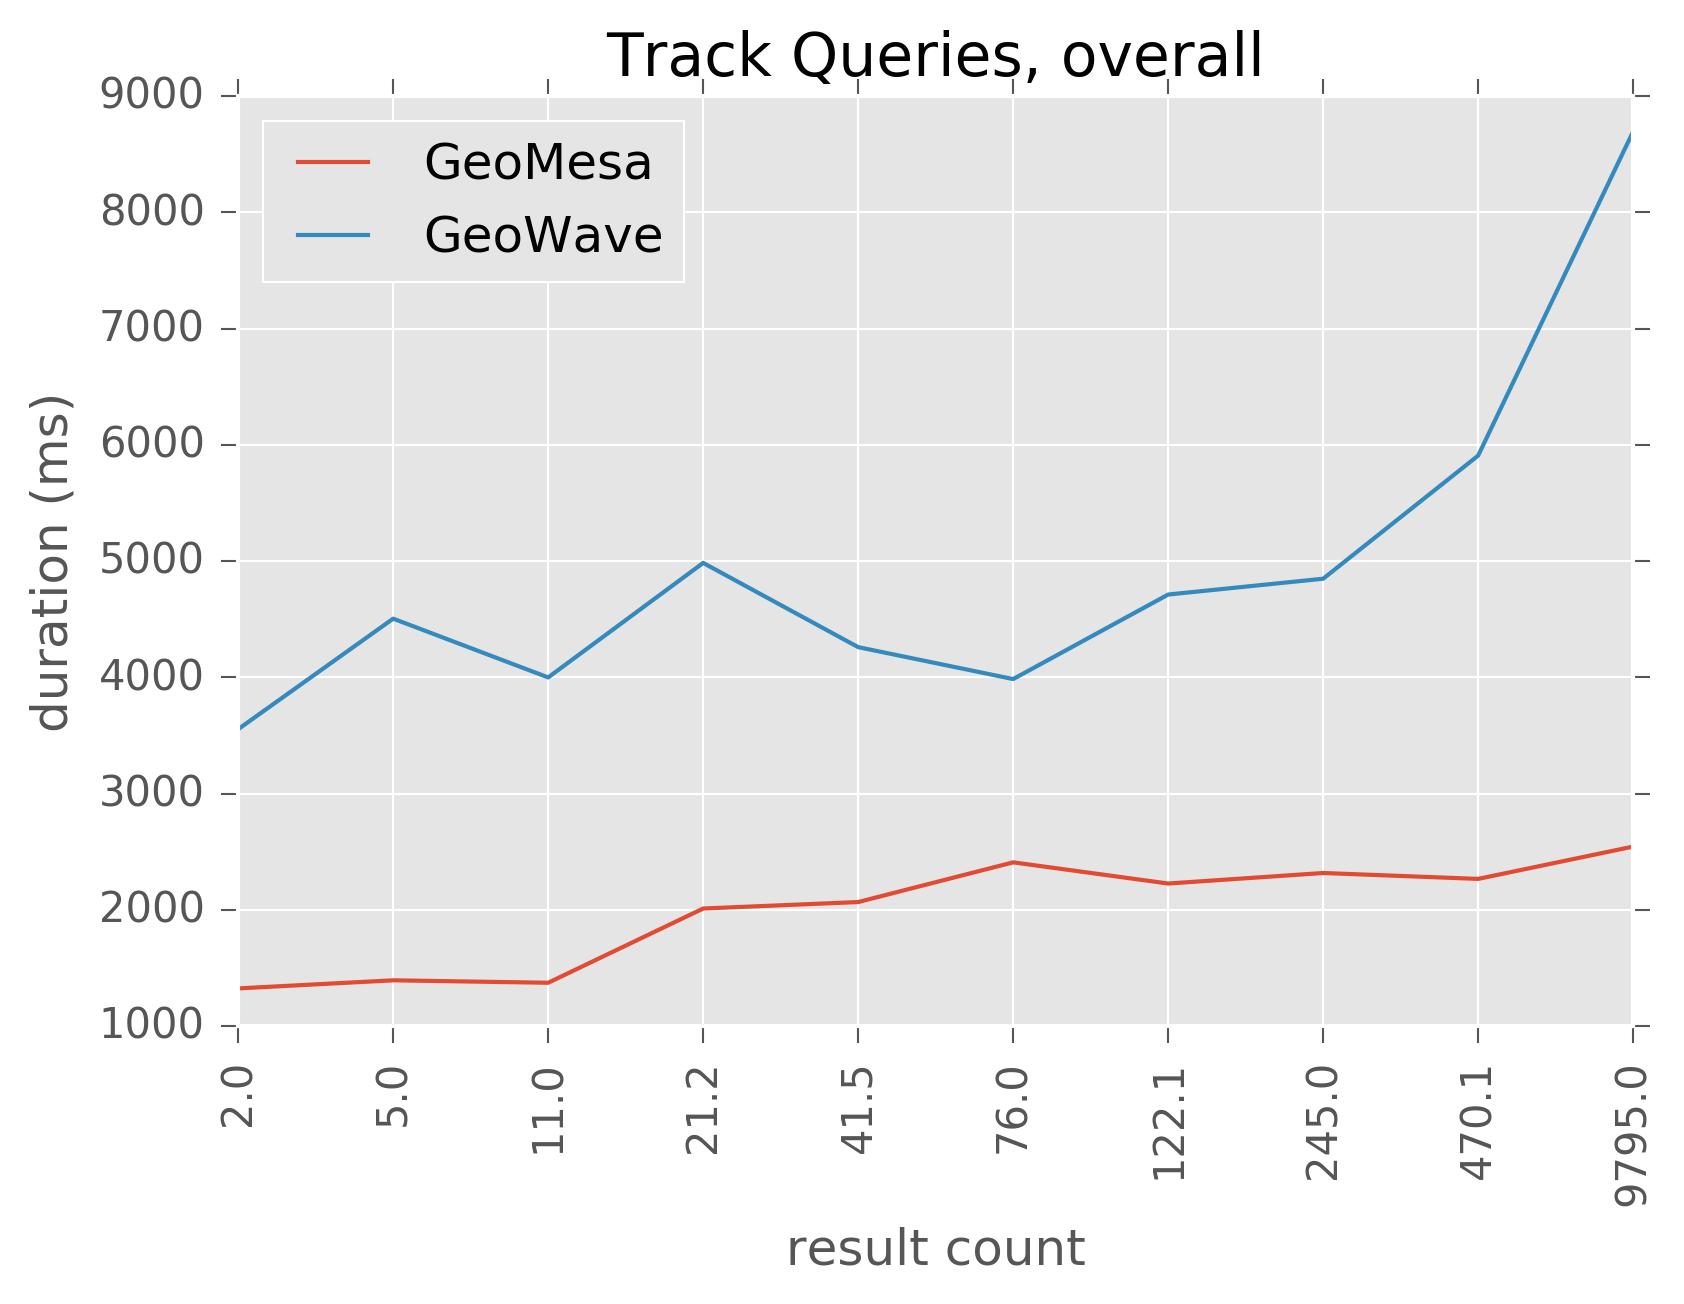
\includegraphics[width=0.60\textwidth]{../docs/img/tracks/duration-by-result-count.png}
  \caption{Durations by result, by level.}
  \label{tracksdurationresult}
\end{figure}

To understand if there is a relationship between the temporal bounds of the query and performance,
we can look at the above chart broken down by the $5$ day, $18$ day and $27$ day queries.
For GeoMesa, we do not see a clear behavior (Figure \ref{tracksgm2}).
But for GeoWave, the performance seems to be correlated with the size of the temporal query bounds (Figure \ref{tracksgw2}).

\begin{figure}[h!tb]
  \centering
  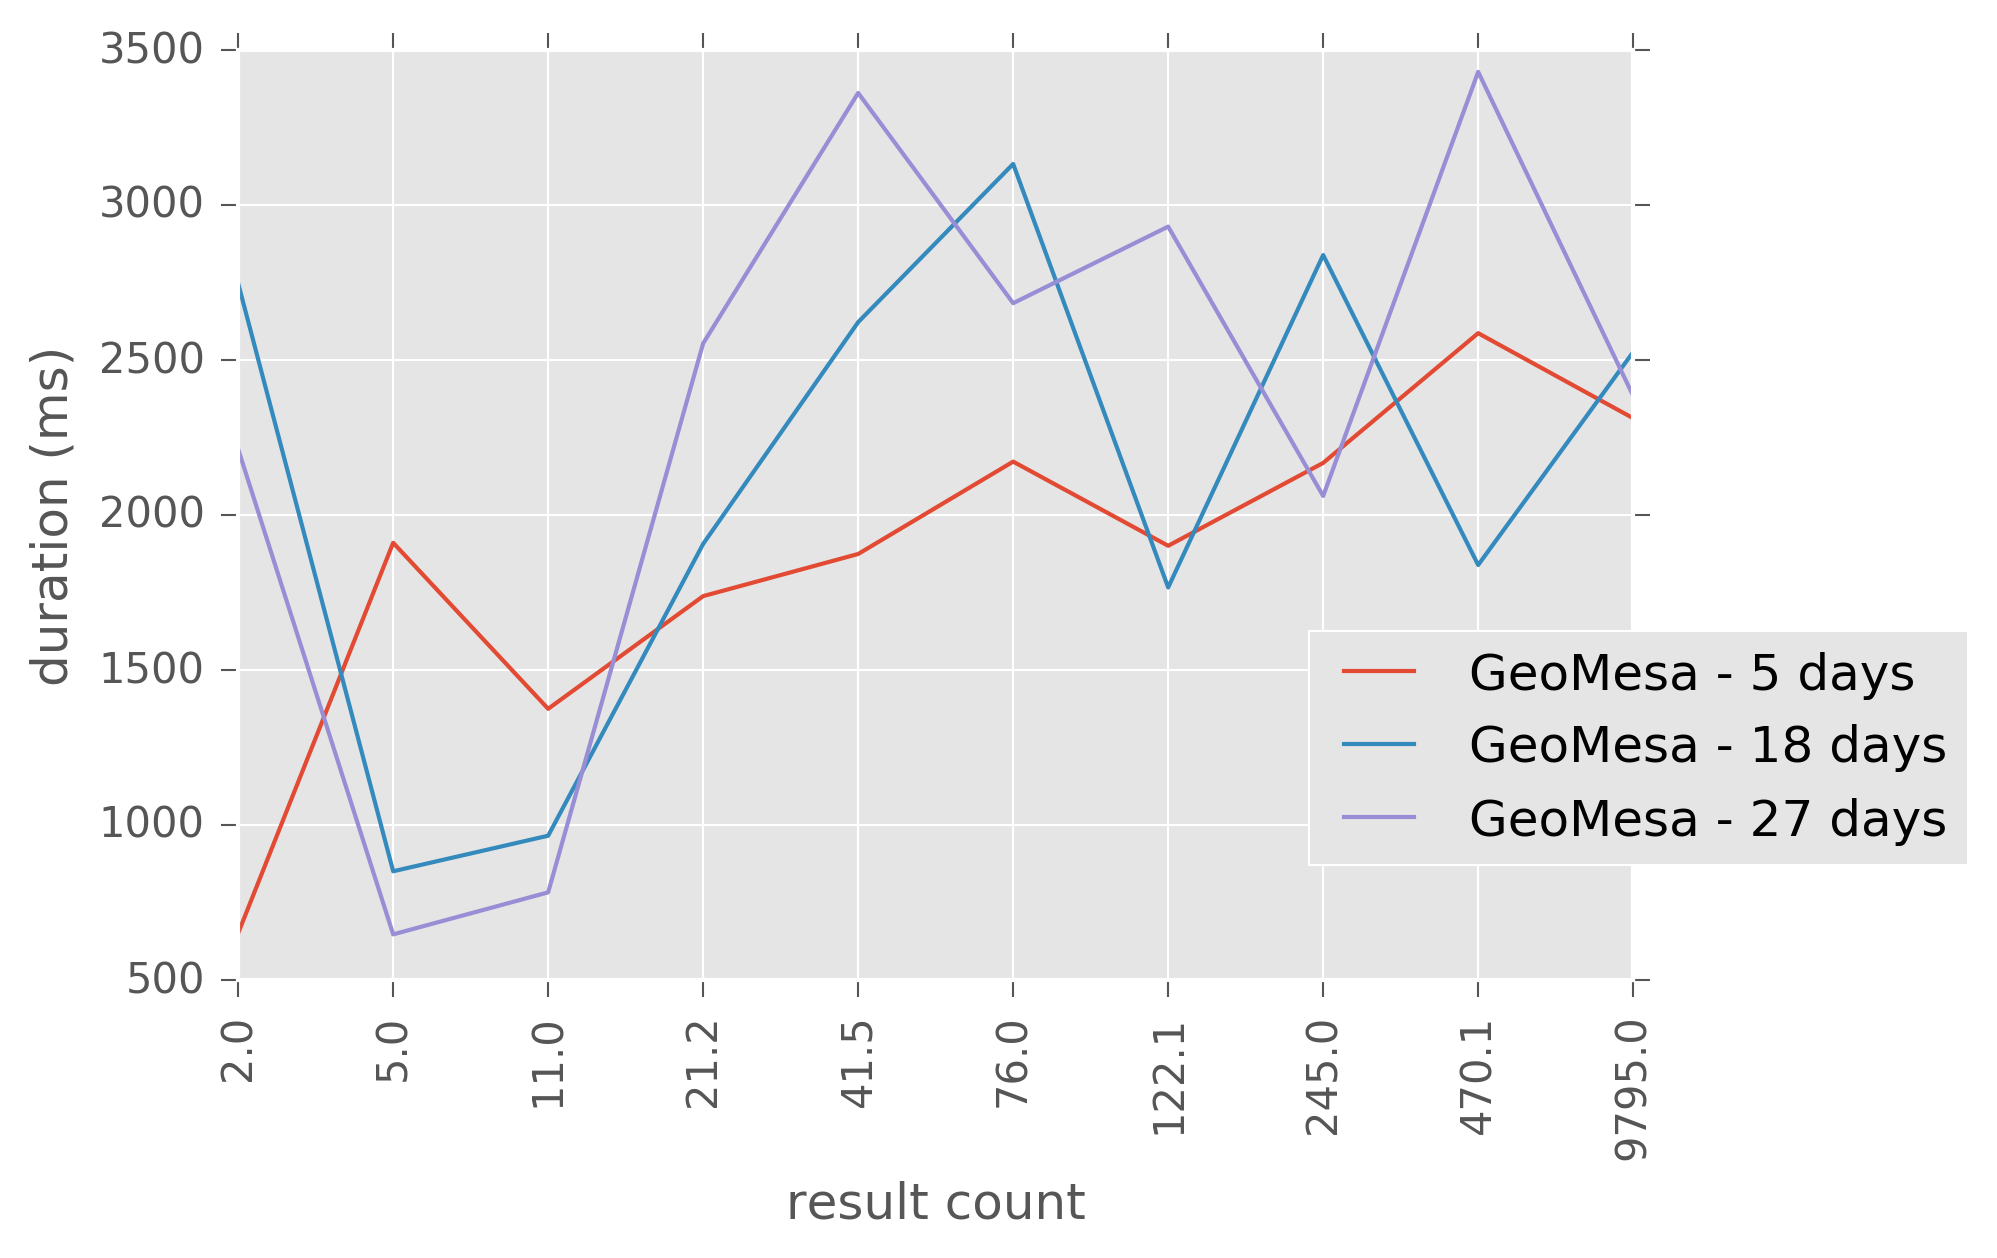
\includegraphics[width=0.60\textwidth]{../docs/img/tracks/geomesa-duration-by-result-count-and-days.png}
  \caption{Durations by result, by level for GeoMesa.}
  \label{tracksgm2}
\end{figure}

\begin{figure}[h!tb]
  \centering
  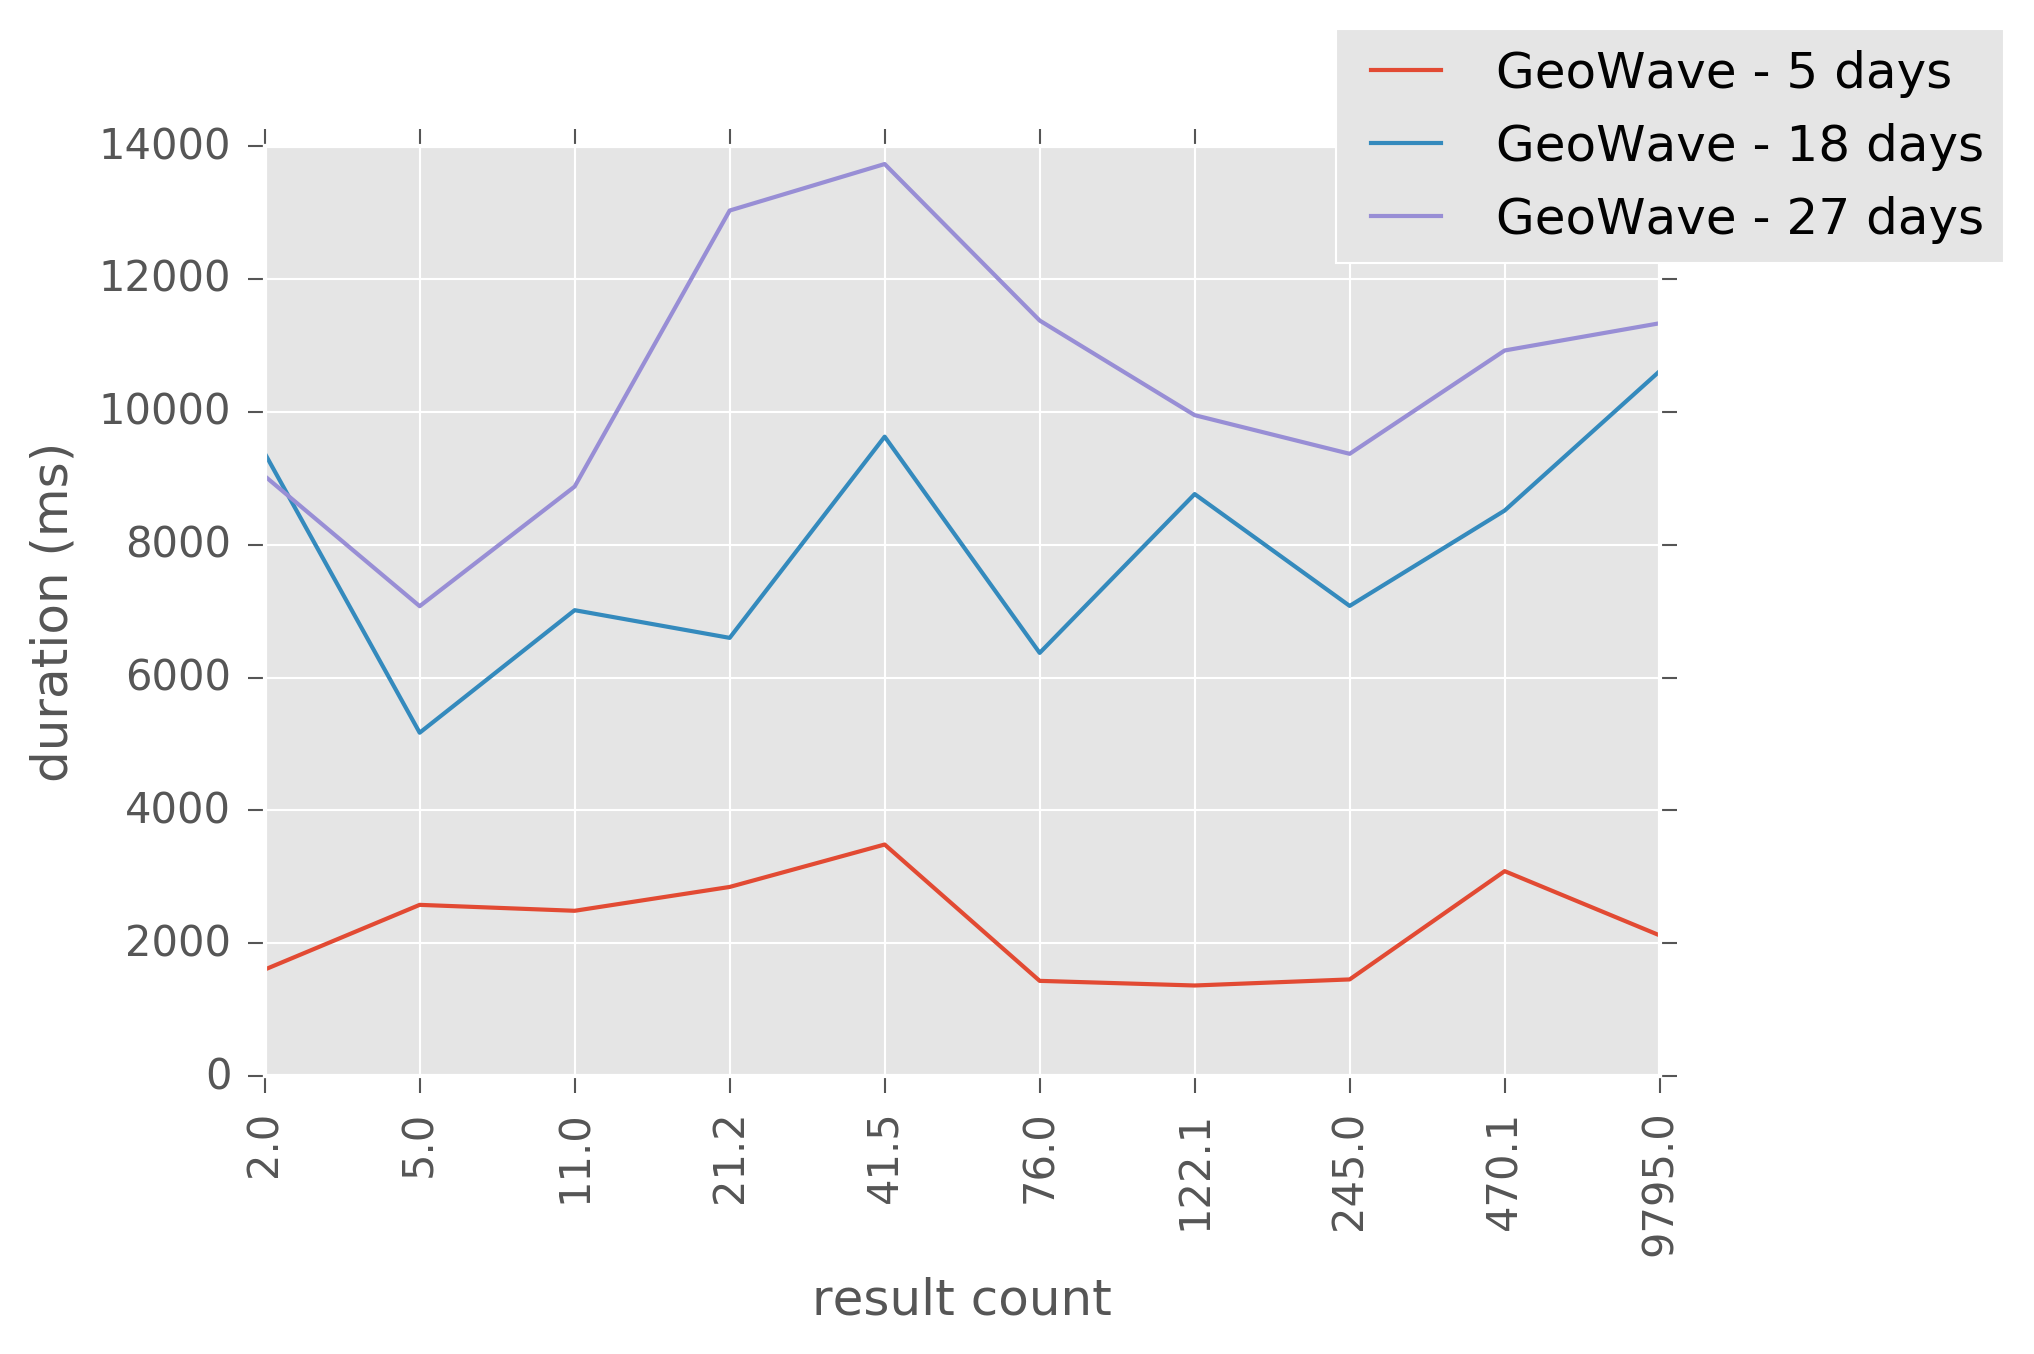
\includegraphics[width=0.60\textwidth]{../docs/img/tracks/geowave-duration-by-result-count-and-days.png}
  \caption{Durations by result, by level for GeoWave.}
  \label{tracksgw2}
\end{figure}
